\documentclass[12pt,a4paper]{article}

\usepackage[utf8]{inputenc}
\usepackage[T1]{fontenc}
\usepackage[polish]{babel}
\usepackage{graphicx}
\usepackage{float}
\usepackage{booktabs}
\usepackage{geometry}
\usepackage{amsmath}
\usepackage{hyperref}
\usepackage{caption}
\usepackage{subcaption}
\usepackage{array}
\usepackage{xcolor}

\geometry{margin=2.5cm}

\title{Lista 2: Wyżarzanie i Tabu Search Alogrytmy metaheurystyczne}
\author{Jakub Kogut}
\date{\today}

\begin{document}

\maketitle

\section{Cel ćwiczenia}

Celem ćwiczenia było zaimplementowanie oraz eksperymentalne przetestowanie dwóch metaheurystyk służących do rozwiązywania problemu komiwojażera: symulowanego wyżarzania oraz algorytmu Tabu Search. Następnie przeprowadzono eksperymenty na instancjach TSP o różnej liczbie wierzchołków:

\begin{itemize}
    \item \texttt{eg7146.tsp},
    \item \texttt{ar9152.tsp},
    \item \texttt{it16862.tsp}.
\end{itemize}

\section{Symulowane wyżarzanie}

\subsection{Opis metody}

Symulowane wyżarzanie jest metaheurystyką inspirowaną procesem chłodzenia metalu. Algorytm rozpoczyna działanie od losowego rozwiązania, a następnie iteracyjnie generuje rozwiązania sąsiednie.

Jeżeli nowe rozwiązanie jest lepsze, zostaje zaakceptowane zawsze. Jeżeli jest gorsze, może zostać zaakceptowane z pewnym prawdopodobieństwem zależnym od temperatury oraz pogorszenia jakości rozwiązania. W implementacji minimalizowano długość trasy, dlatego dla pogorszenia $\Delta > 0$ prawdopodobieństwo akceptacji wynosiło:

\[
p = e^{-\Delta/T}.
\]

Wraz ze spadkiem temperatury algorytm coraz rzadziej akceptował gorsze rozwiązania, przez co przechodził od fazy eksploracji do fazy eksploatacji.

\subsection{Zastosowane parametry}

W programie można było zmieniać następujące parametry:

\begin{itemize}
    \item \texttt{--temp} -- temperatura początkowa,
    \item \texttt{--cooling} -- współczynnik chłodzenia,
    \item \texttt{--trials} -- liczba prób w jednej epoce,
    \item \texttt{--epochs} -- maksymalna liczba epok,
    \item \texttt{--no-improve} -- limit epok bez poprawy,
\end{itemize}

Wybór parametrów przeprowadzano eksperymentalnie. Dla temperatury początkowej oraz współczynnika chłodzenia przygotowano wykres typu heatmap, na którym oś X odpowiadała wartości \texttt{cooling}, oś Y temperaturze początkowej, a kolor oznaczał uzyskany koszt trasy.

\subsection{Dobór parametrów}

Dla małych i średnich instancji sprawdzono różne wartości temperatury początkowej oraz współczynnika chłodzenia. Zbyt niska temperatura powodowała szybkie zatrzymanie algorytmu w minimum lokalnym, ponieważ gorsze rozwiązania były rzadko akceptowane. Zbyt wysoka temperatura powodowała natomiast długie chaotyczne przeszukiwanie przestrzeni rozwiązań.

Współczynnik chłodzenia bliski $1$, np. $0.99$ lub $0.995$, powodował wolniejszy spadek temperatury, co zwykle poprawiało jakość rozwiązania kosztem dłuższego czasu działania. W praktyce najlepsze wyniki uzyskiwano dla większej liczby prób w epoce oraz powolnego chłodzenia.

\subsection{Wykresy dla symulowanego wyżarzania}

\subsubsection{Instancja \texttt{eg7146.tsp}}

\begin{figure}[H]
    \centering
    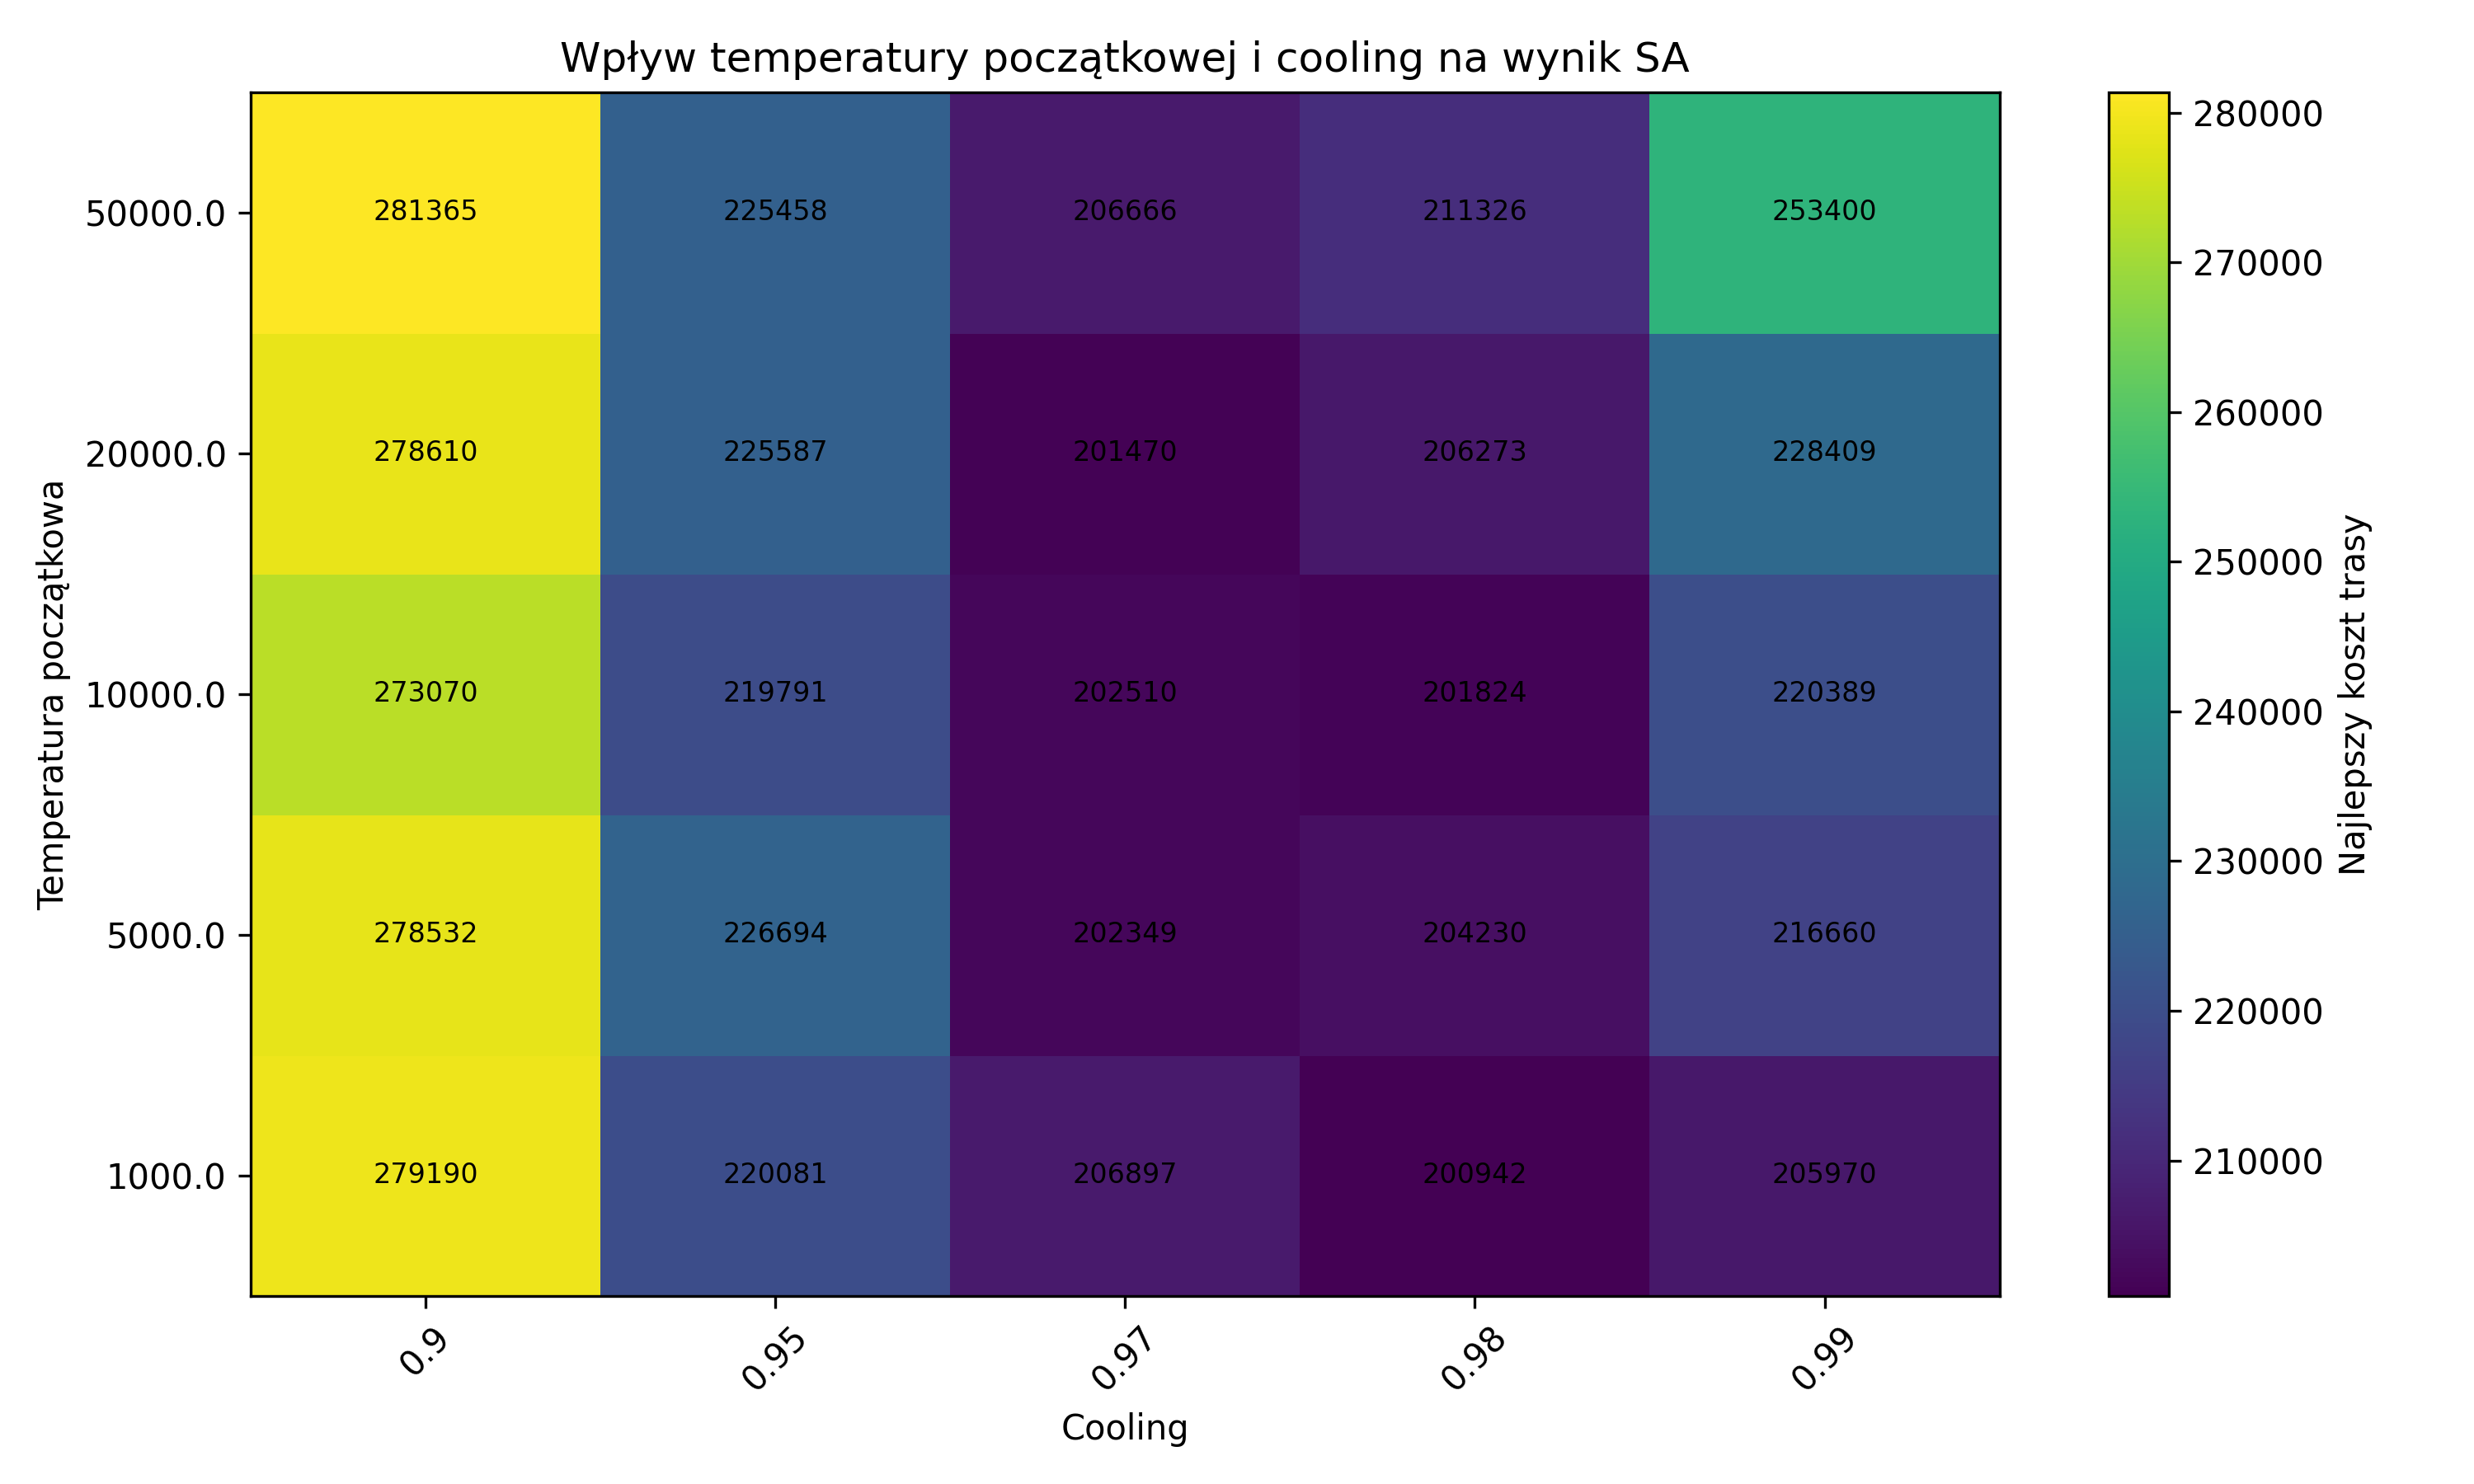
\includegraphics[width=0.9\textwidth]{temperature_grid_heatmap_eg7146.png}
    \caption{Wpływ temperatury początkowej i współczynnika chłodzenia na wynik algorytmu symulowanego wyżarzania dla instancji \texttt{eg7146.tsp}.}
\end{figure}

\begin{figure}[H]
    \centering
    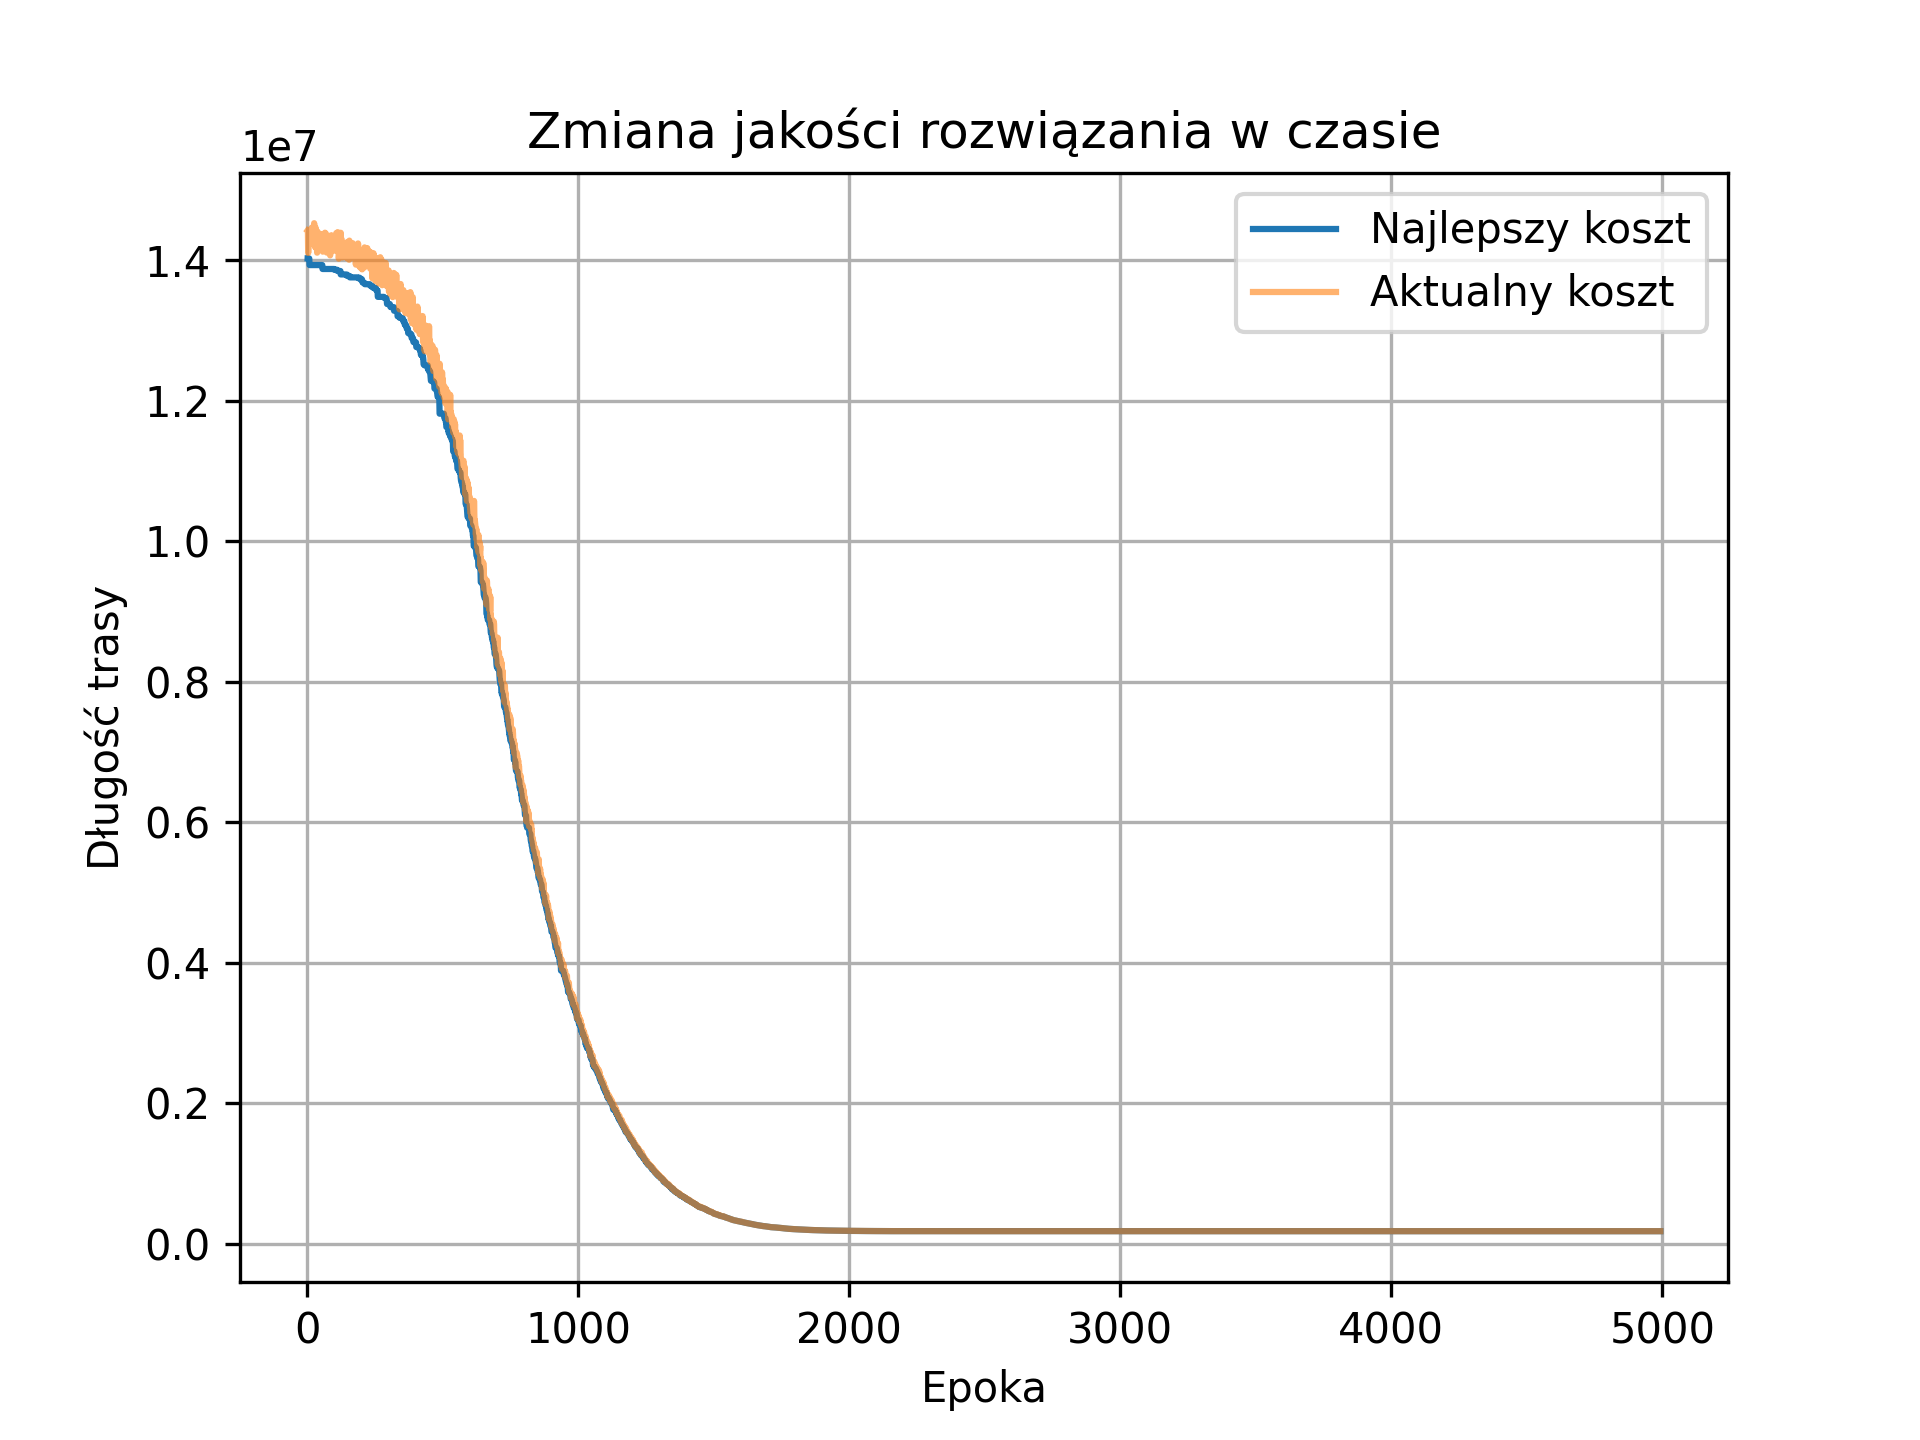
\includegraphics[width=0.9\textwidth]{cost_history_eg7146.png}
    \caption{Zmiana najlepszego i aktualnego kosztu w czasie dla instancji \texttt{eg7146.tsp}.}
\end{figure}

\begin{figure}[H]
    \centering
    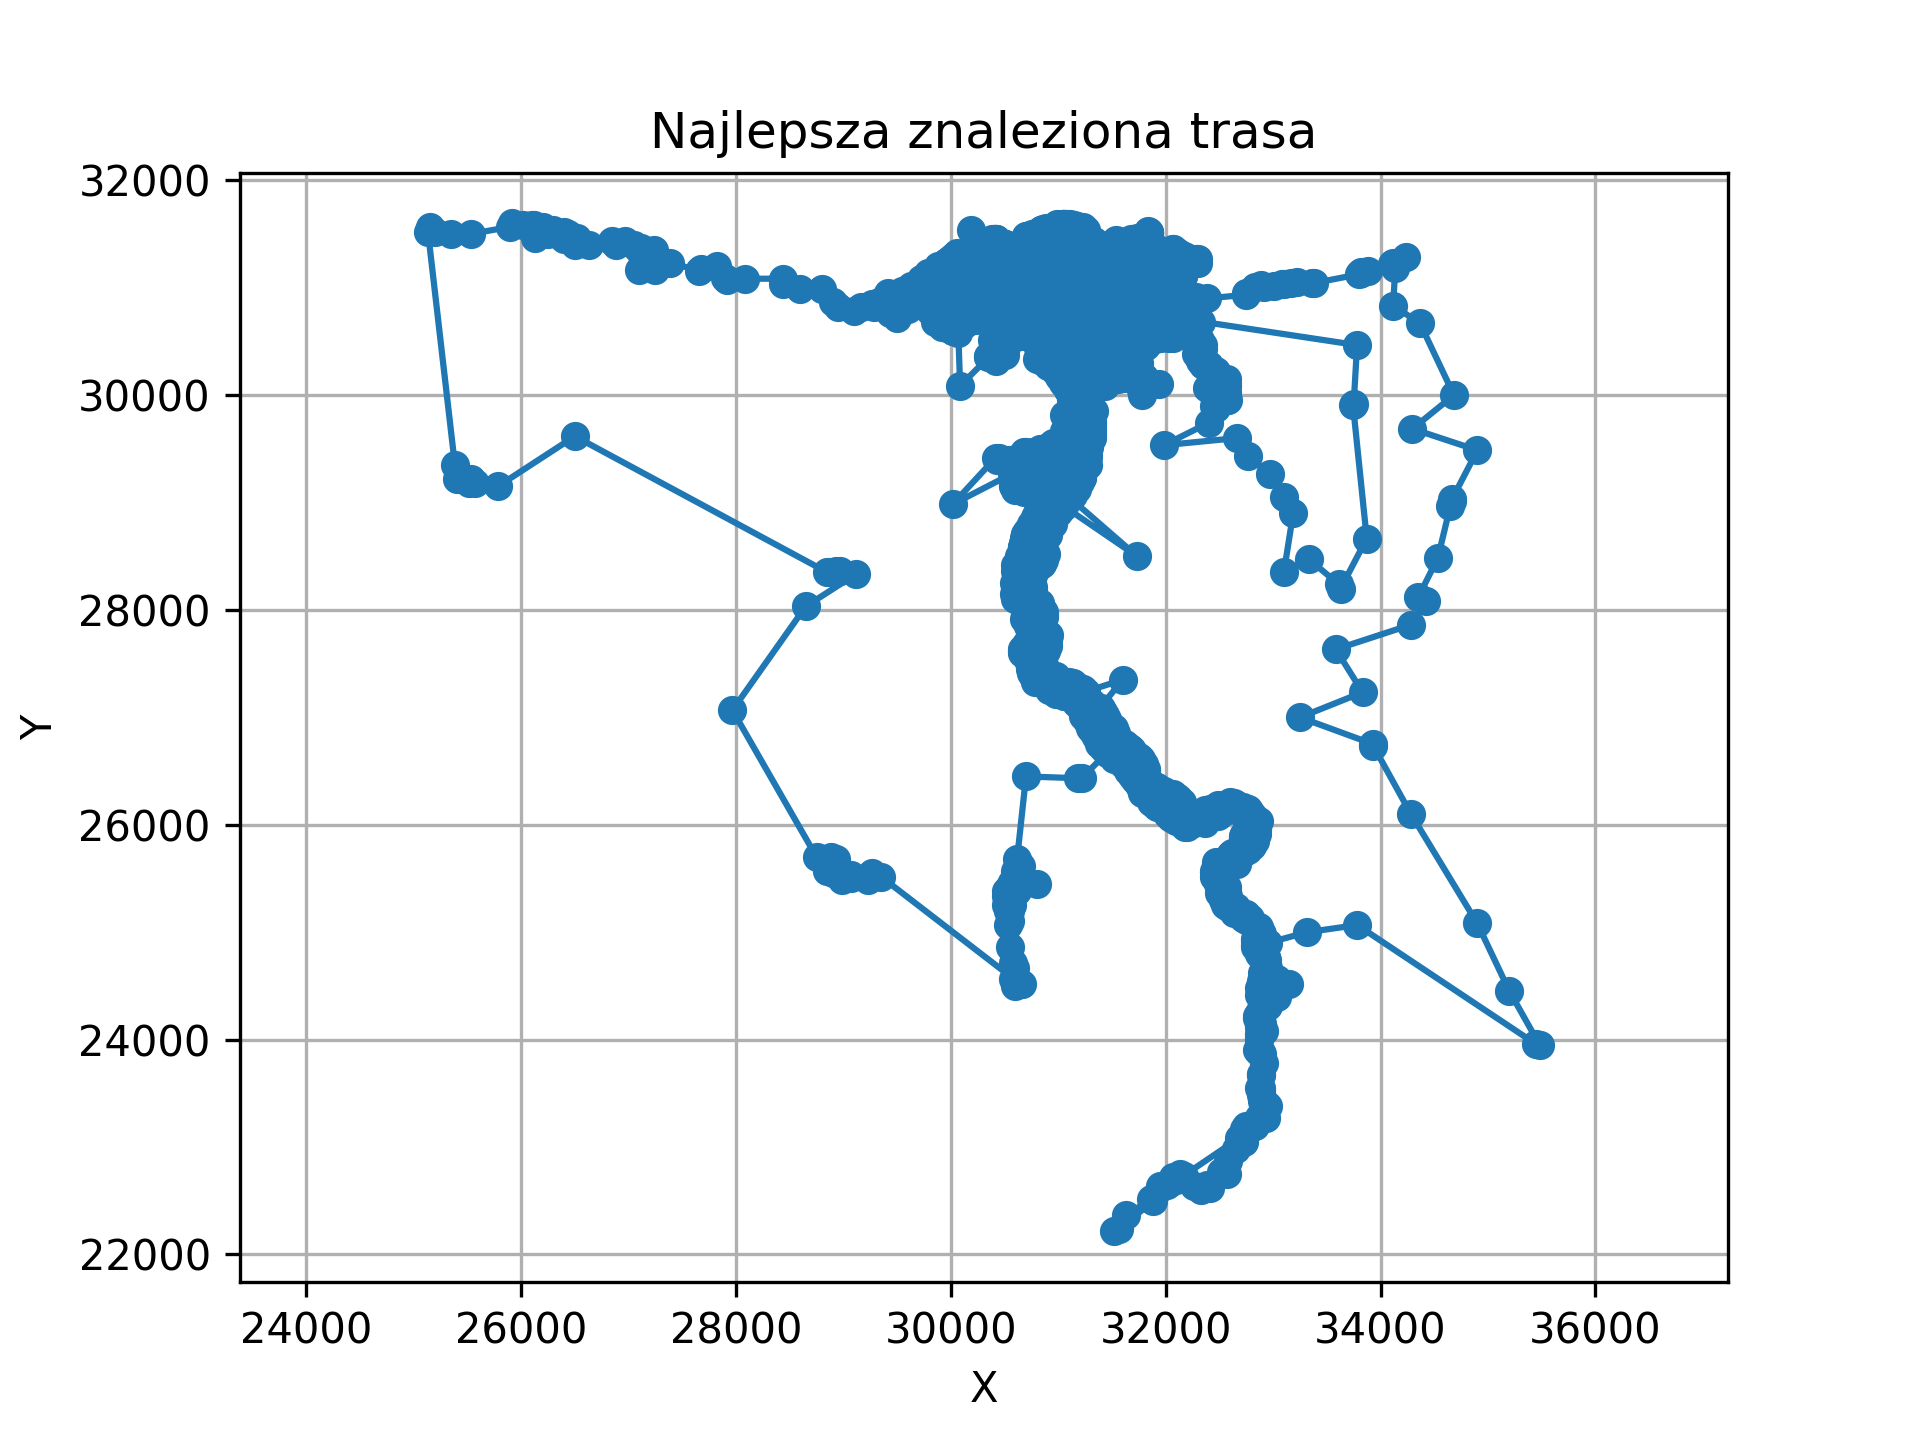
\includegraphics[width=0.8\textwidth]{best_route_eg7146.png}
    \caption{Najlepsza trasa znaleziona przez symulowane wyżarzanie dla instancji \texttt{eg7146.tsp}.}
\end{figure}

\subsubsection{Instancja \texttt{ar9152.tsp}}

\begin{figure}[H]
    \centering
    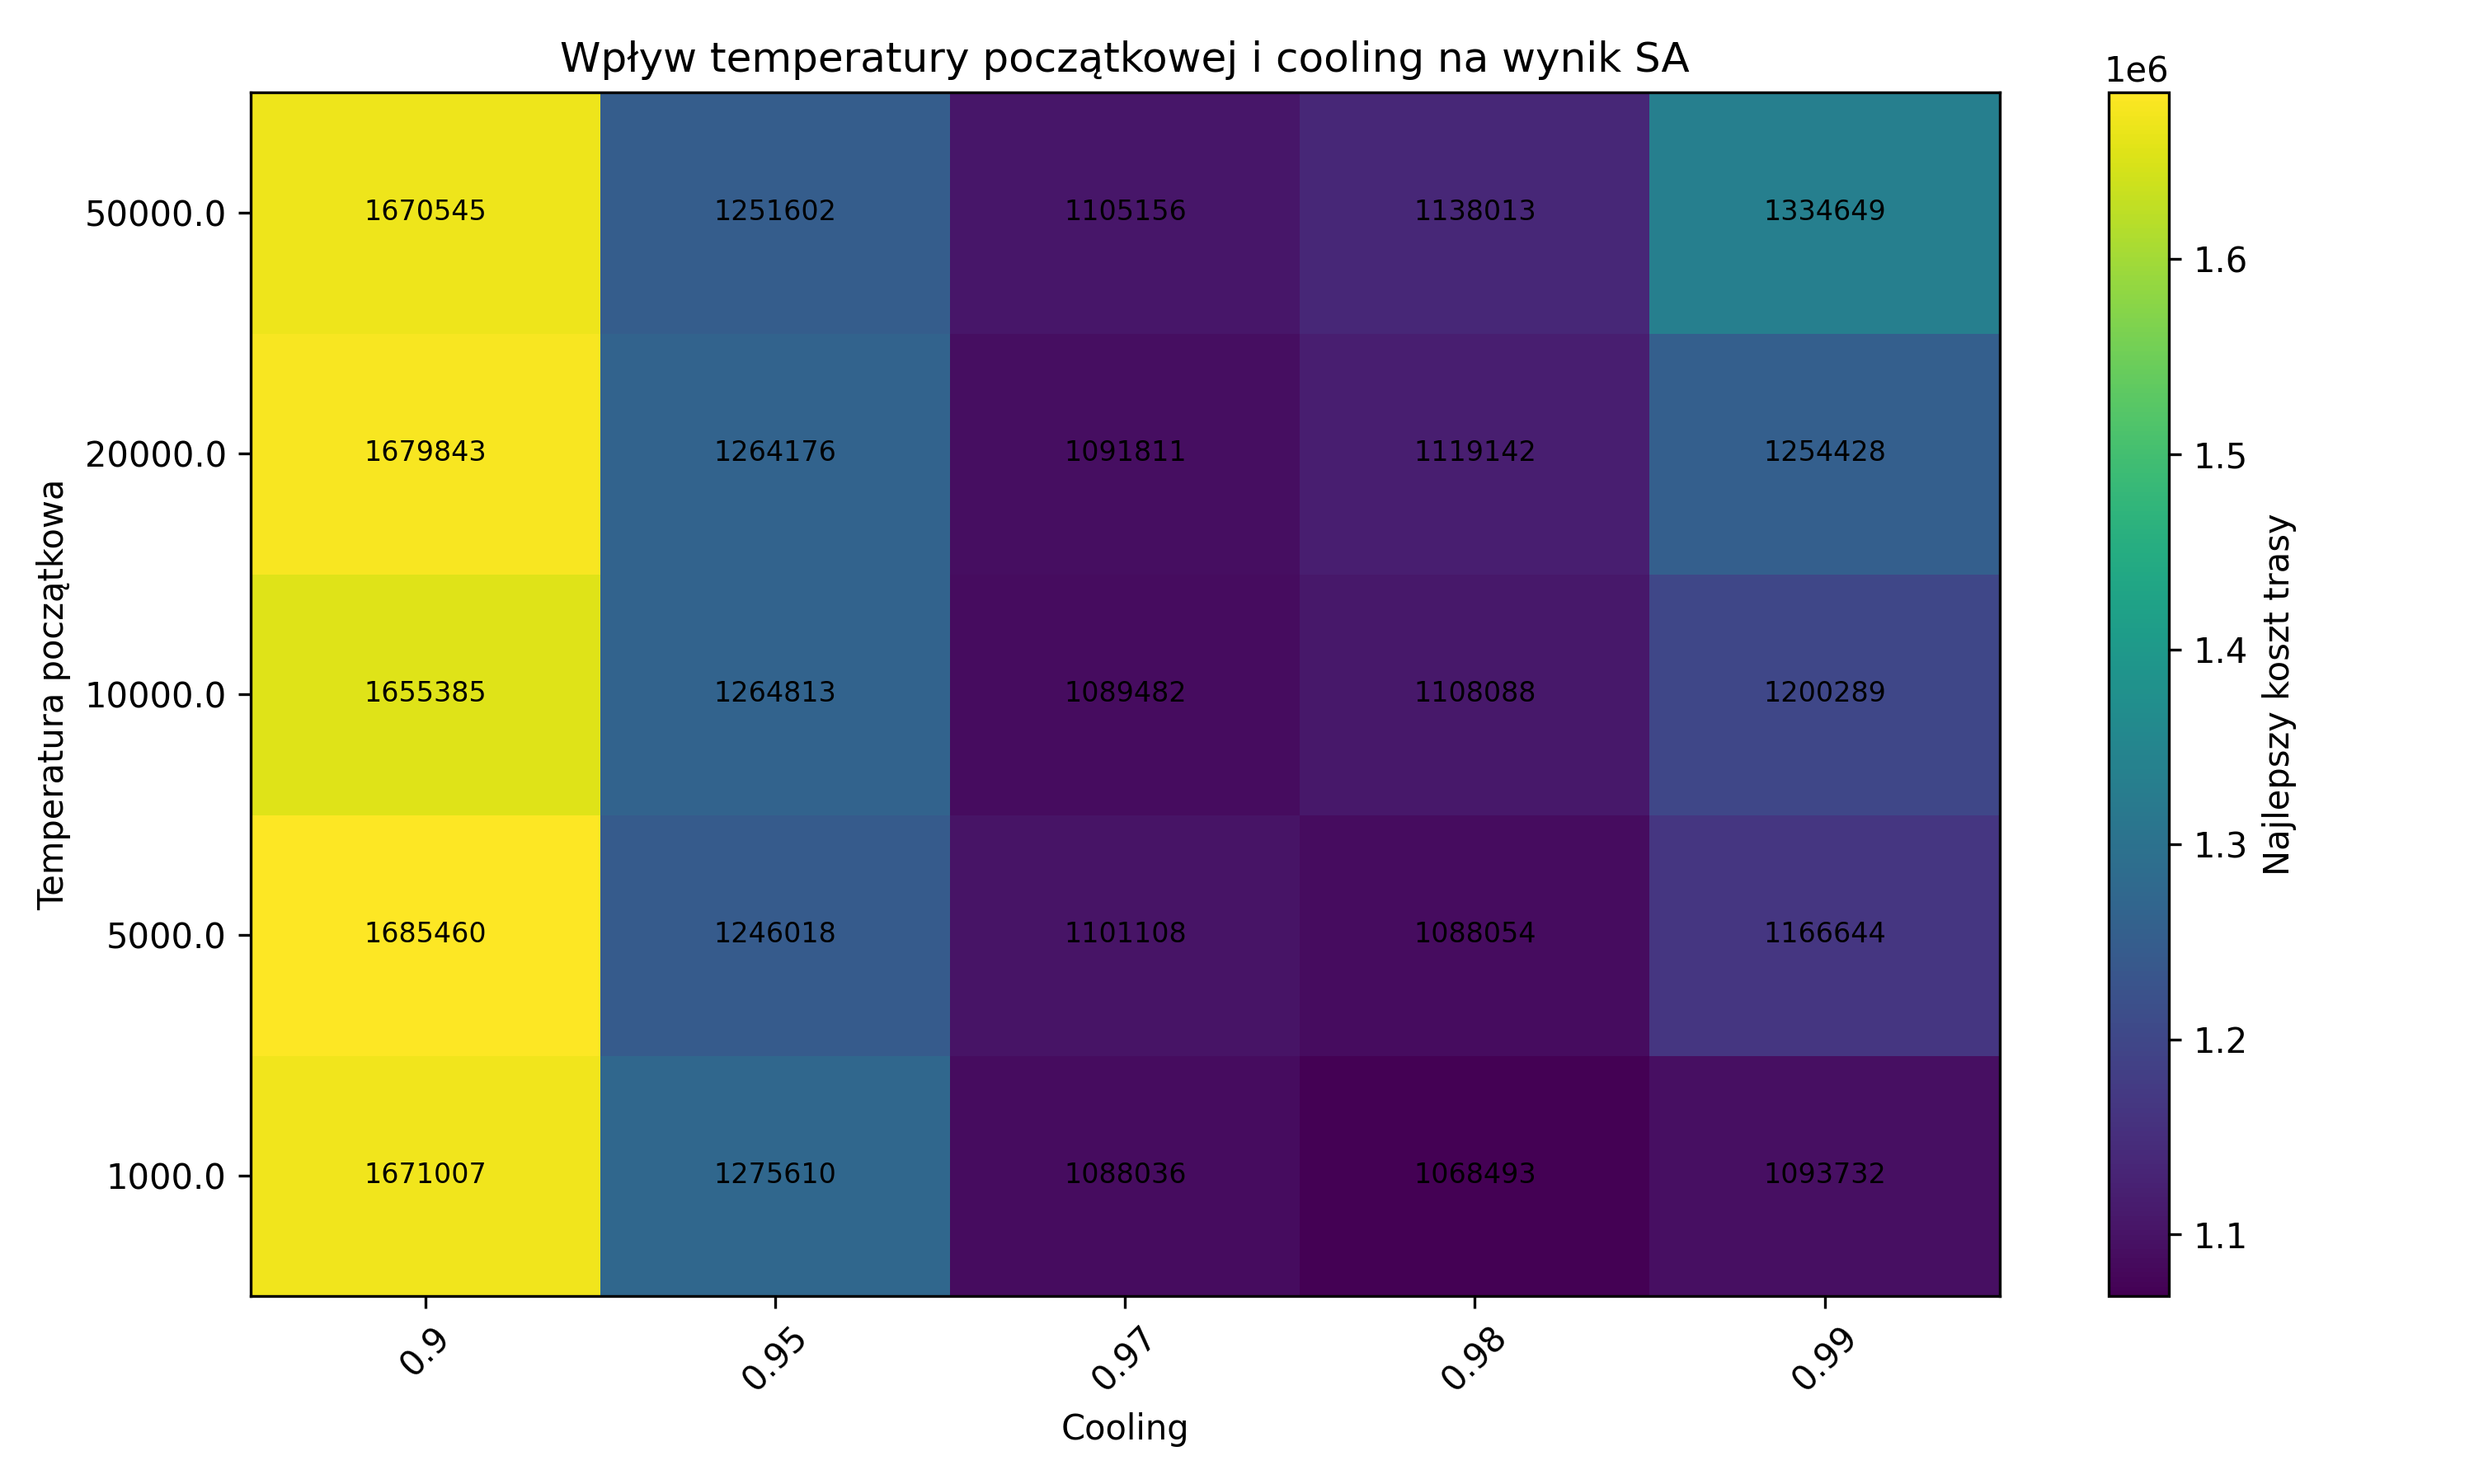
\includegraphics[width=0.9\textwidth]{temperature_grid_heatmap_ar9152.png}
    \caption{Wpływ temperatury początkowej i współczynnika chłodzenia na wynik algorytmu symulowanego wyżarzania dla instancji \texttt{ar9152.tsp}.}
\end{figure}

\begin{figure}[H]
    \centering
    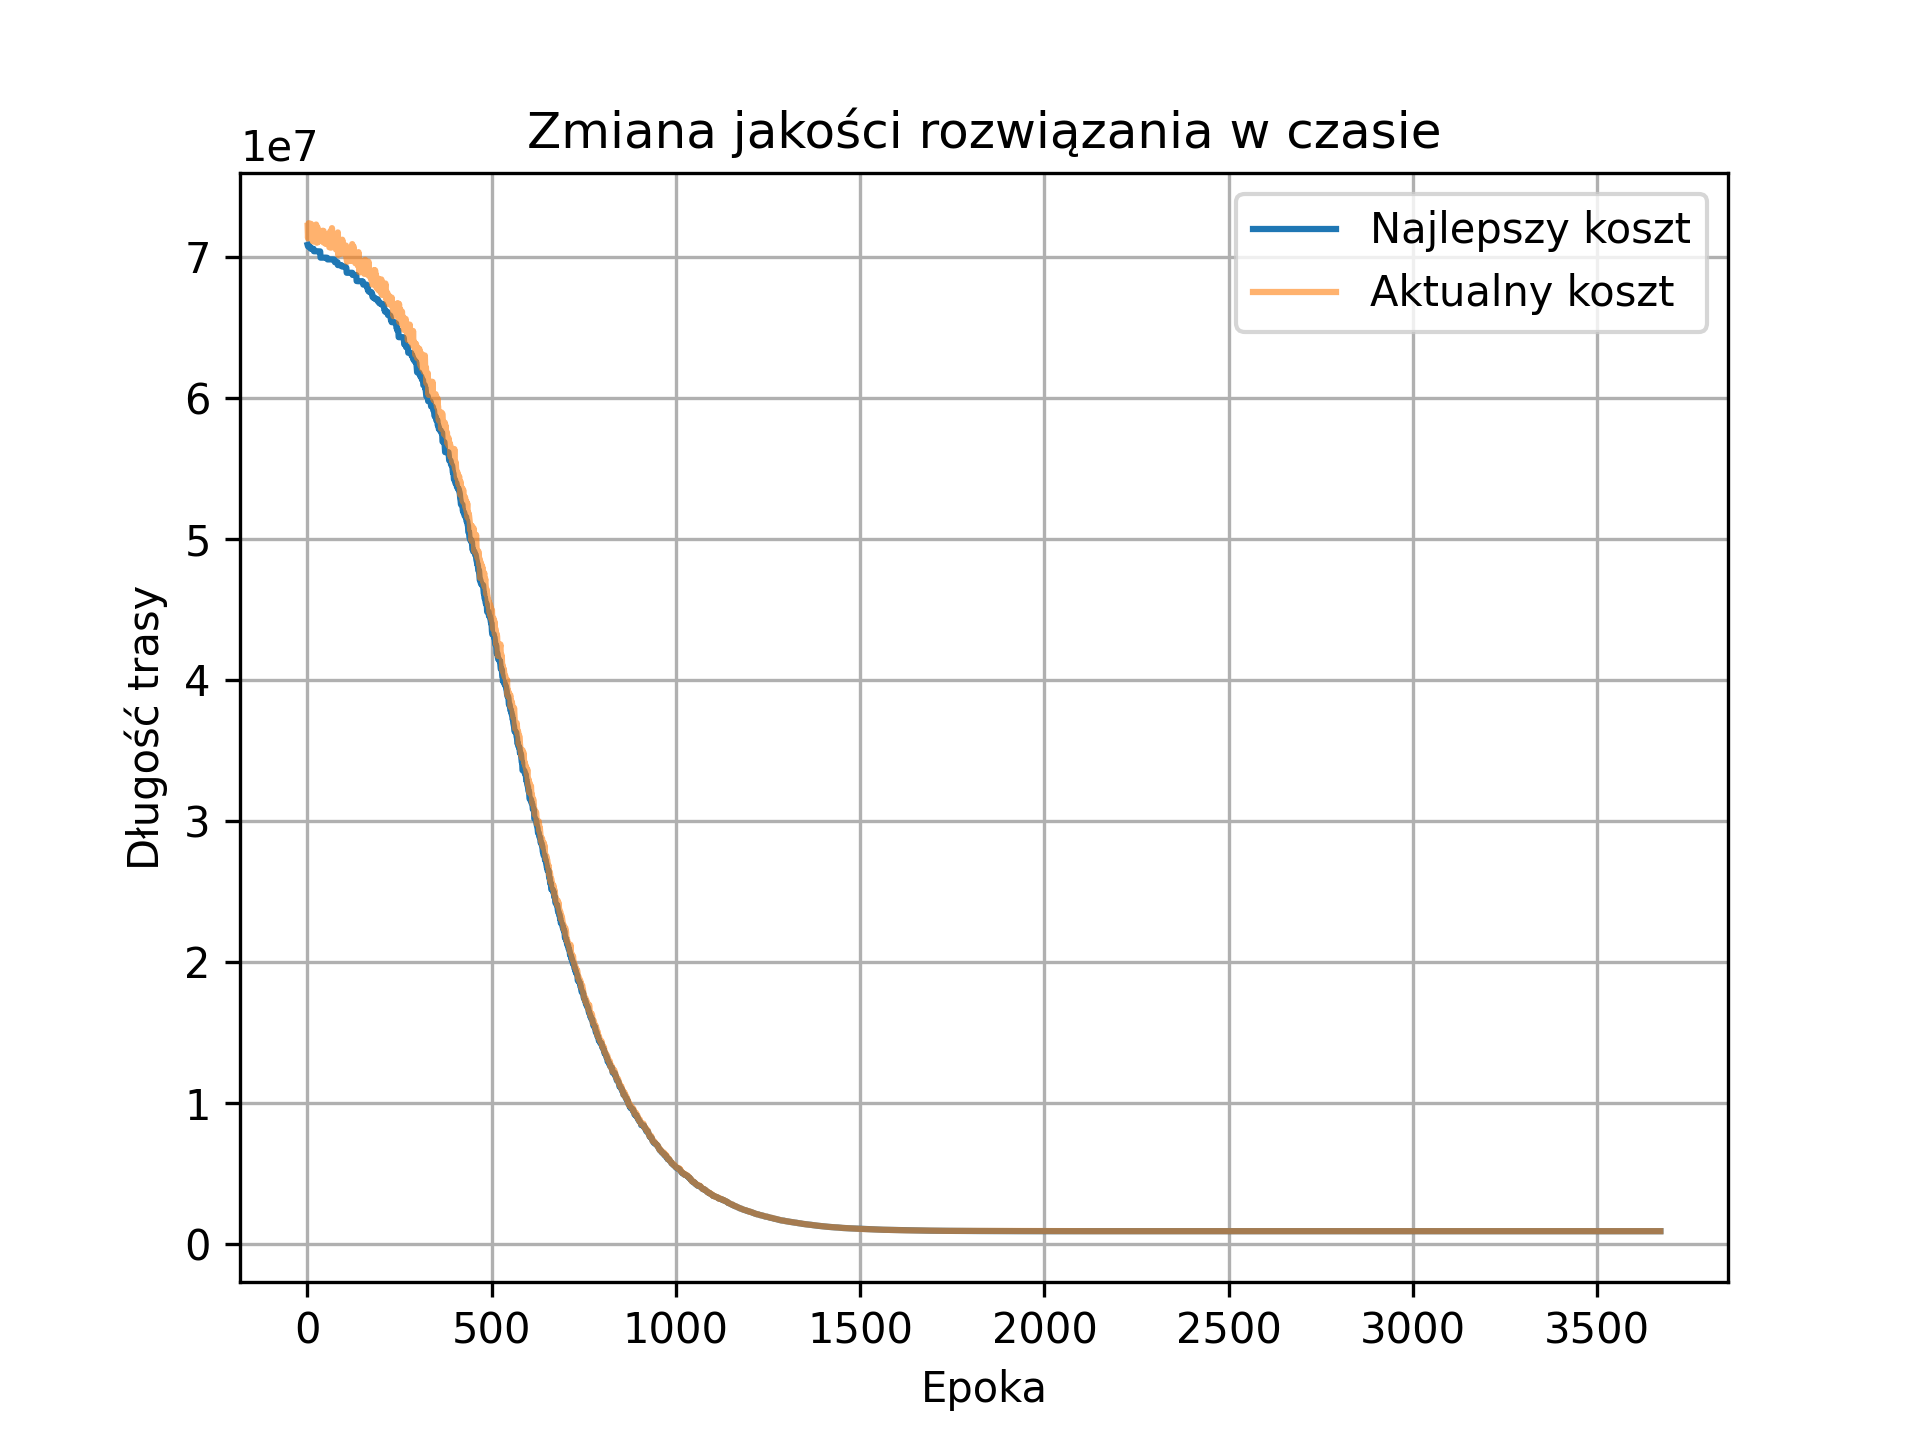
\includegraphics[width=0.9\textwidth]{cost_history_ar9152.png}
    \caption{Zmiana najlepszego i aktualnego kosztu w czasie dla instancji \texttt{ar9152.tsp}.}
\end{figure}

\begin{figure}[H]
    \centering
    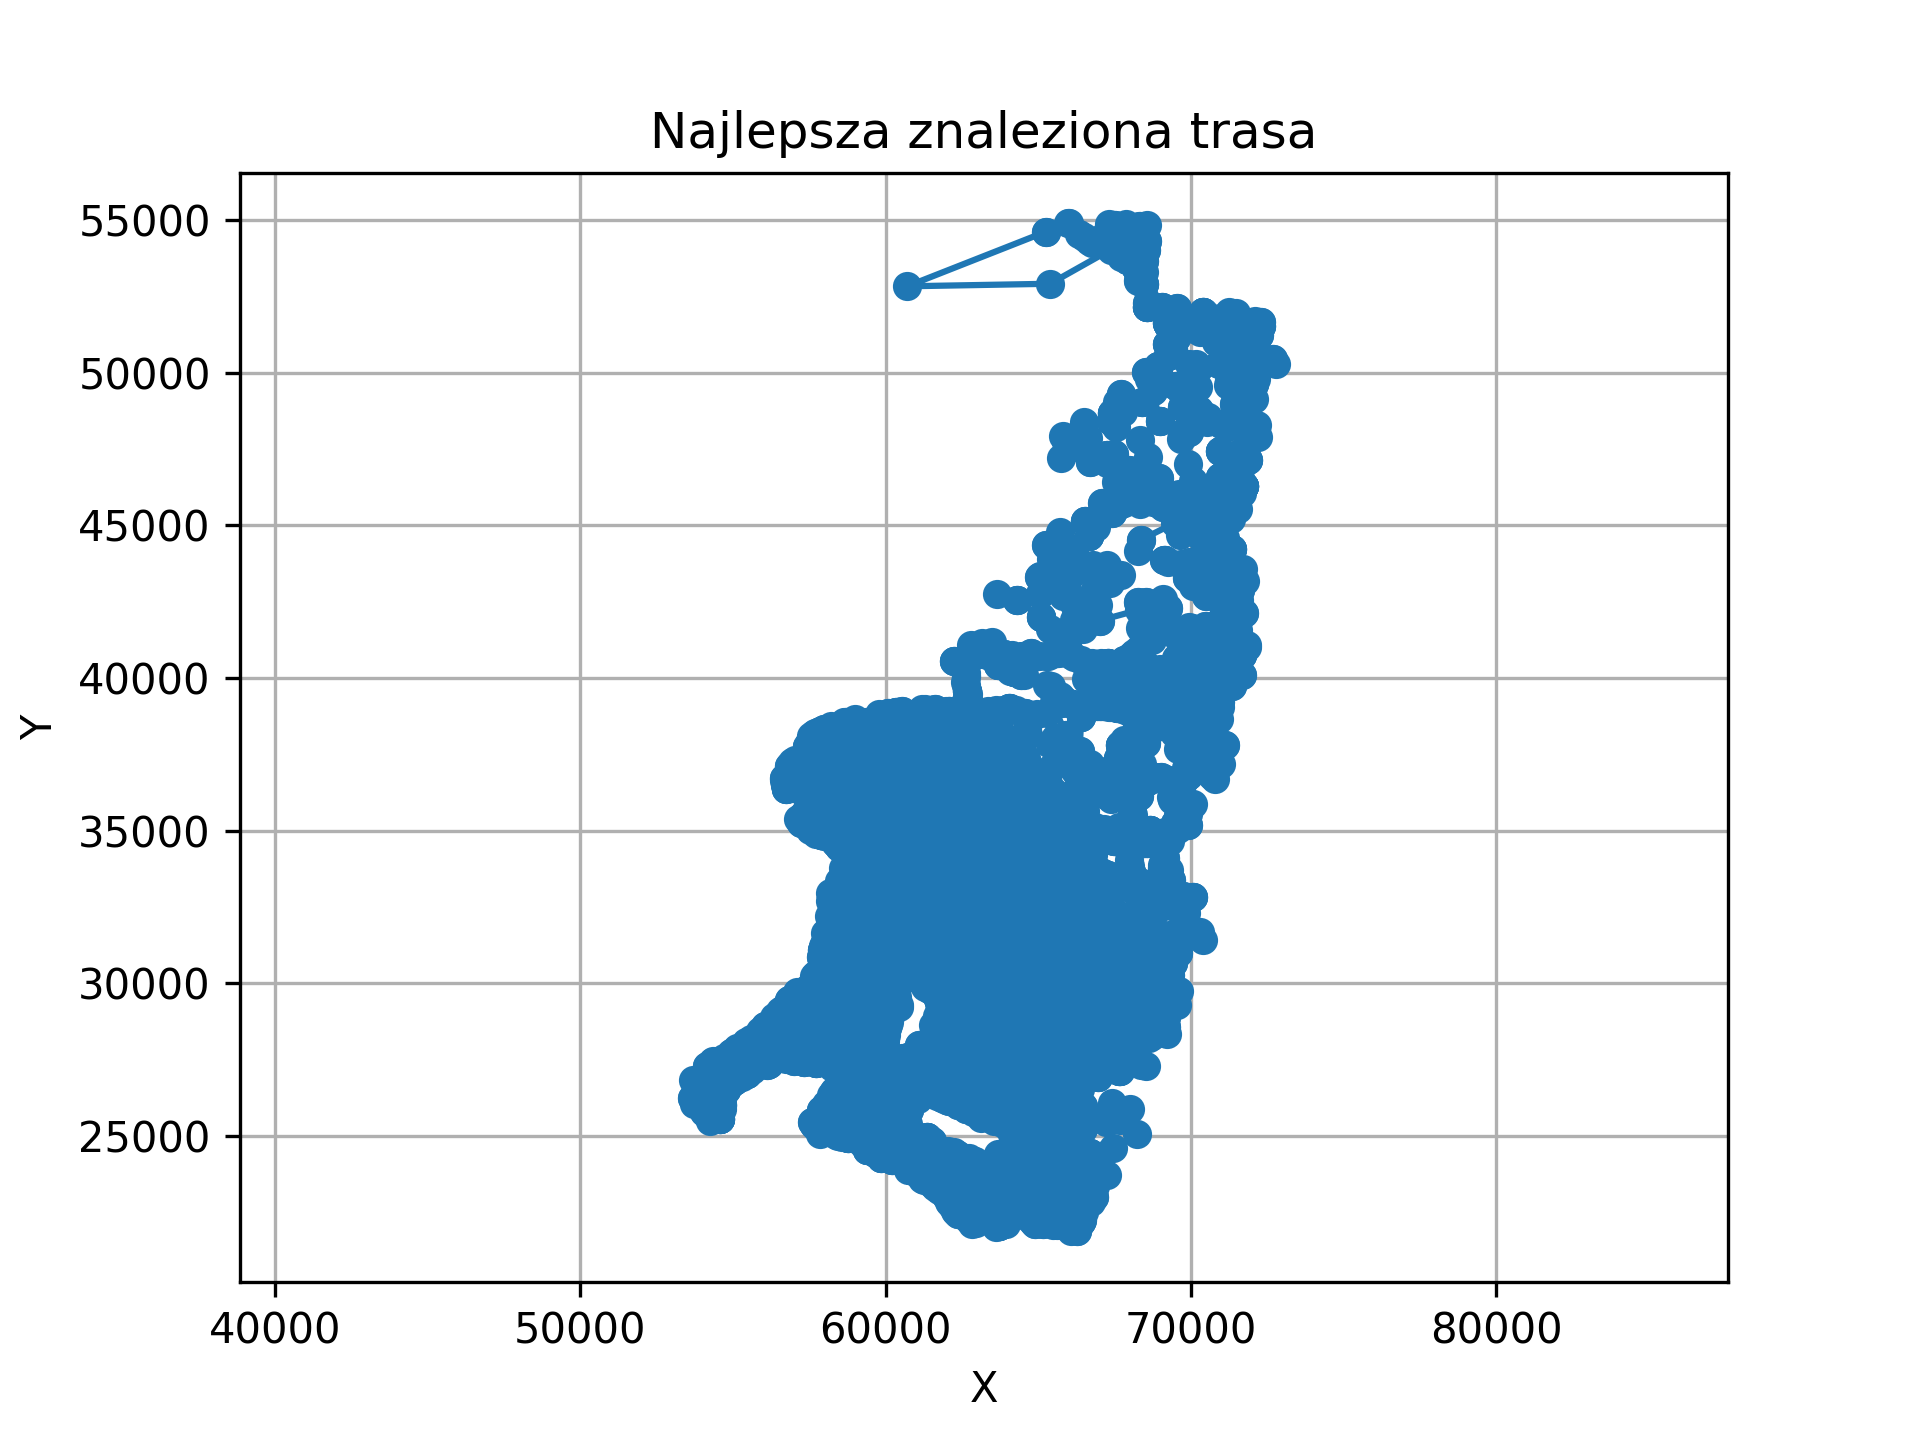
\includegraphics[width=0.8\textwidth]{best_route_ar9152.png}
    \caption{Najlepsza trasa znaleziona przez symulowane wyżarzanie dla instancji \texttt{ar9152.tsp}.}
\end{figure}

\subsubsection{Instancja \texttt{it16862.tsp}}

\begin{figure}[H]
    \centering
    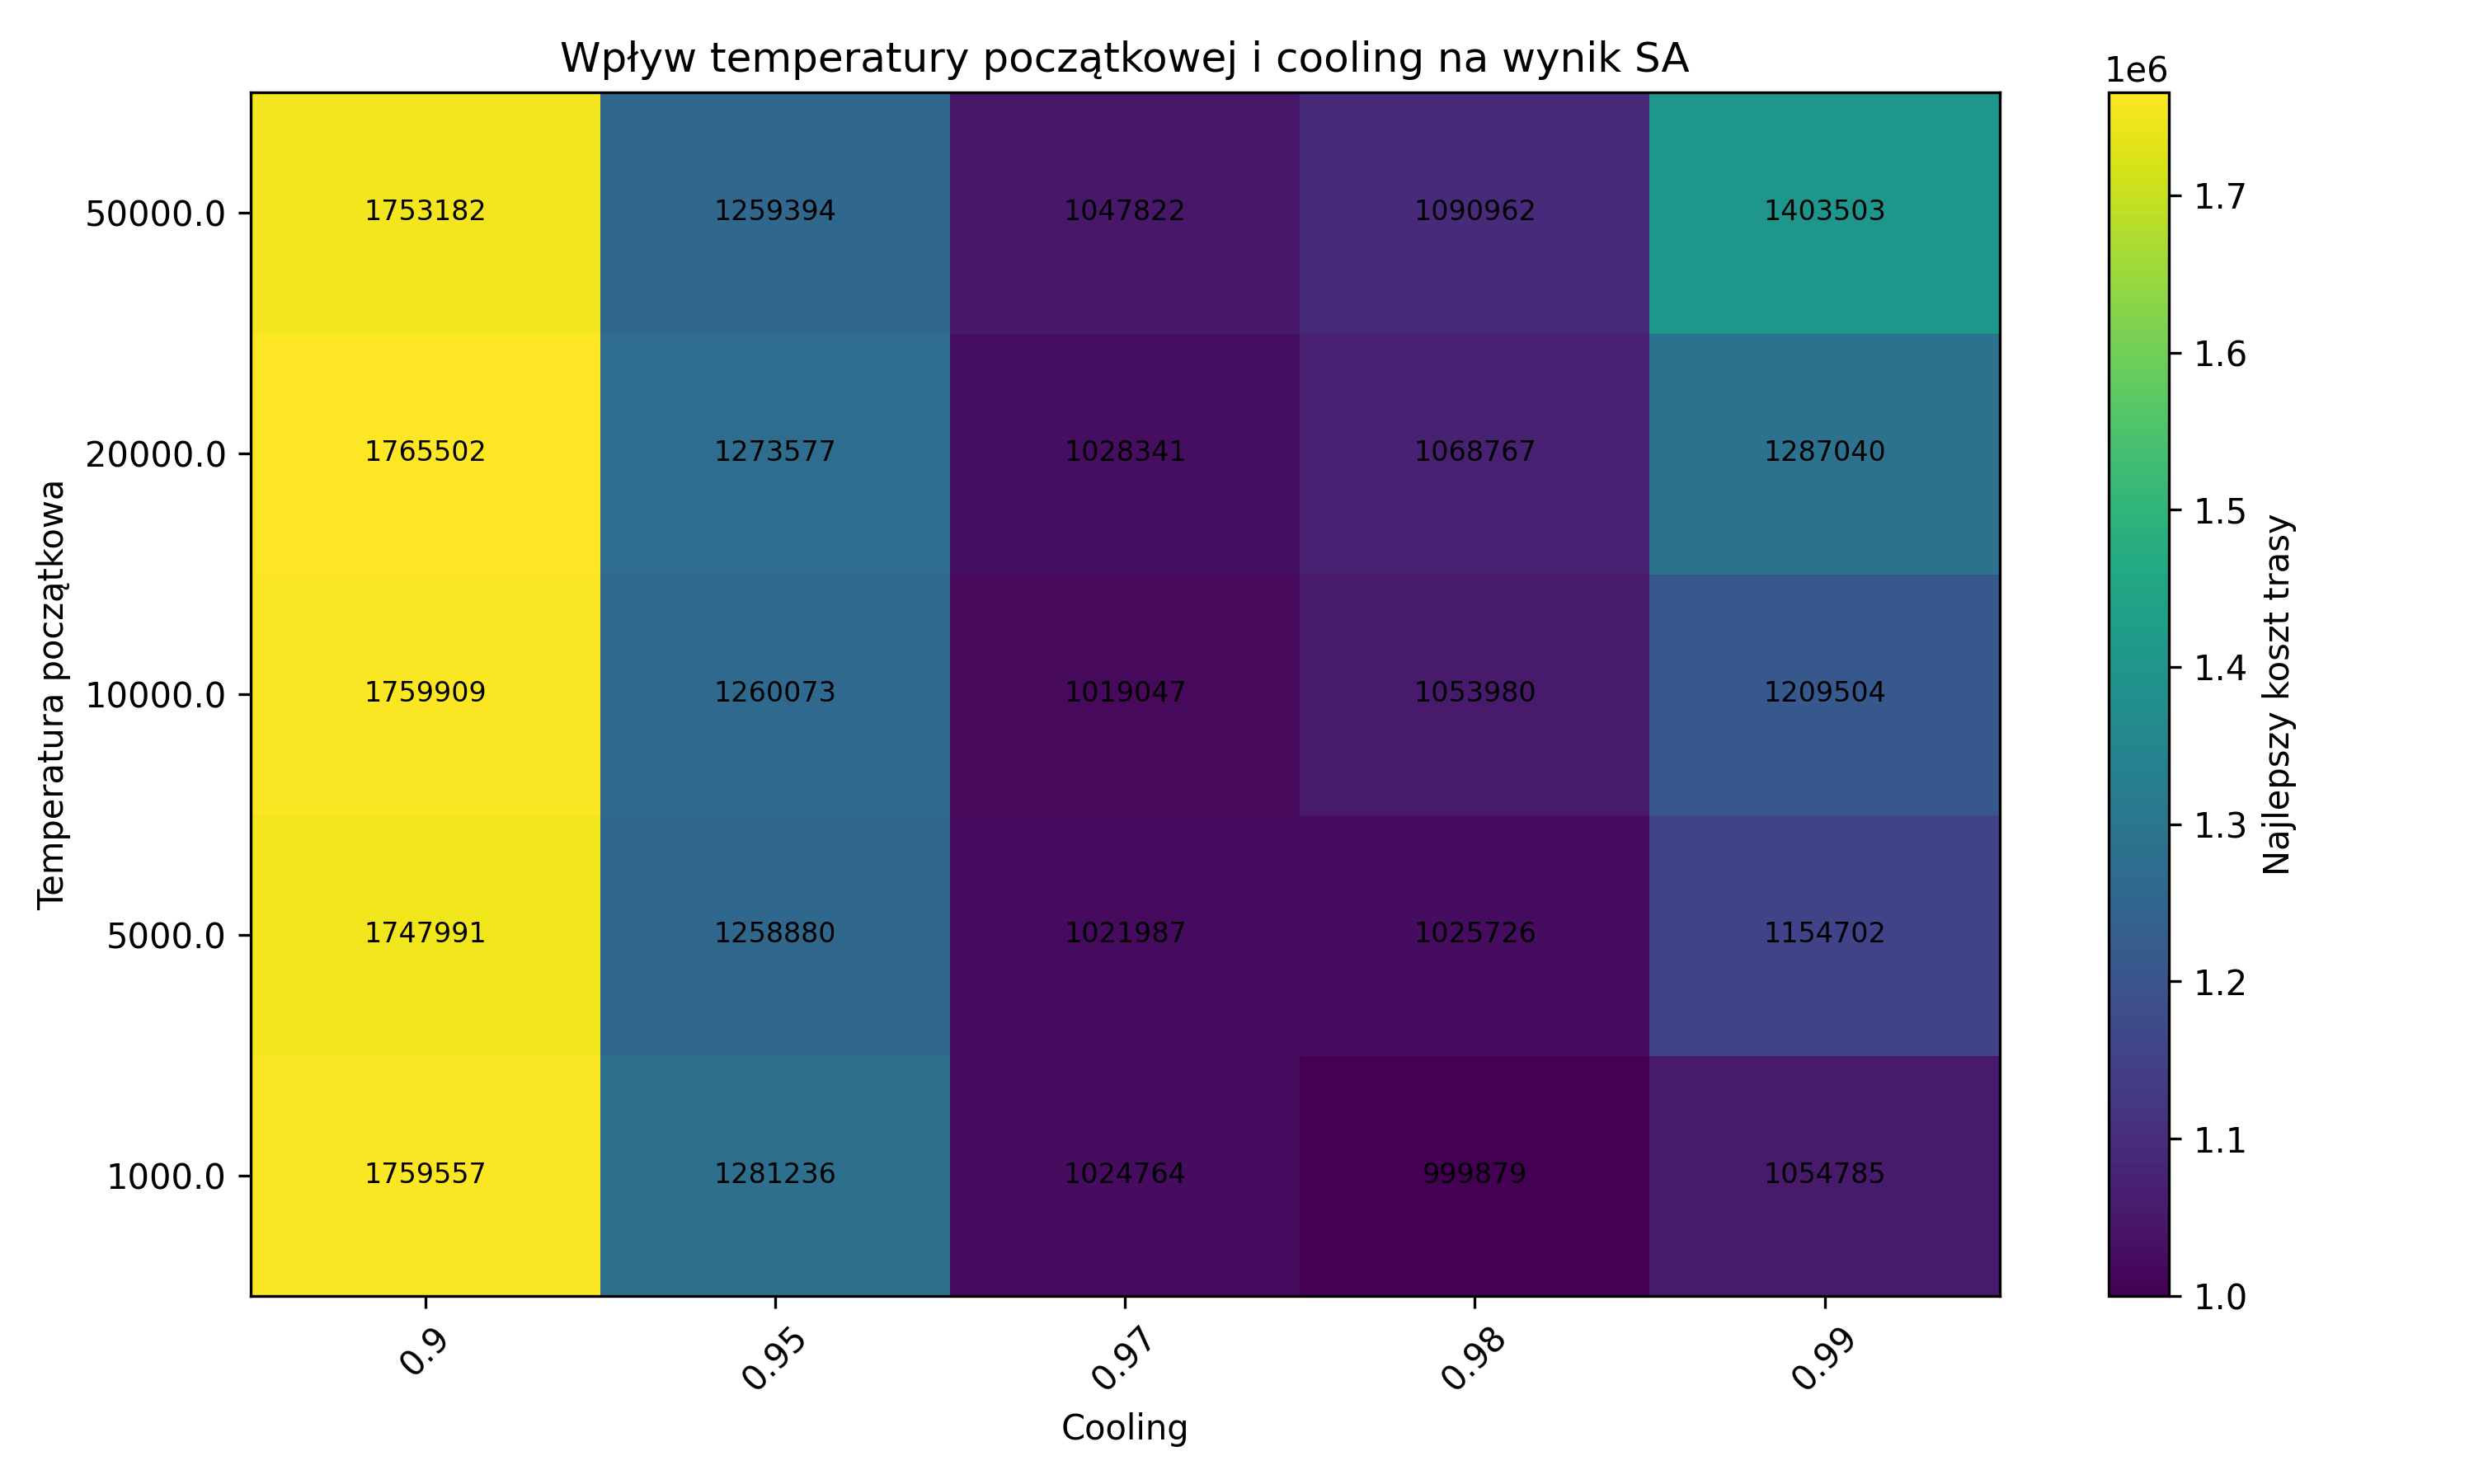
\includegraphics[width=0.9\textwidth]{temperature_grid_heatmap_it16862.png}
    \caption{Wpływ temperatury początkowej i współczynnika chłodzenia na wynik algorytmu symulowanego wyżarzania dla instancji \texttt{it16862.tsp}.}
\end{figure}

\begin{figure}[H]
    \centering
    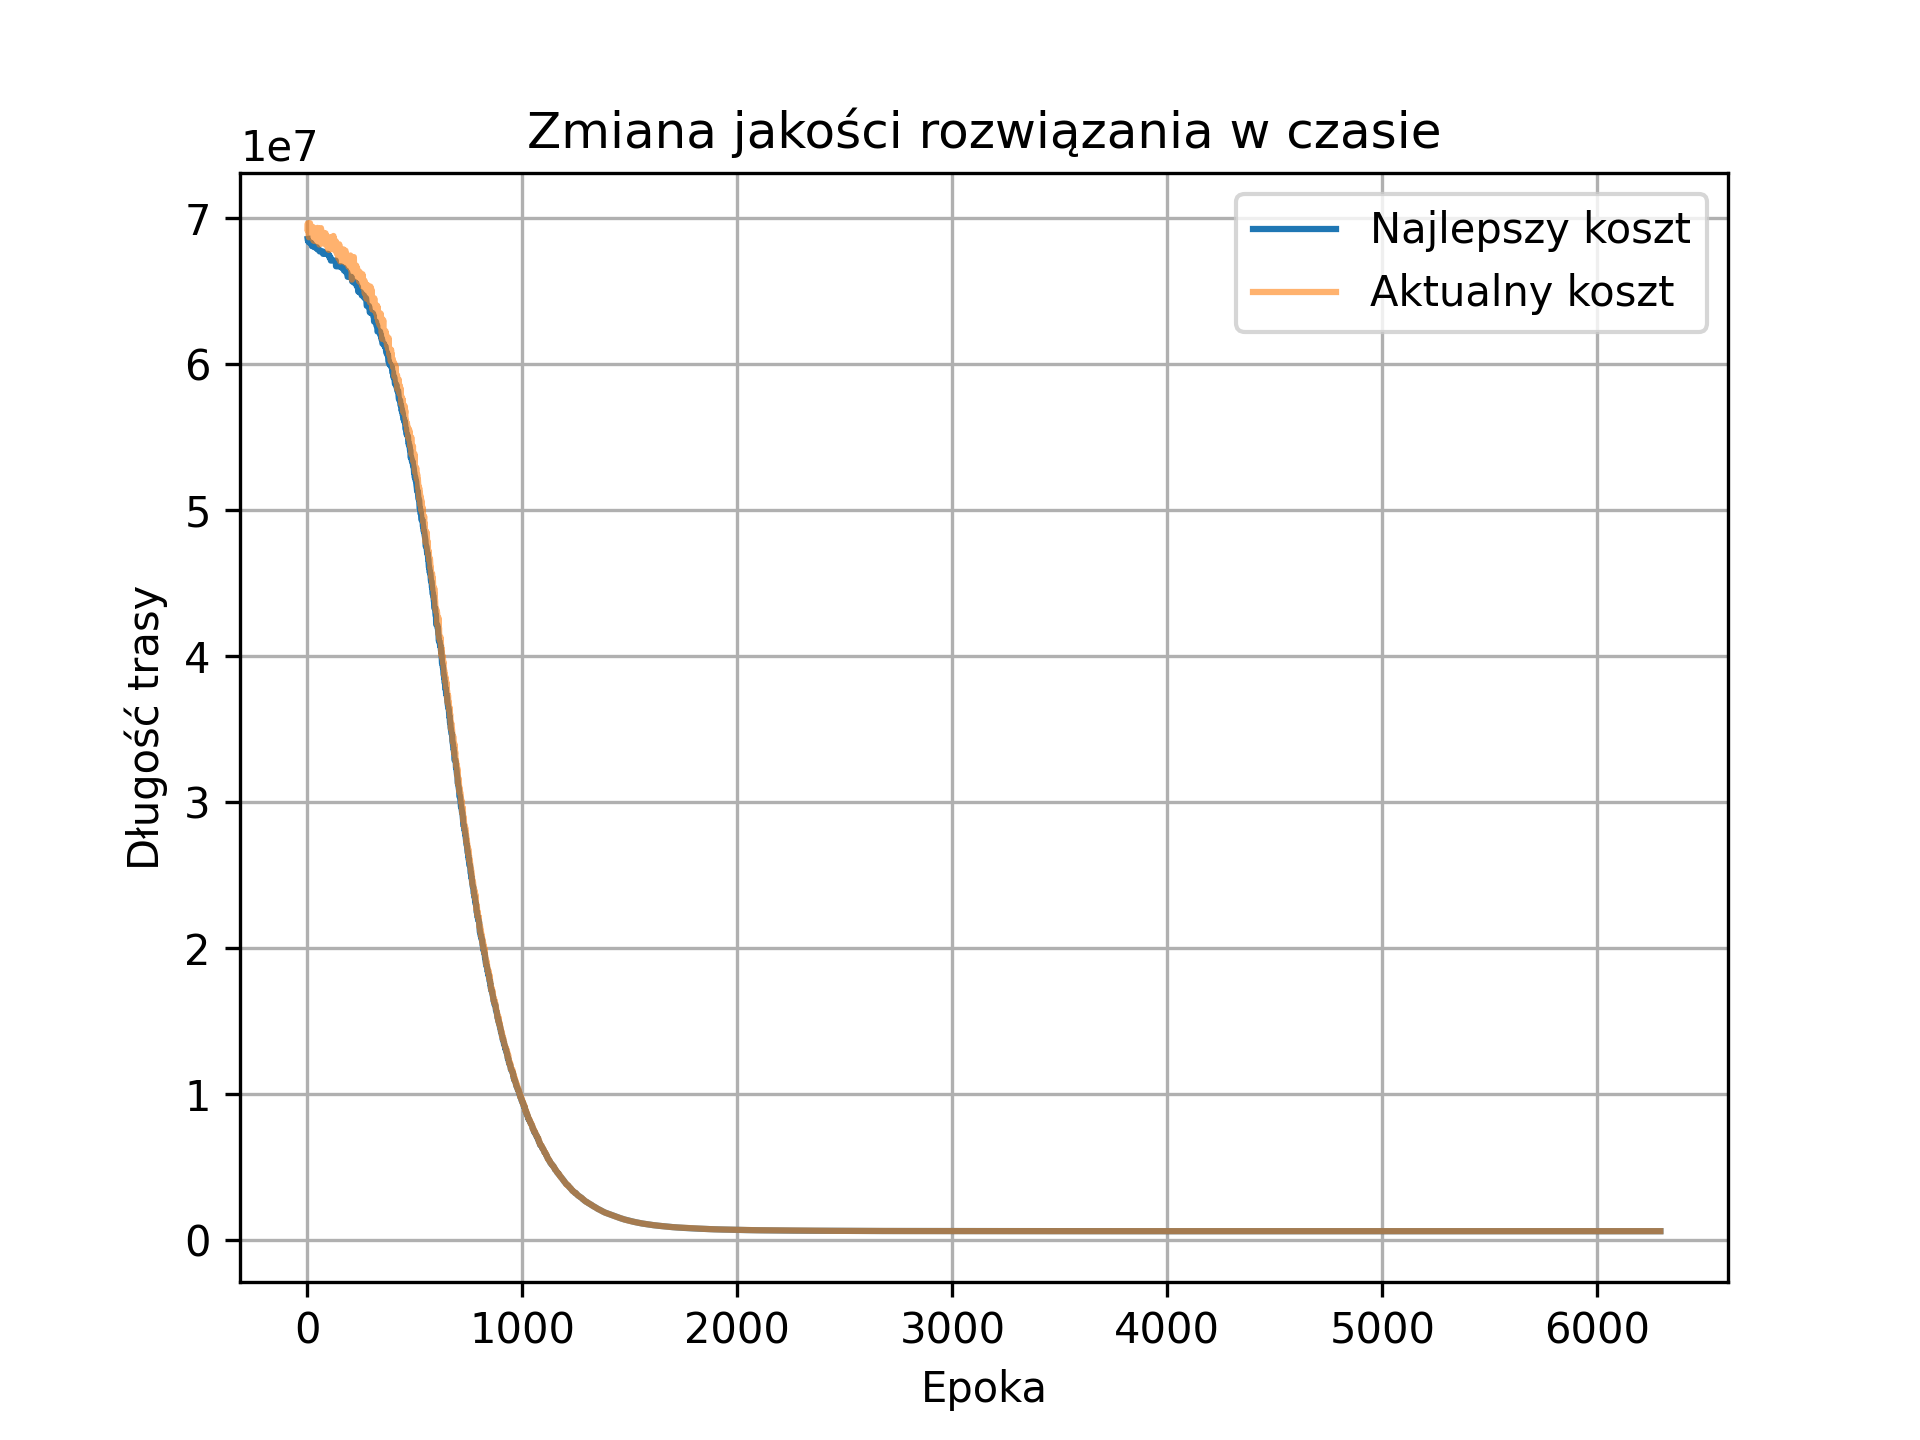
\includegraphics[width=0.9\textwidth]{cost_history_it16862.png}
    \caption{Zmiana najlepszego i aktualnego kosztu w czasie dla instancji \texttt{it16862.tsp}.}
\end{figure}

\begin{figure}[H]
    \centering
    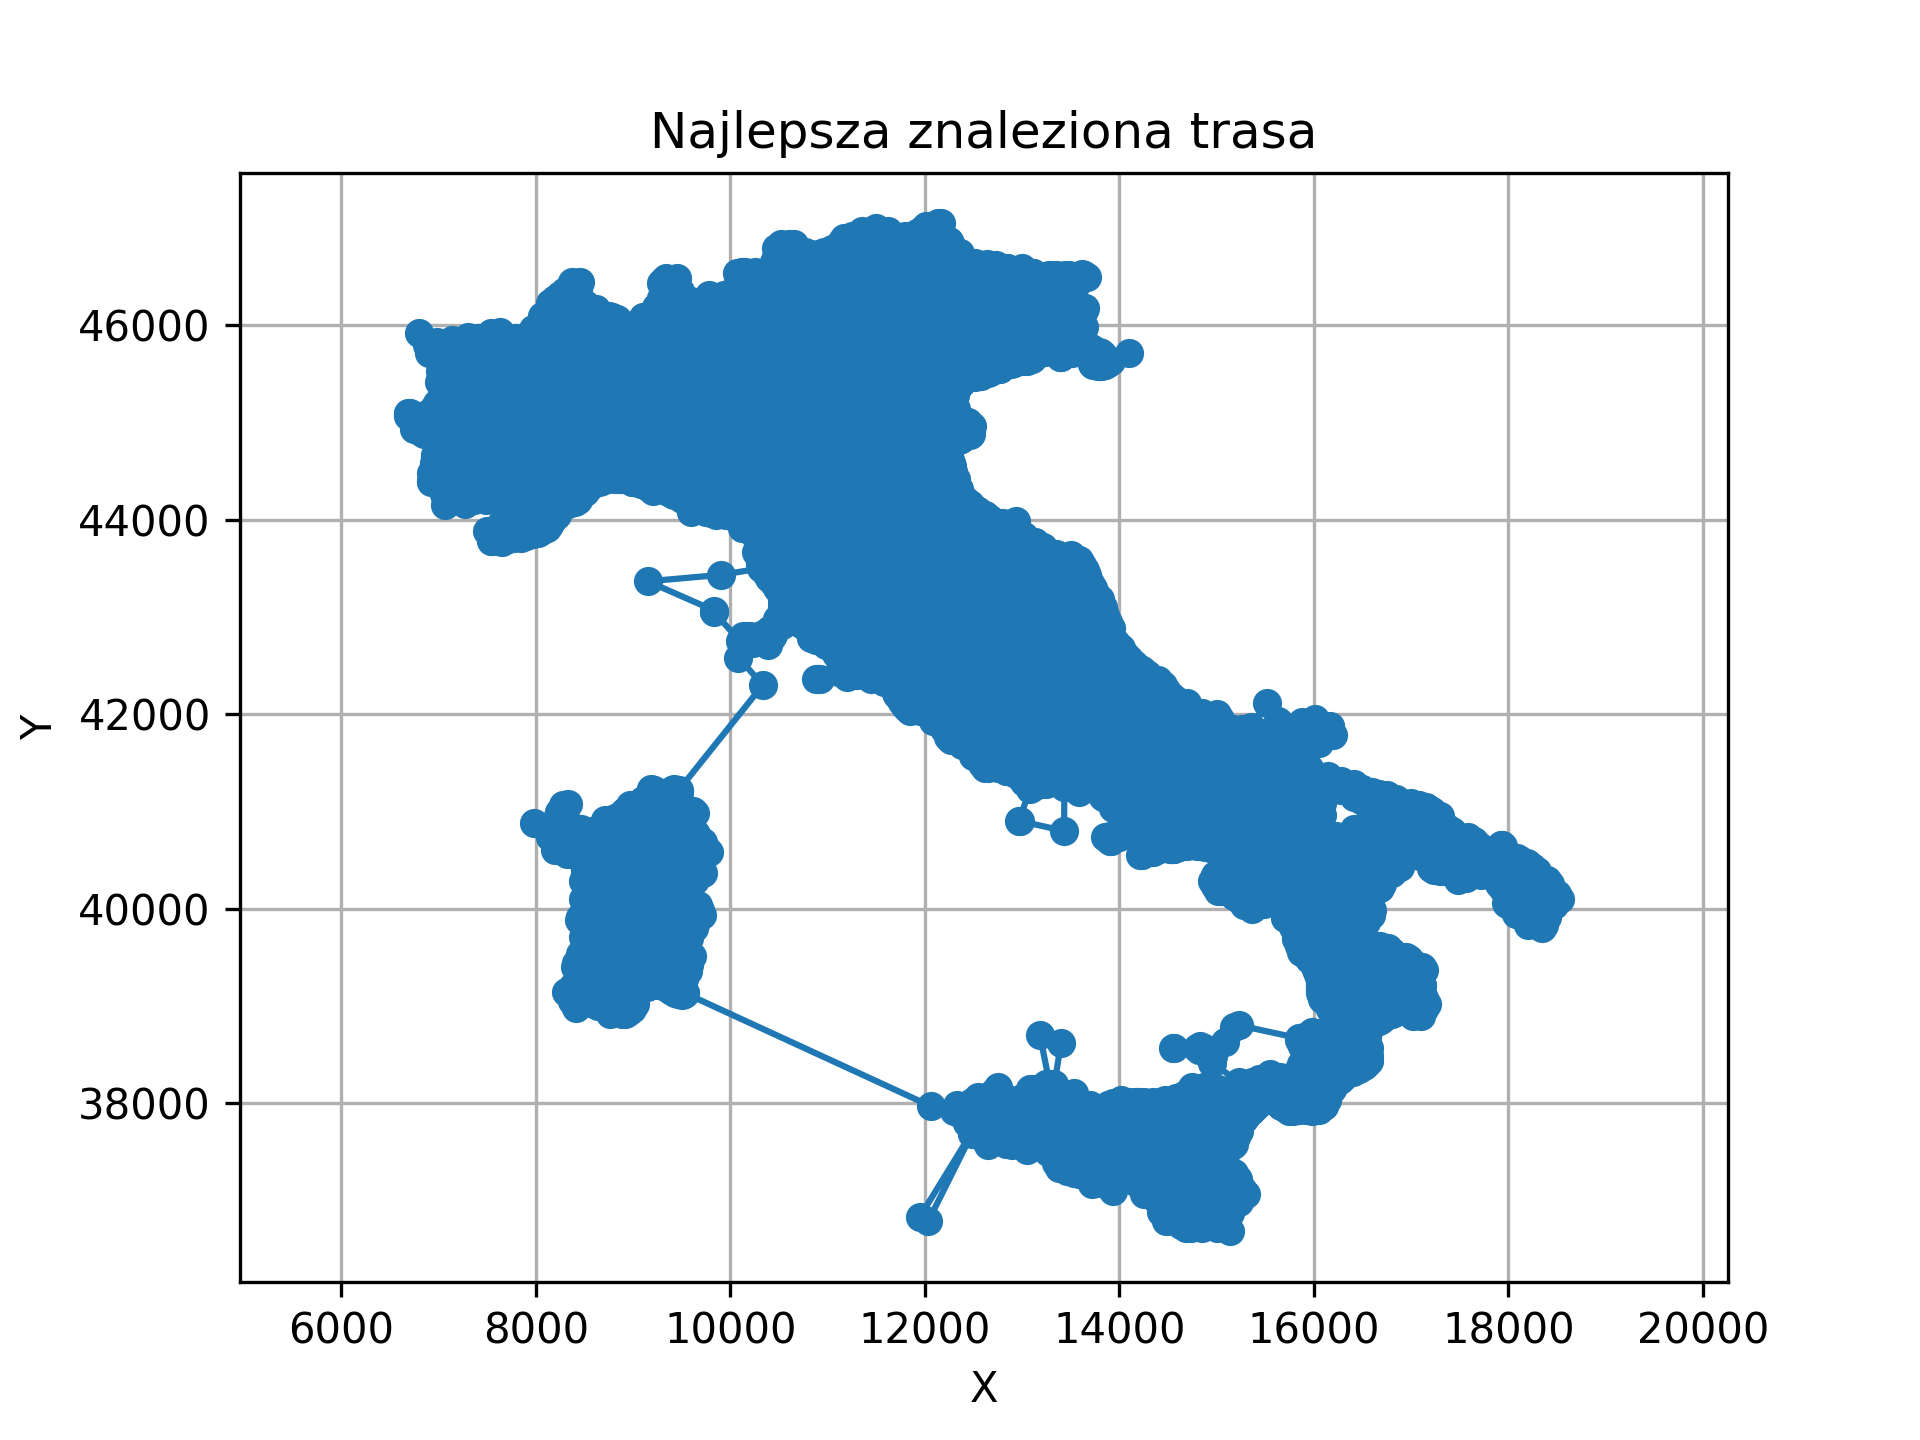
\includegraphics[width=0.8\textwidth]{best_route_it16862.png}
    \caption{Najlepsza trasa znaleziona przez symulowane wyżarzanie dla instancji \texttt{it16862.tsp}.}
\end{figure}

\subsection{Wyniki symulowanego wyżarzania}
\begin{table}[H]
    \centering
    \caption{Wyniki symulowanego wyżarzania dla wykonanych uruchomień.}
    \begin{tabular}{lrrrrr}
        \toprule
        Instancja & Najlepszy koszt & Best Bound & \% \\
        \midrule
        \texttt{eg7146.tsp}  & 182063.0000  & 172387 & 105.61\% \\
        \texttt{ar9152.tsp}  & 917262.0000  & 837479 & 109.53\% \\
        \texttt{it16862.tsp} & 624285.0000  & 557315 & 112.02\% \\
        \bottomrule 
    \end{tabular}
\end{table}

\section{Tabu Search}

\subsection{Opis metody}

Tabu Search jest rozszerzeniem lokalnego przeszukiwania. Klasyczne lokalne przeszukiwanie może łatwo utknąć w minimum lokalnym, ponieważ akceptuje tylko ruchy poprawiające rozwiązanie. Tabu Search umożliwia wykonanie również ruchów pogarszających, ale jednocześnie zapobiega cyklicznemu powracaniu do tych samych rozwiązań przez zastosowanie listy tabu.

W implementacji na liście tabu przechowywano wykonane ruchy \texttt{2-opt}, reprezentowane przez parę indeksów $(i,j)$. Po wykonaniu ruchu był on zabroniony przez określoną liczbę iteracji, zadaną parametrem \texttt{tabuTenure}.

\subsection{Zastosowane parametry}

Program umożliwiał zmianę parametrów:

\begin{itemize}
    \item \texttt{--iterations} -- maksymalna liczba iteracji,
    \item \texttt{--no-improve} -- limit iteracji bez poprawy,
    \item \texttt{--tabu} -- długość listy tabu,
    \item \texttt{--sample} -- rozmiar losowej próbki sąsiedztwa,
\end{itemize}

\subsection{Dobór parametrów Tabu Search}

Długość listy tabu dobrano eksperymentalnie. Zbyt krótka lista tabu powodowała częste powracanie do wcześniej odwiedzonych obszarów przestrzeni rozwiązań. Zbyt długa lista tabu nadmiernie ograniczała dostępne ruchy i mogła pogarszać jakość przeszukiwania.

Dla dużych instancji zastosowano losowe próbkowanie sąsiedztwa. Parametr \texttt{sample} kontrolował kompromis pomiędzy czasem działania a jakością wyboru najlepszego ruchu. Większa próbka zwiększała szansę znalezienia lepszego ruchu w danej iteracji, ale wydłużała czas działania programu.

\subsection{Wykresy dla Tabu Search}

\subsubsection{Instancja \texttt{eg7146.tsp}}

\begin{figure}[H]
    \centering
    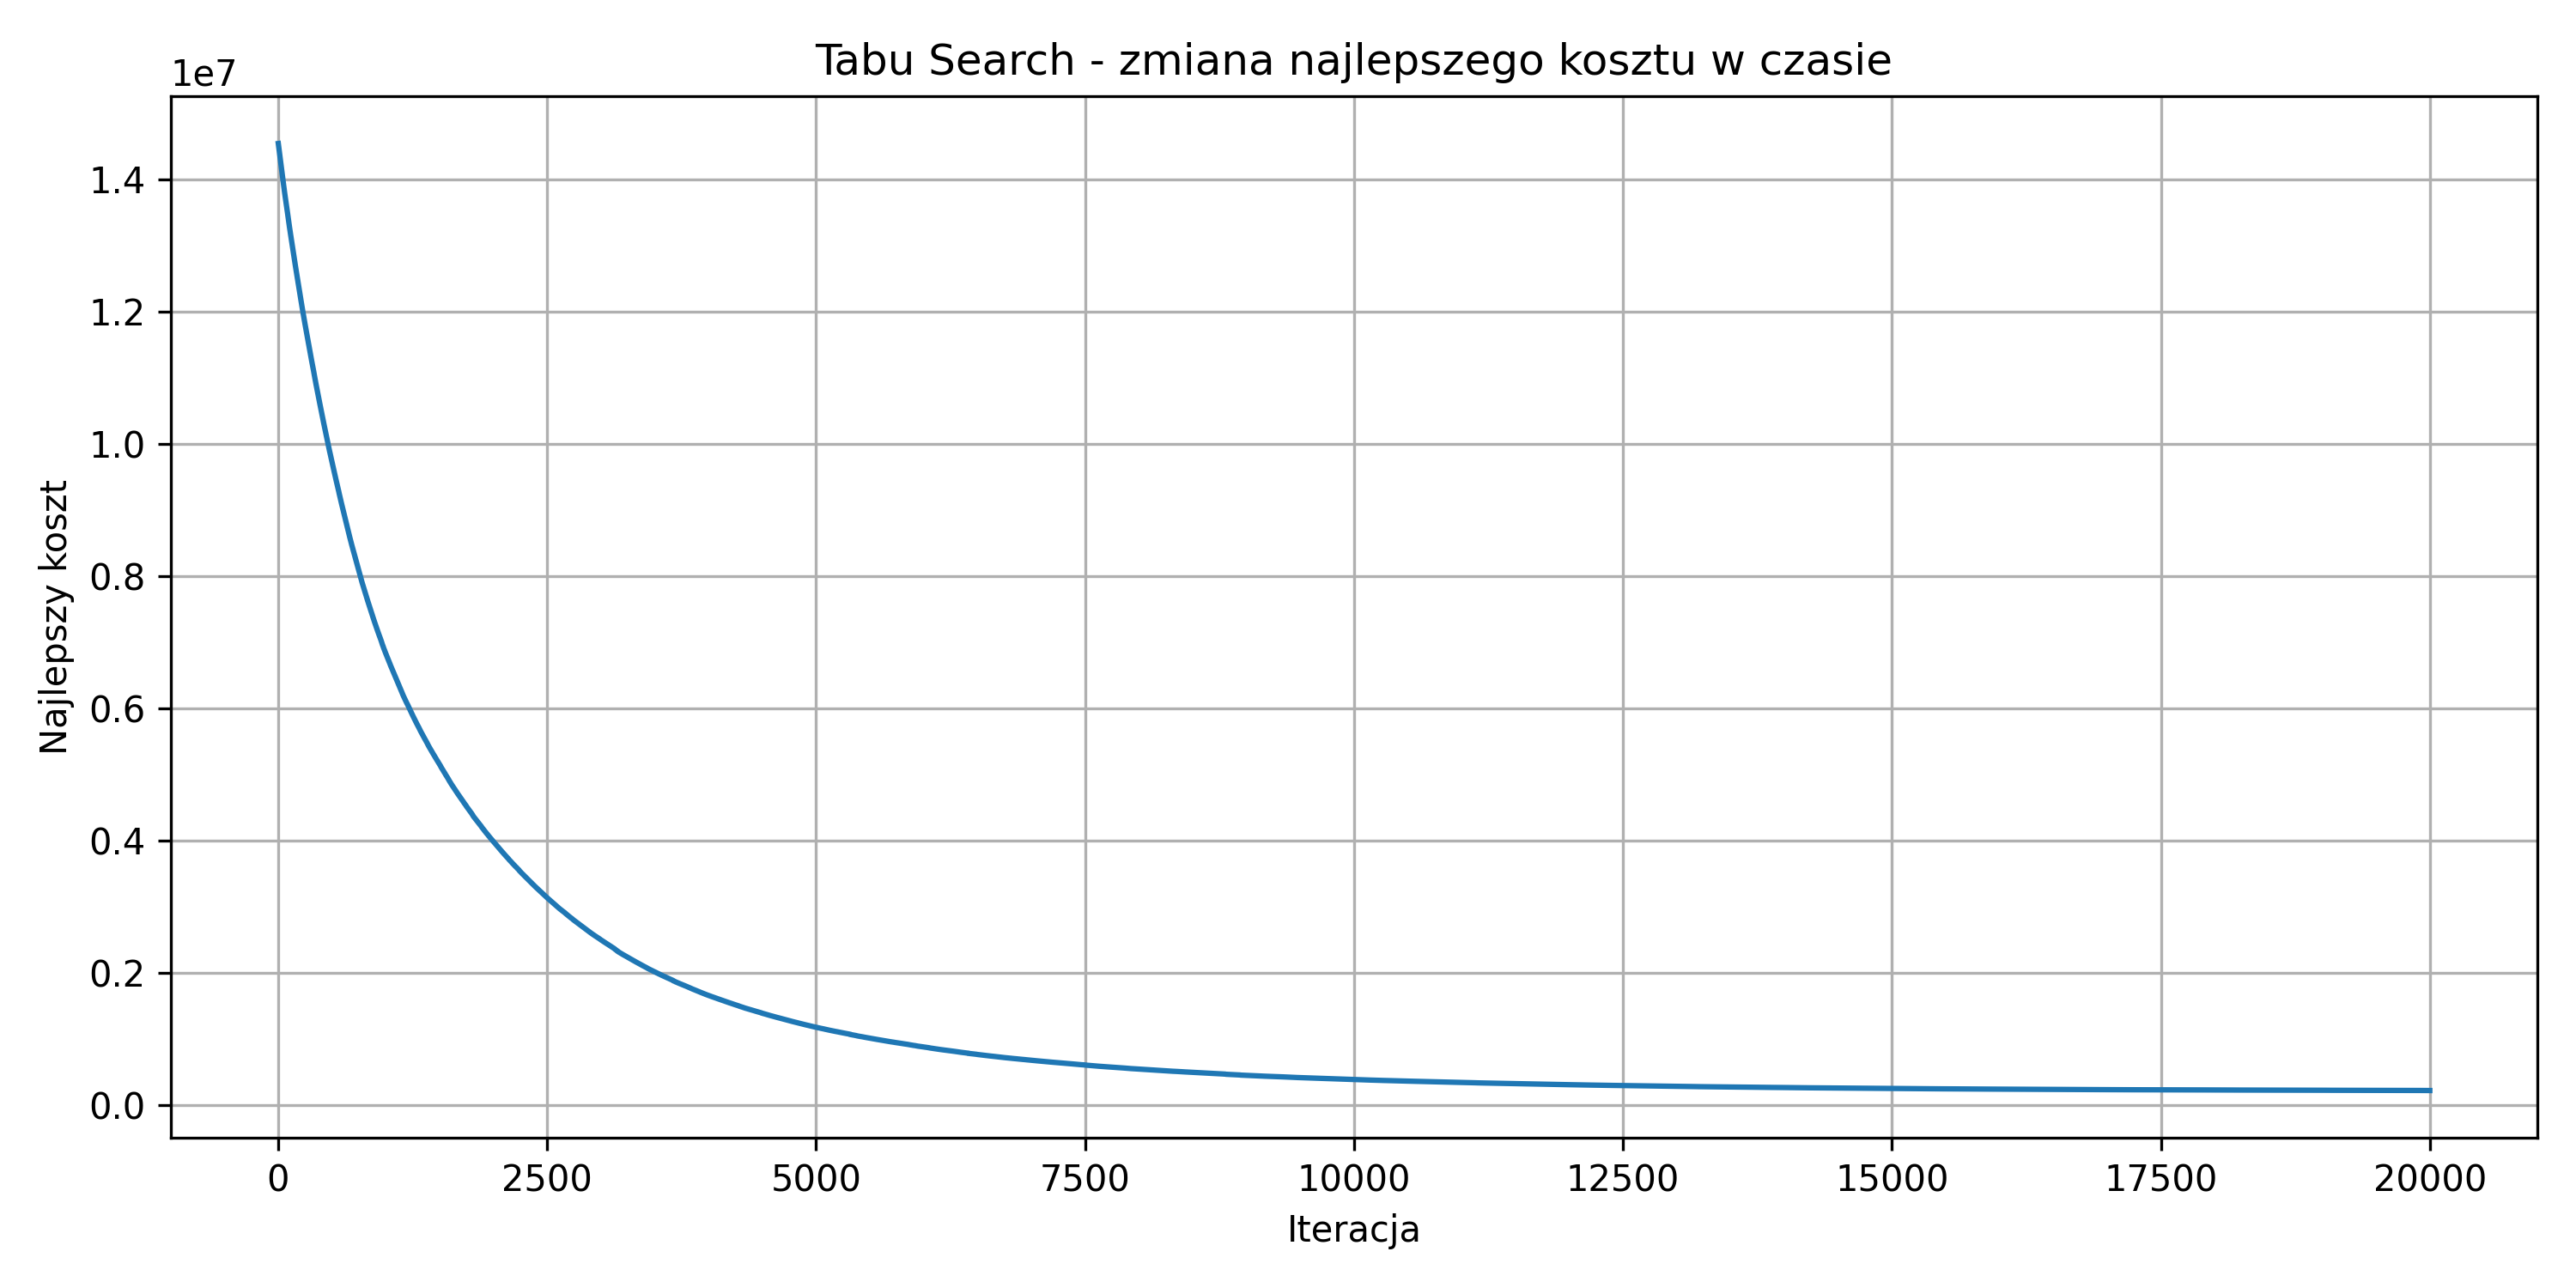
\includegraphics[width=0.9\textwidth]{tabu/tabu_history_eg7146.png}
    \caption{Zmiana najlepszego kosztu w kolejnych iteracjach Tabu Search dla instancji \texttt{eg7146.tsp}.}
\end{figure}

\begin{figure}[H]
    \centering
    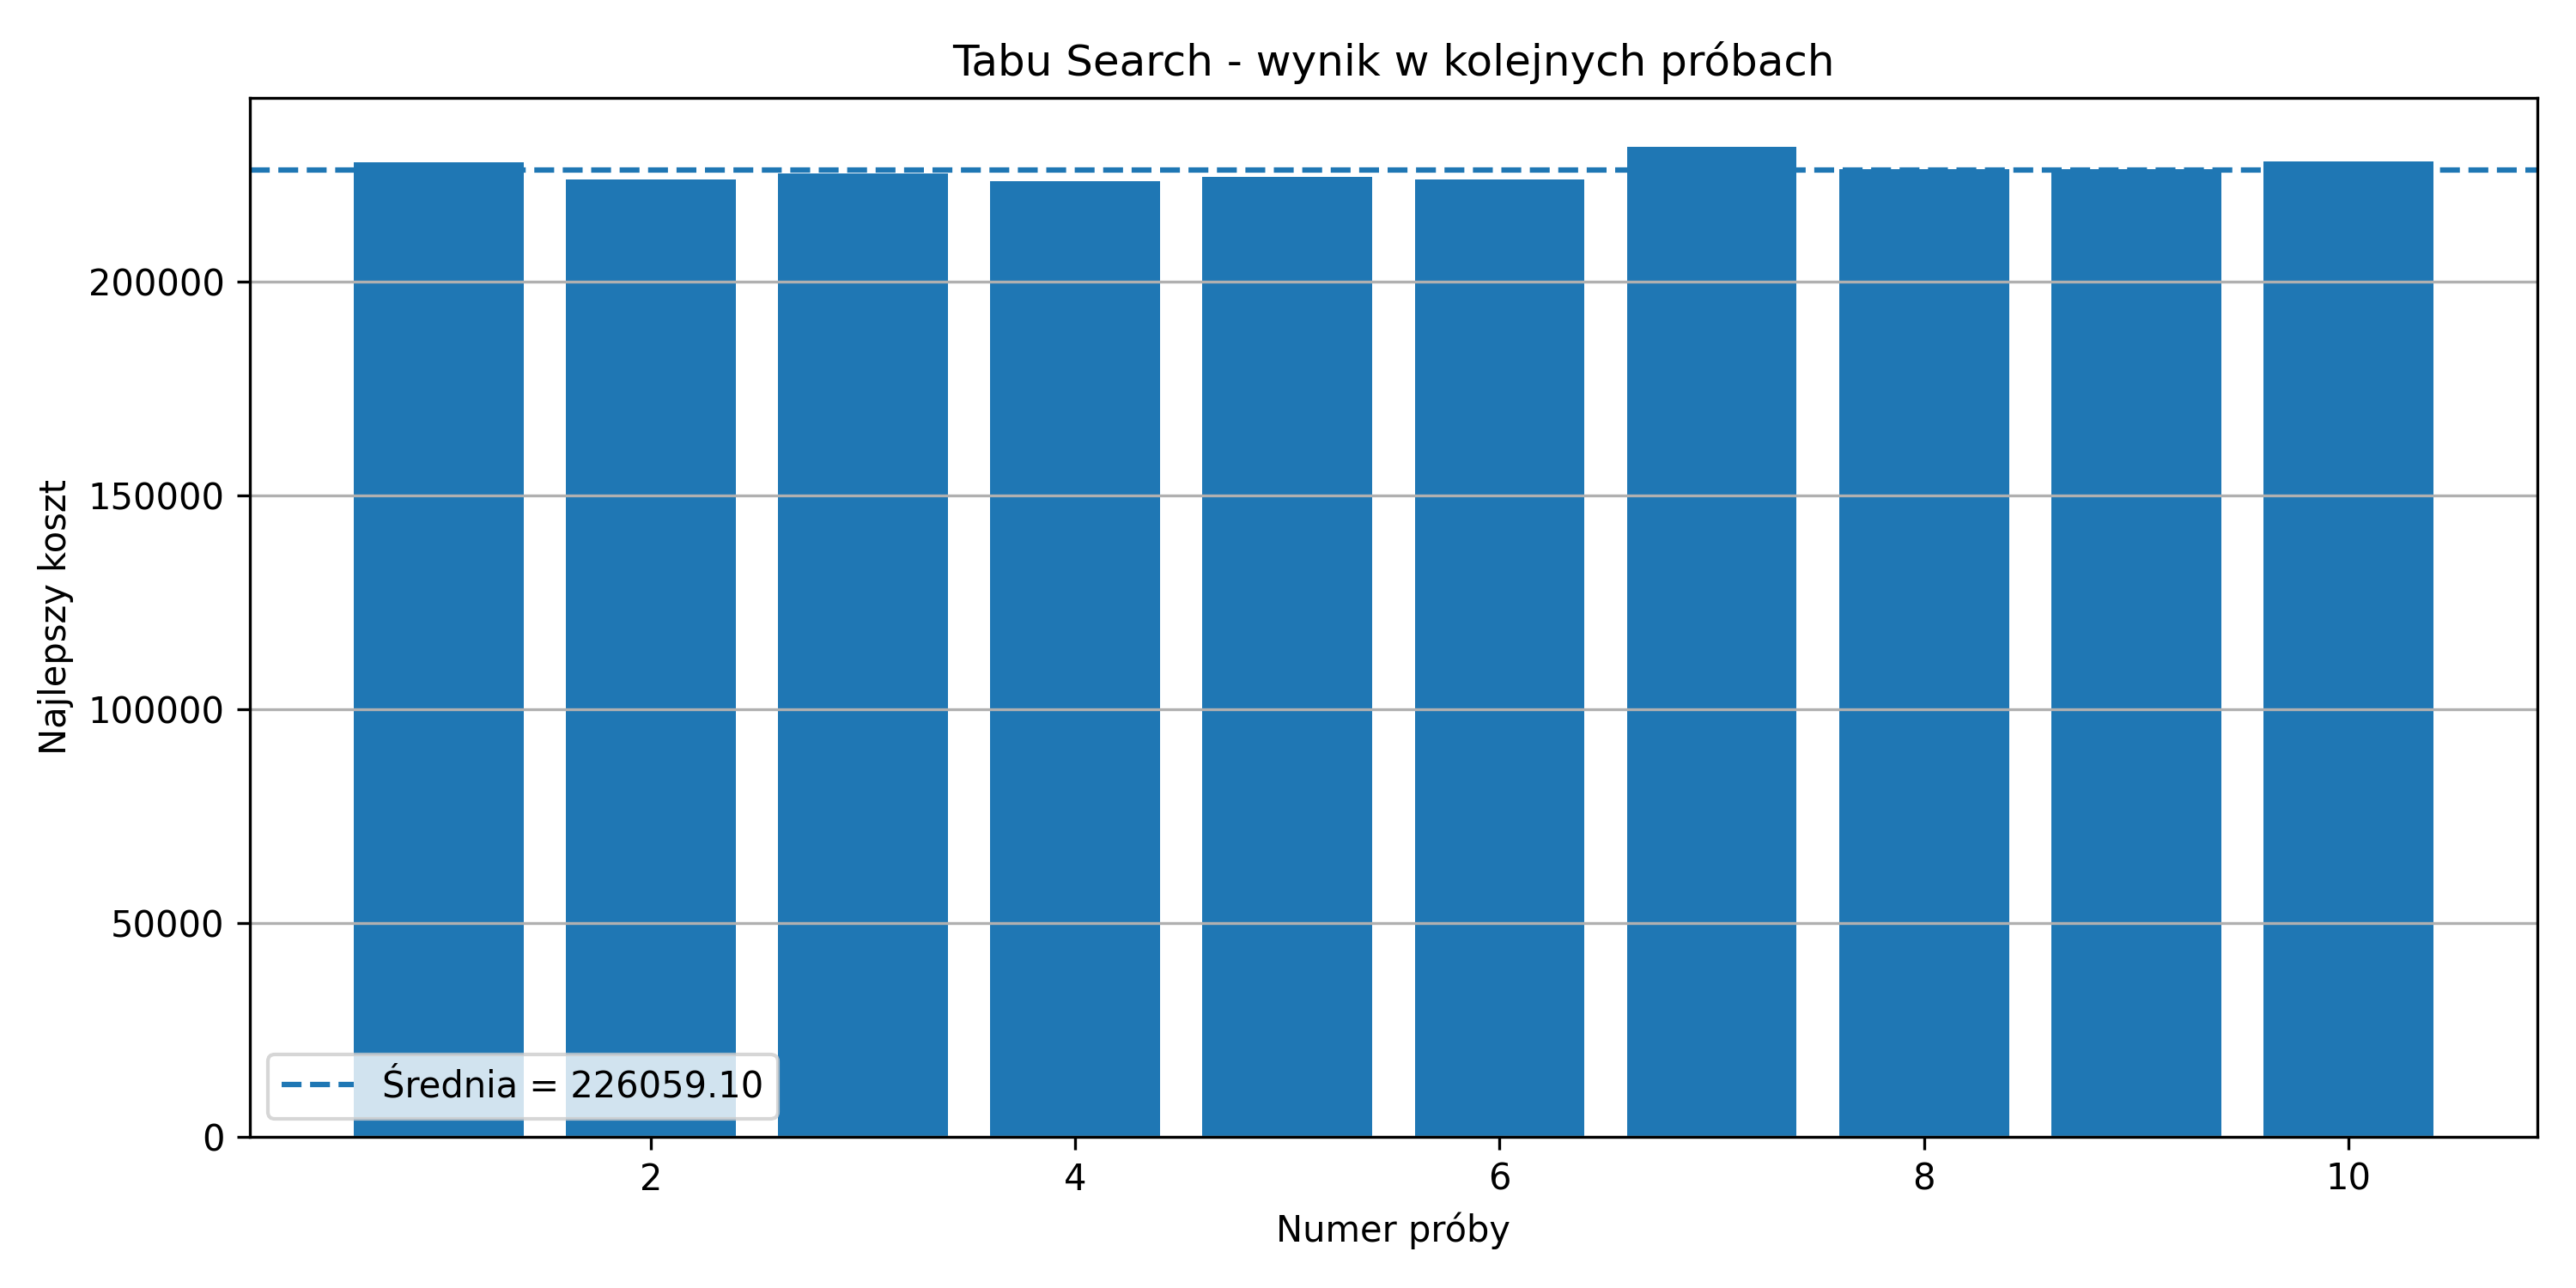
\includegraphics[width=0.9\textwidth]{tabu/tabu_runs_bar_eg7146.png}
    \caption{Najlepsze wyniki uzyskane w kolejnych próbach Tabu Search dla instancji \texttt{eg7146.tsp}.}
\end{figure}

\begin{figure}[H]
    \centering
    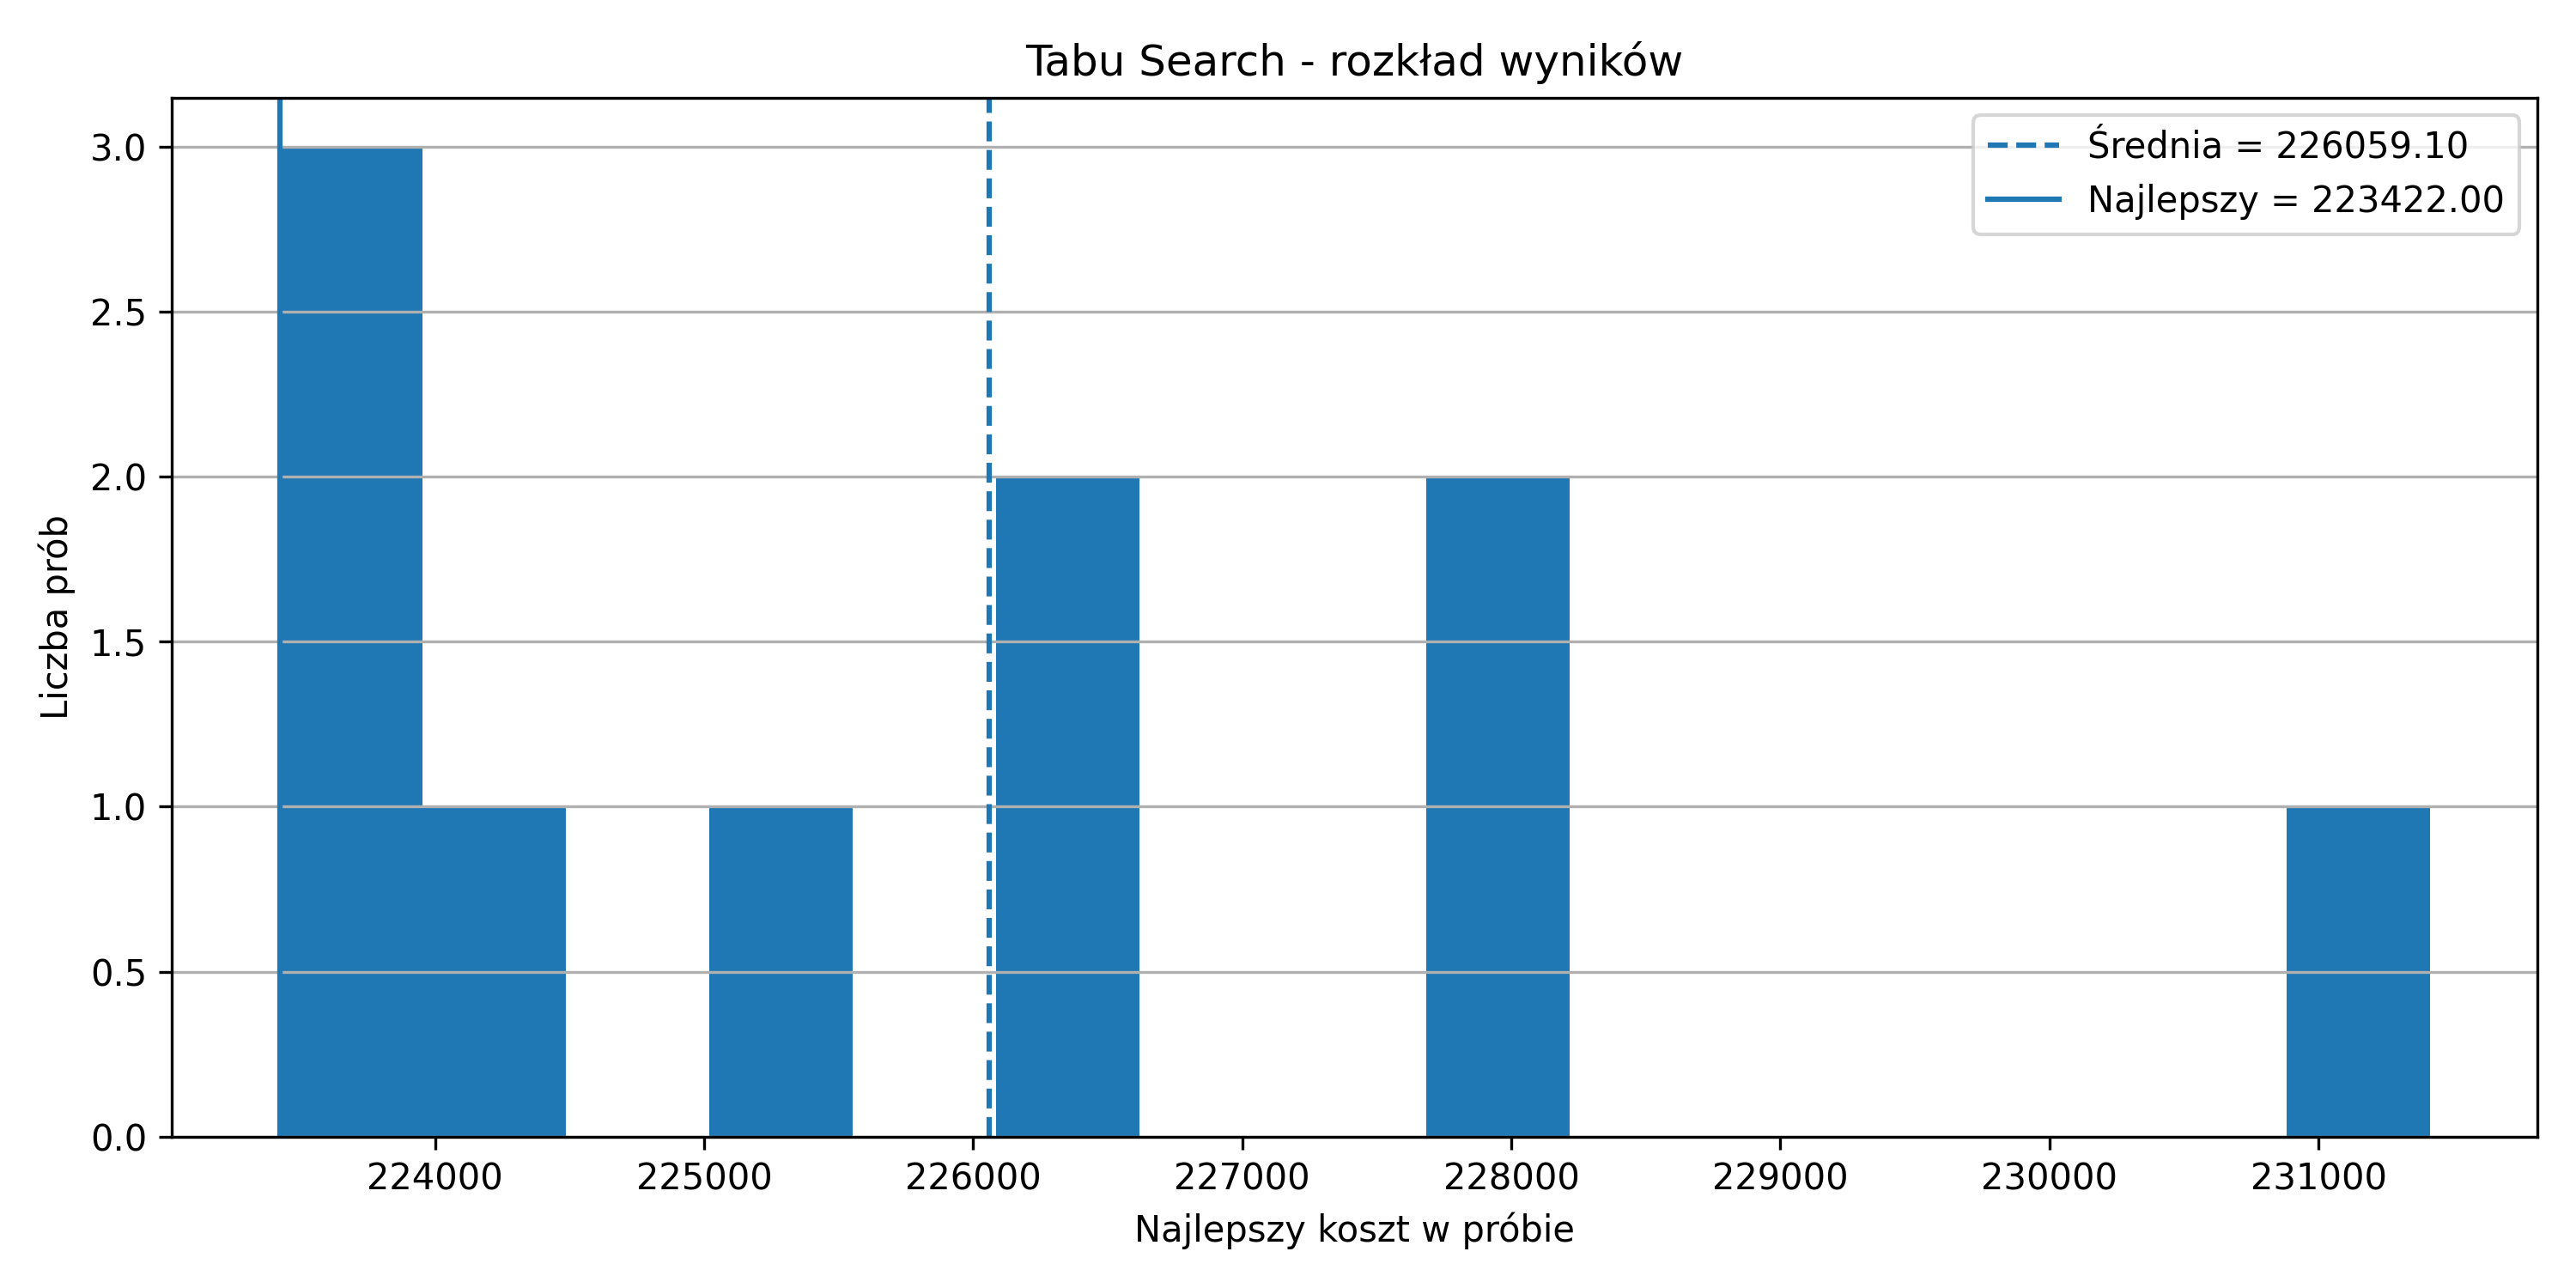
\includegraphics[width=0.9\textwidth]{tabu/tabu_runs_histogram_eg7146.png}
    \caption{Rozkład wyników uzyskanych w próbach Tabu Search dla instancji \texttt{eg7146.tsp}.}
\end{figure}

\begin{figure}[H]
    \centering
    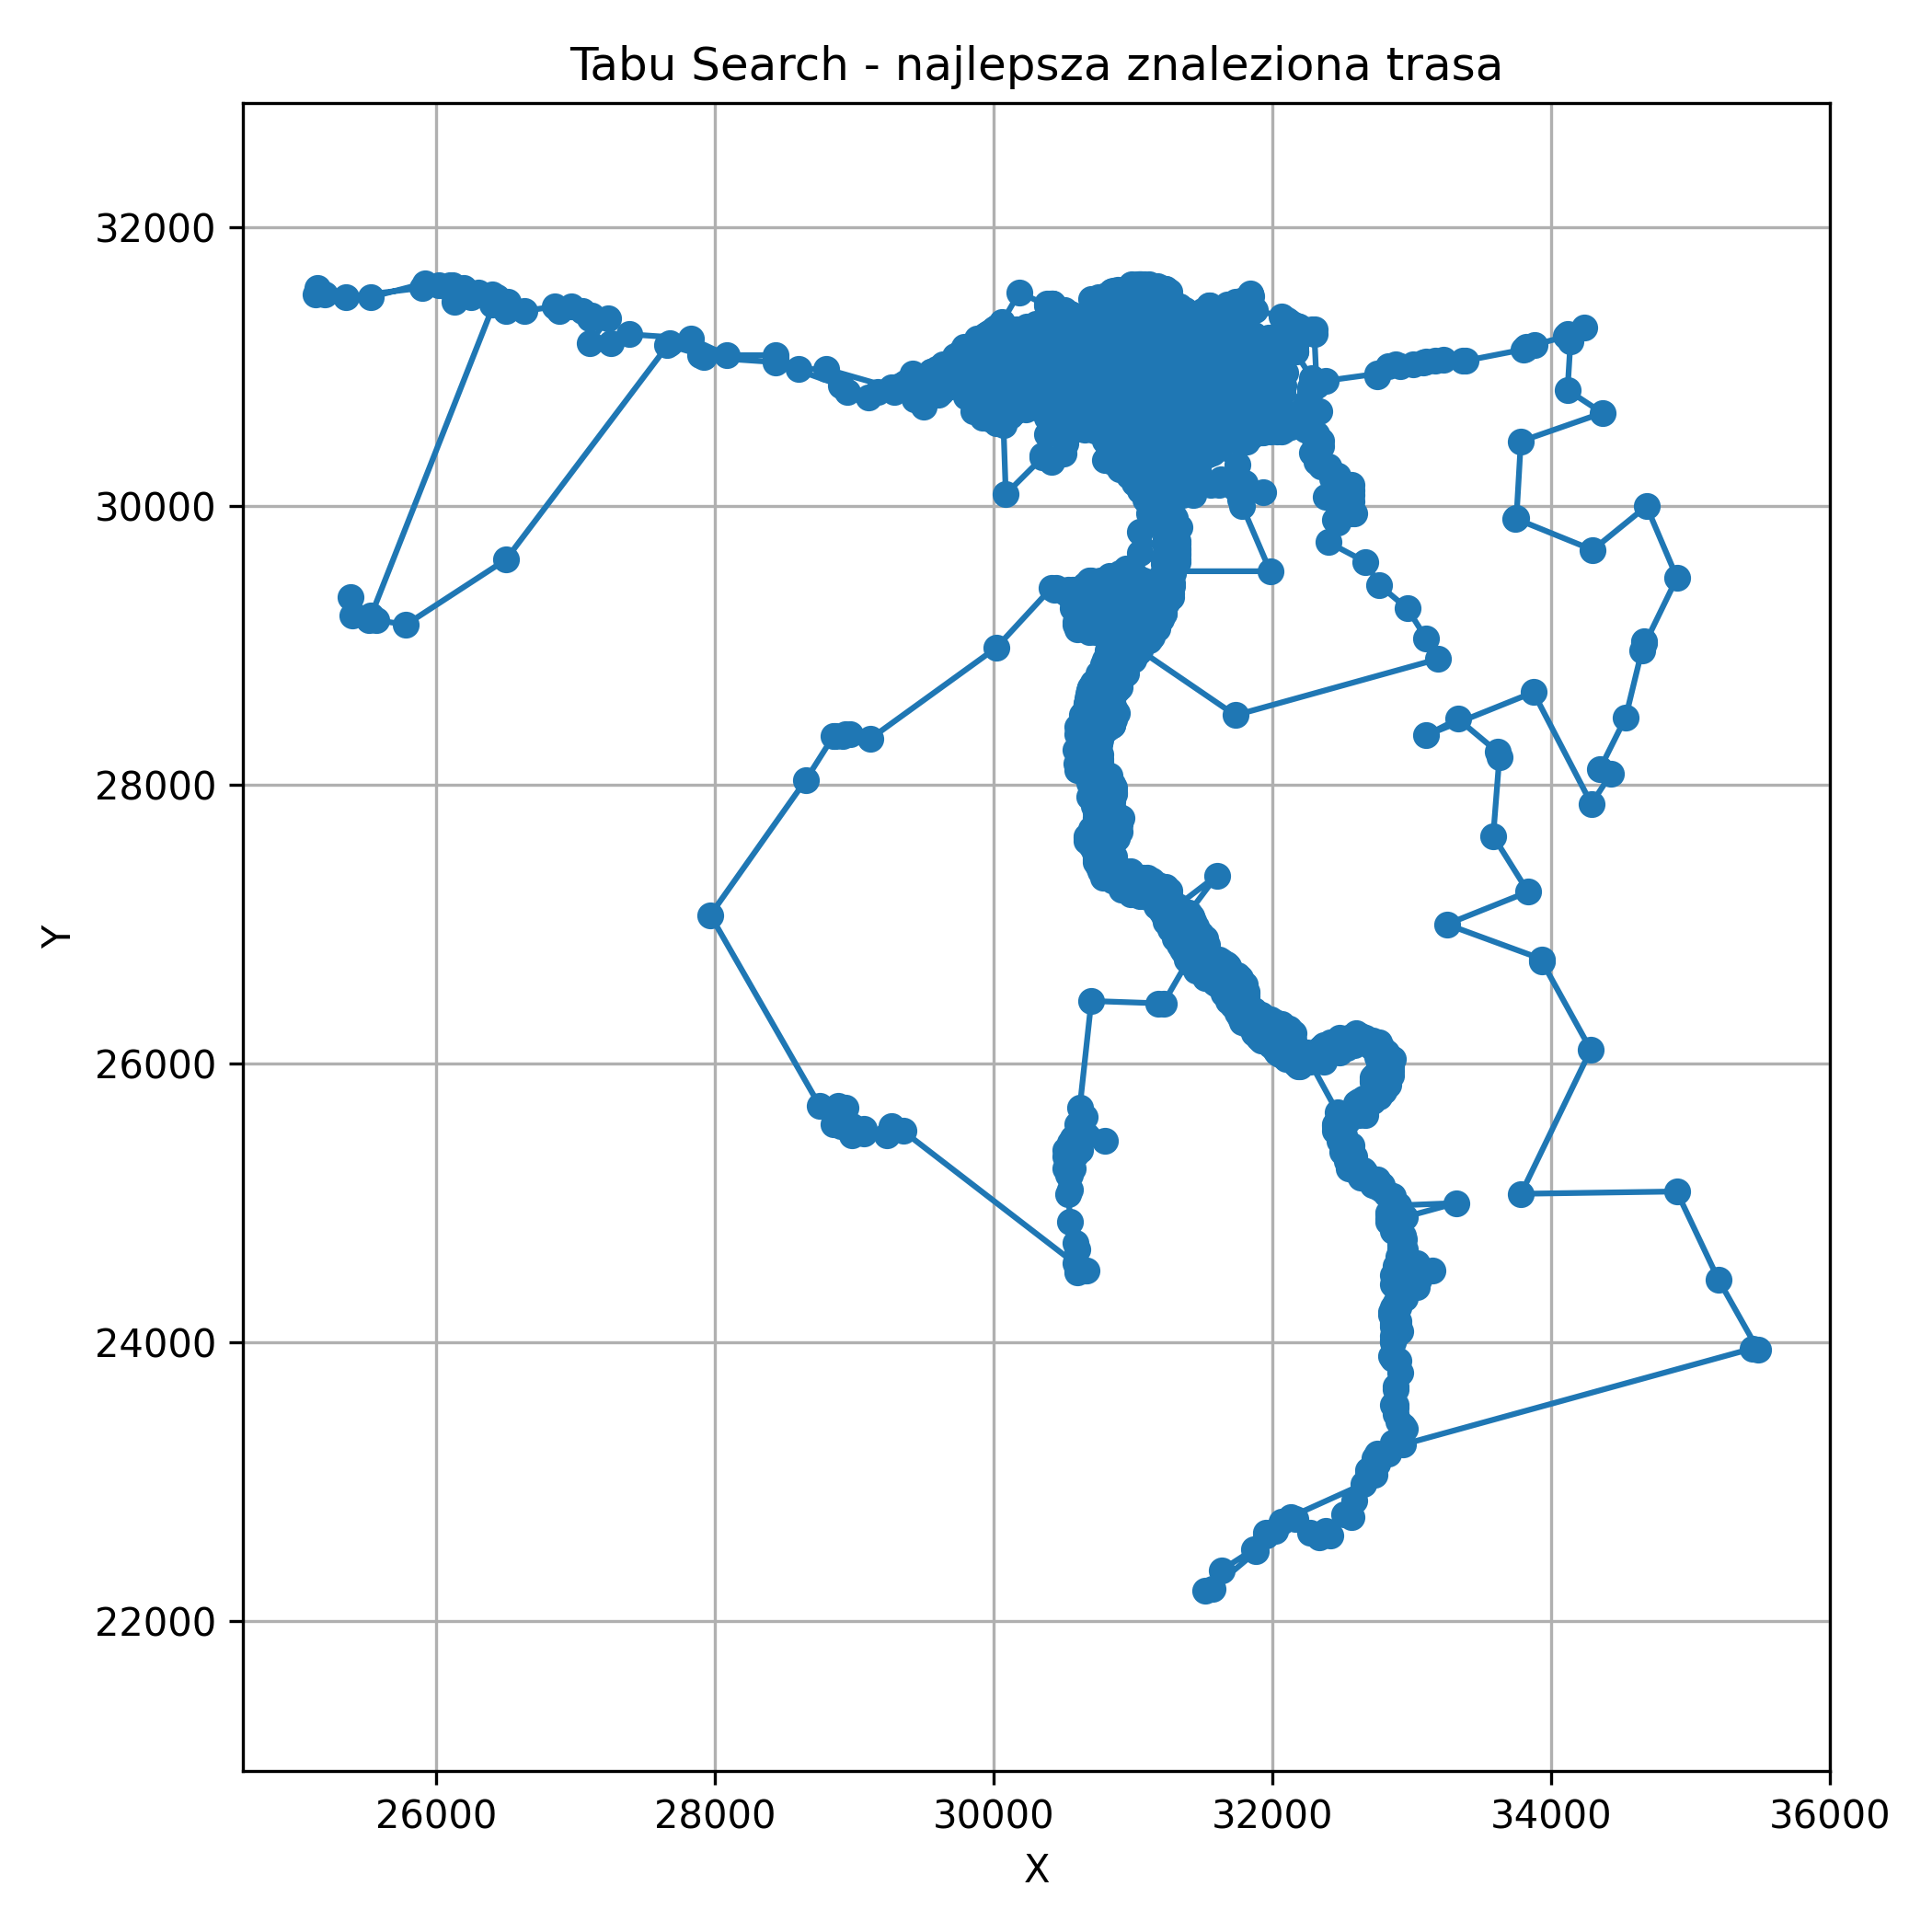
\includegraphics[width=0.8\textwidth]{tabu/tabu_best_route_eg7146.png}
    \caption{Najlepsza trasa znaleziona przez Tabu Search dla instancji \texttt{eg7146.tsp}.}
\end{figure}

\subsubsection{Instancja \texttt{ar9152.tsp}}

\begin{figure}[H]
    \centering
    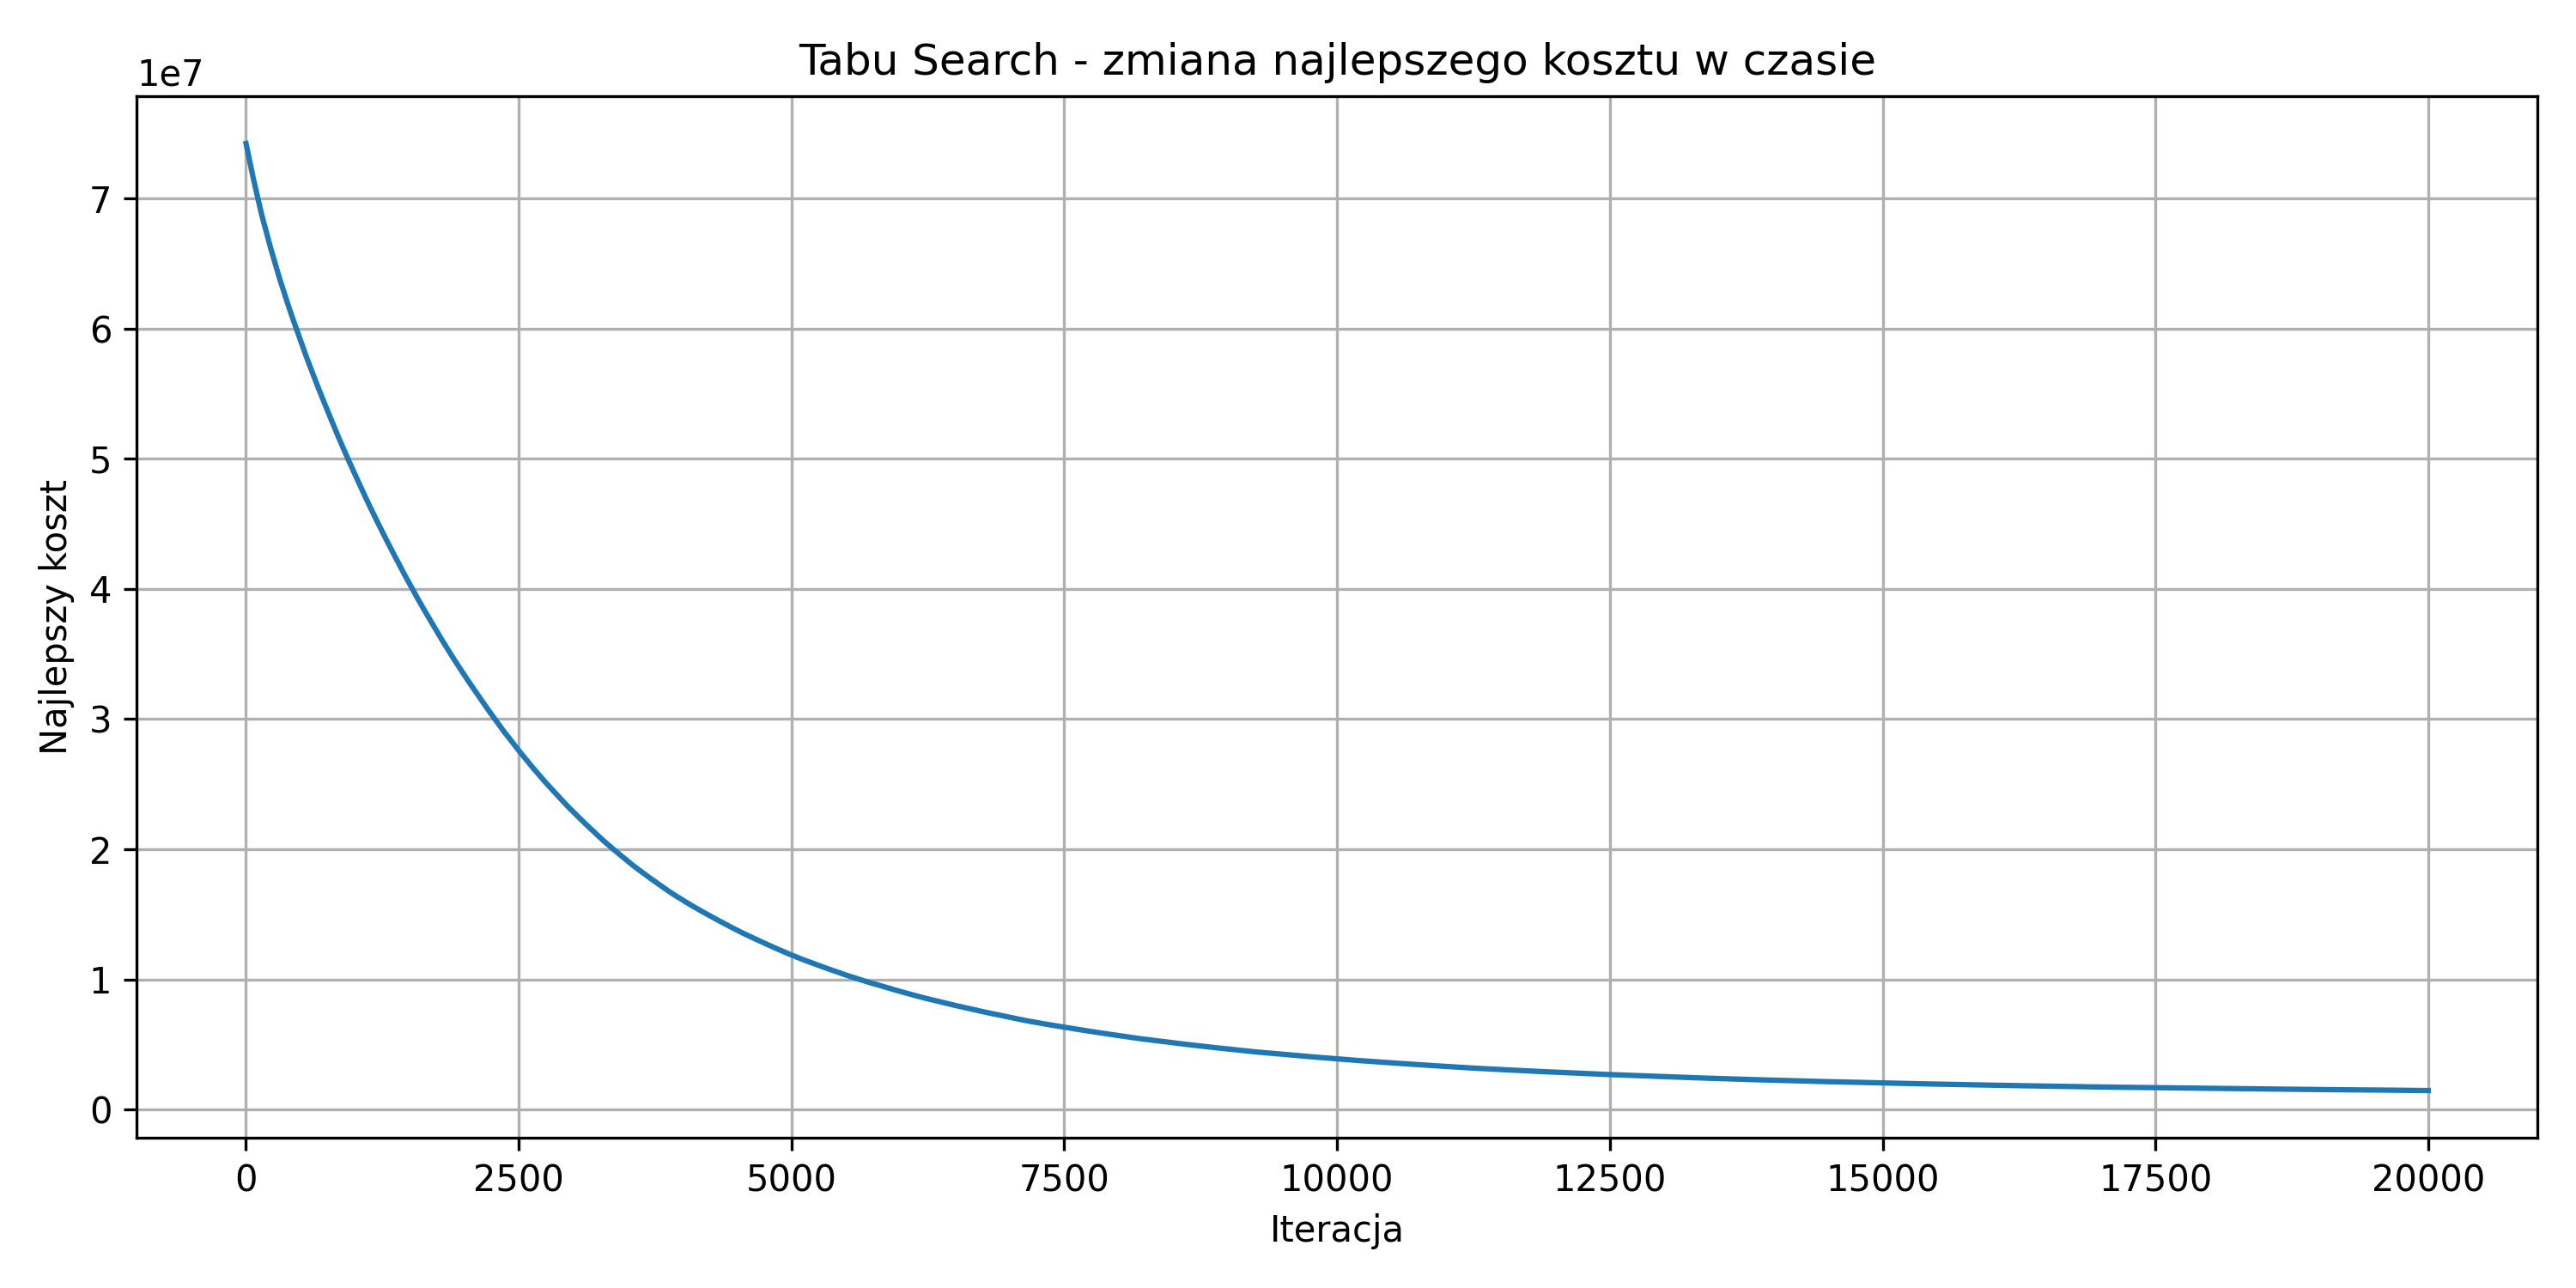
\includegraphics[width=0.9\textwidth]{tabu/tabu_history_ar9152.png}
    \caption{Zmiana najlepszego kosztu w kolejnych iteracjach Tabu Search dla instancji \texttt{ar9152.tsp}.}
\end{figure}

\begin{figure}[H]
    \centering
    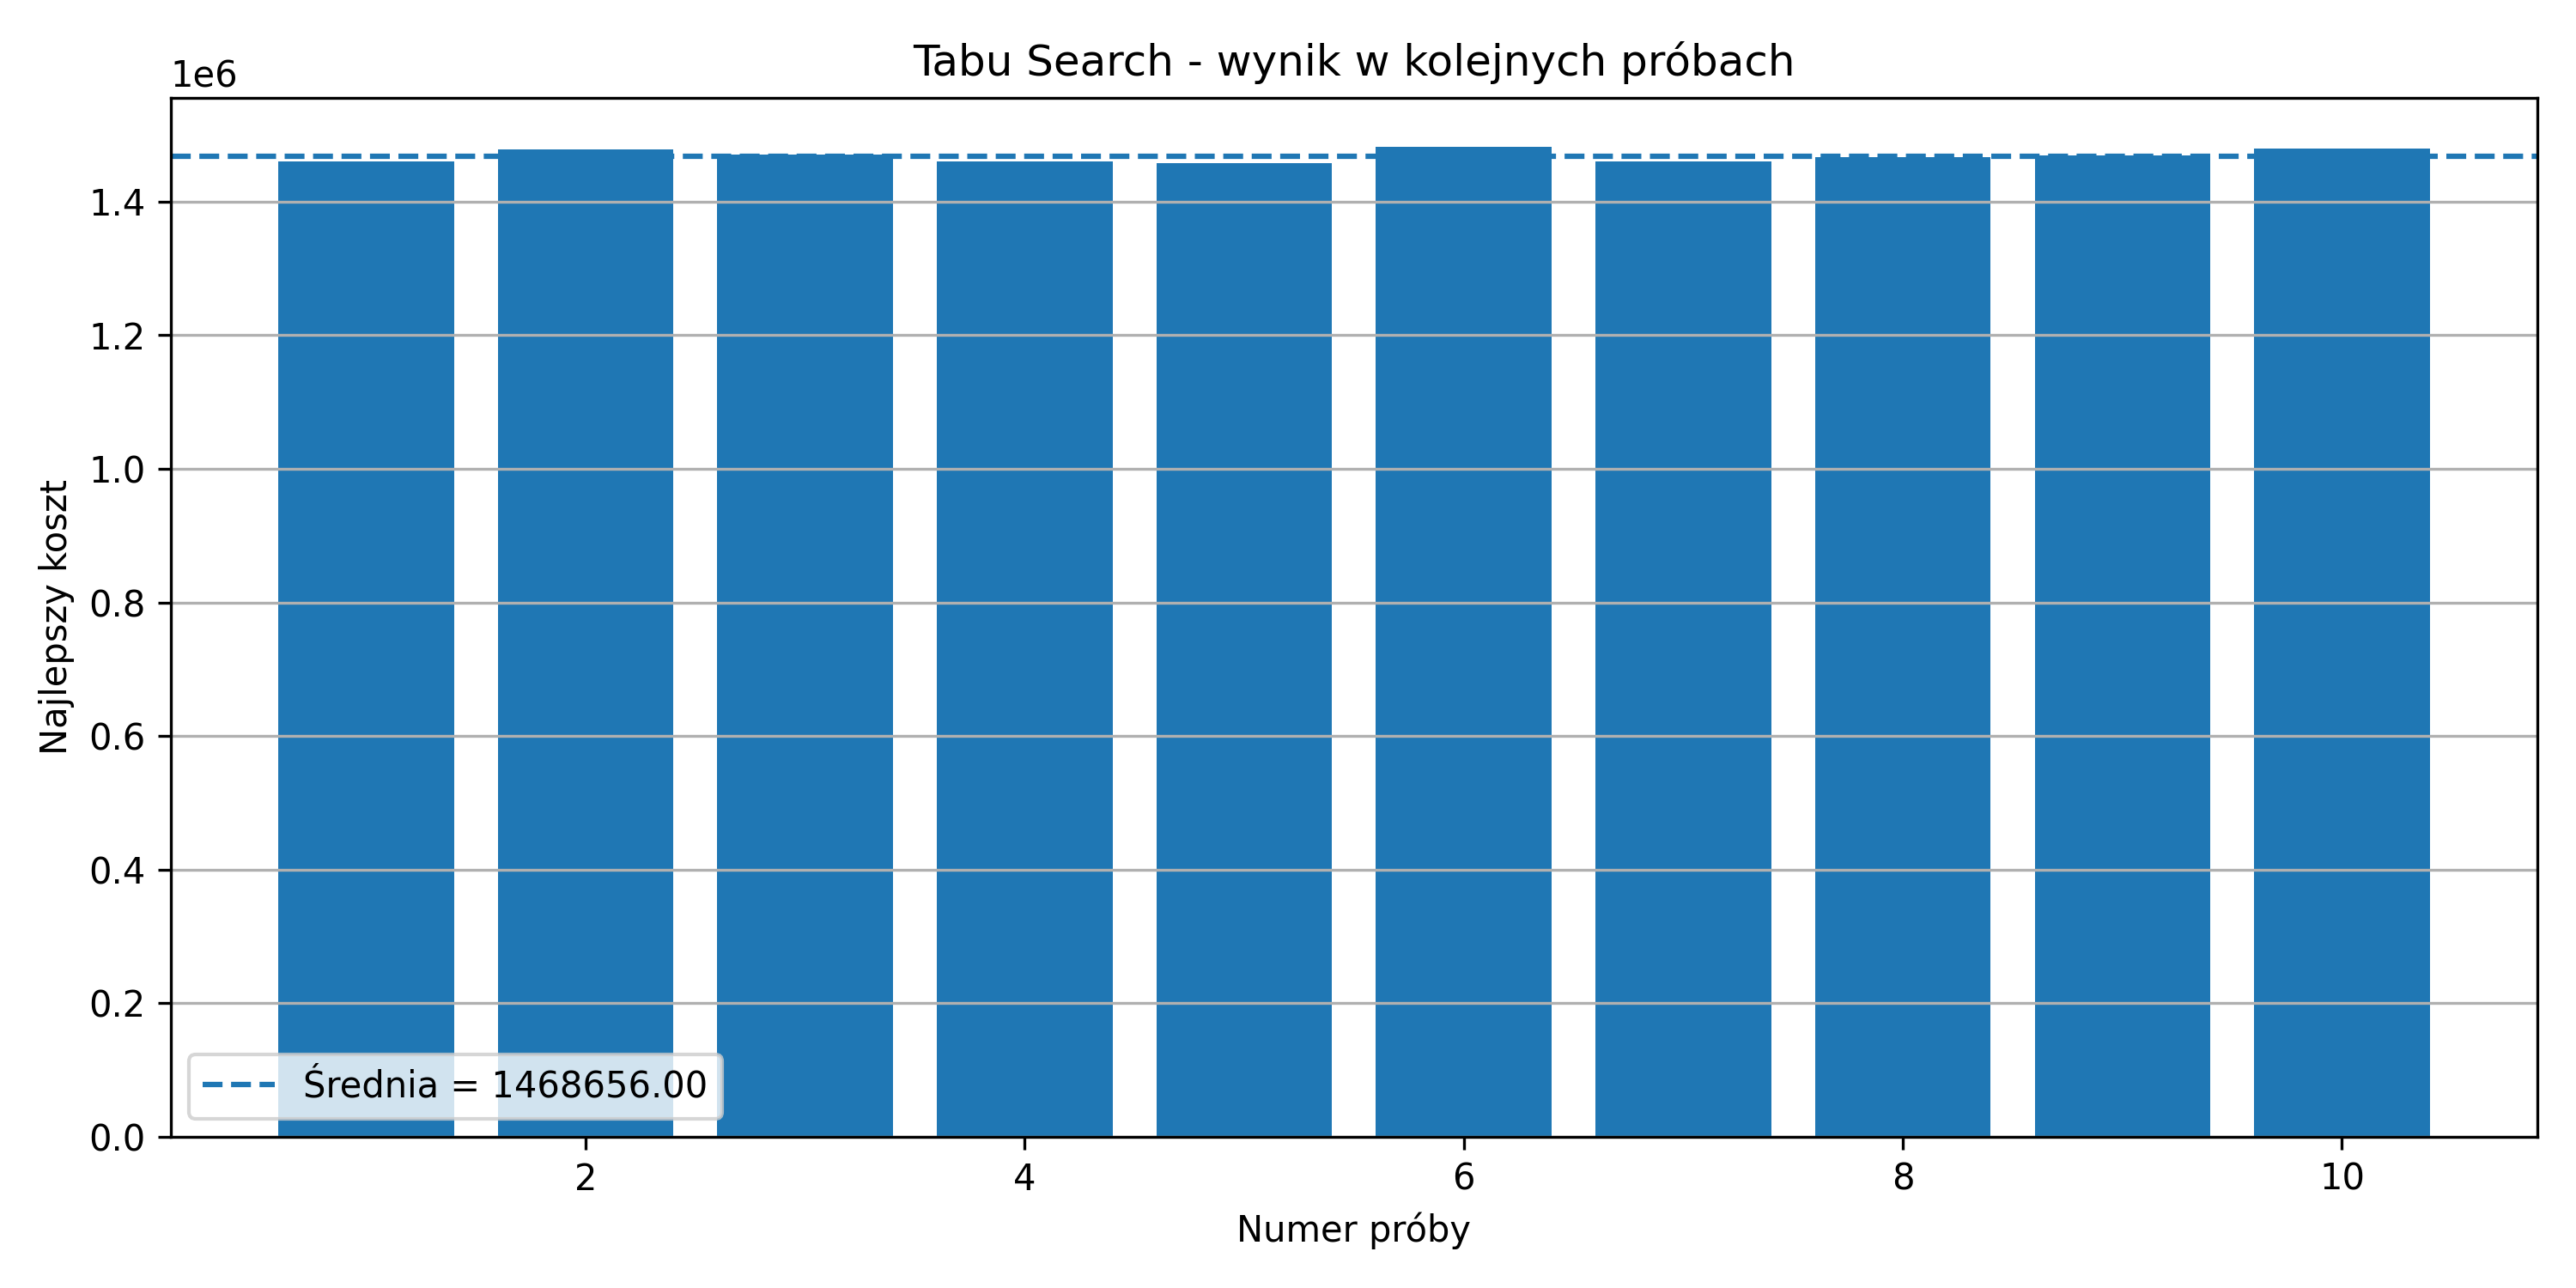
\includegraphics[width=0.9\textwidth]{tabu/tabu_runs_bar_ar9152.png}
    \caption{Najlepsze wyniki uzyskane w kolejnych próbach Tabu Search dla instancji \texttt{ar9152.tsp}.}
\end{figure}

\begin{figure}[H]
    \centering
    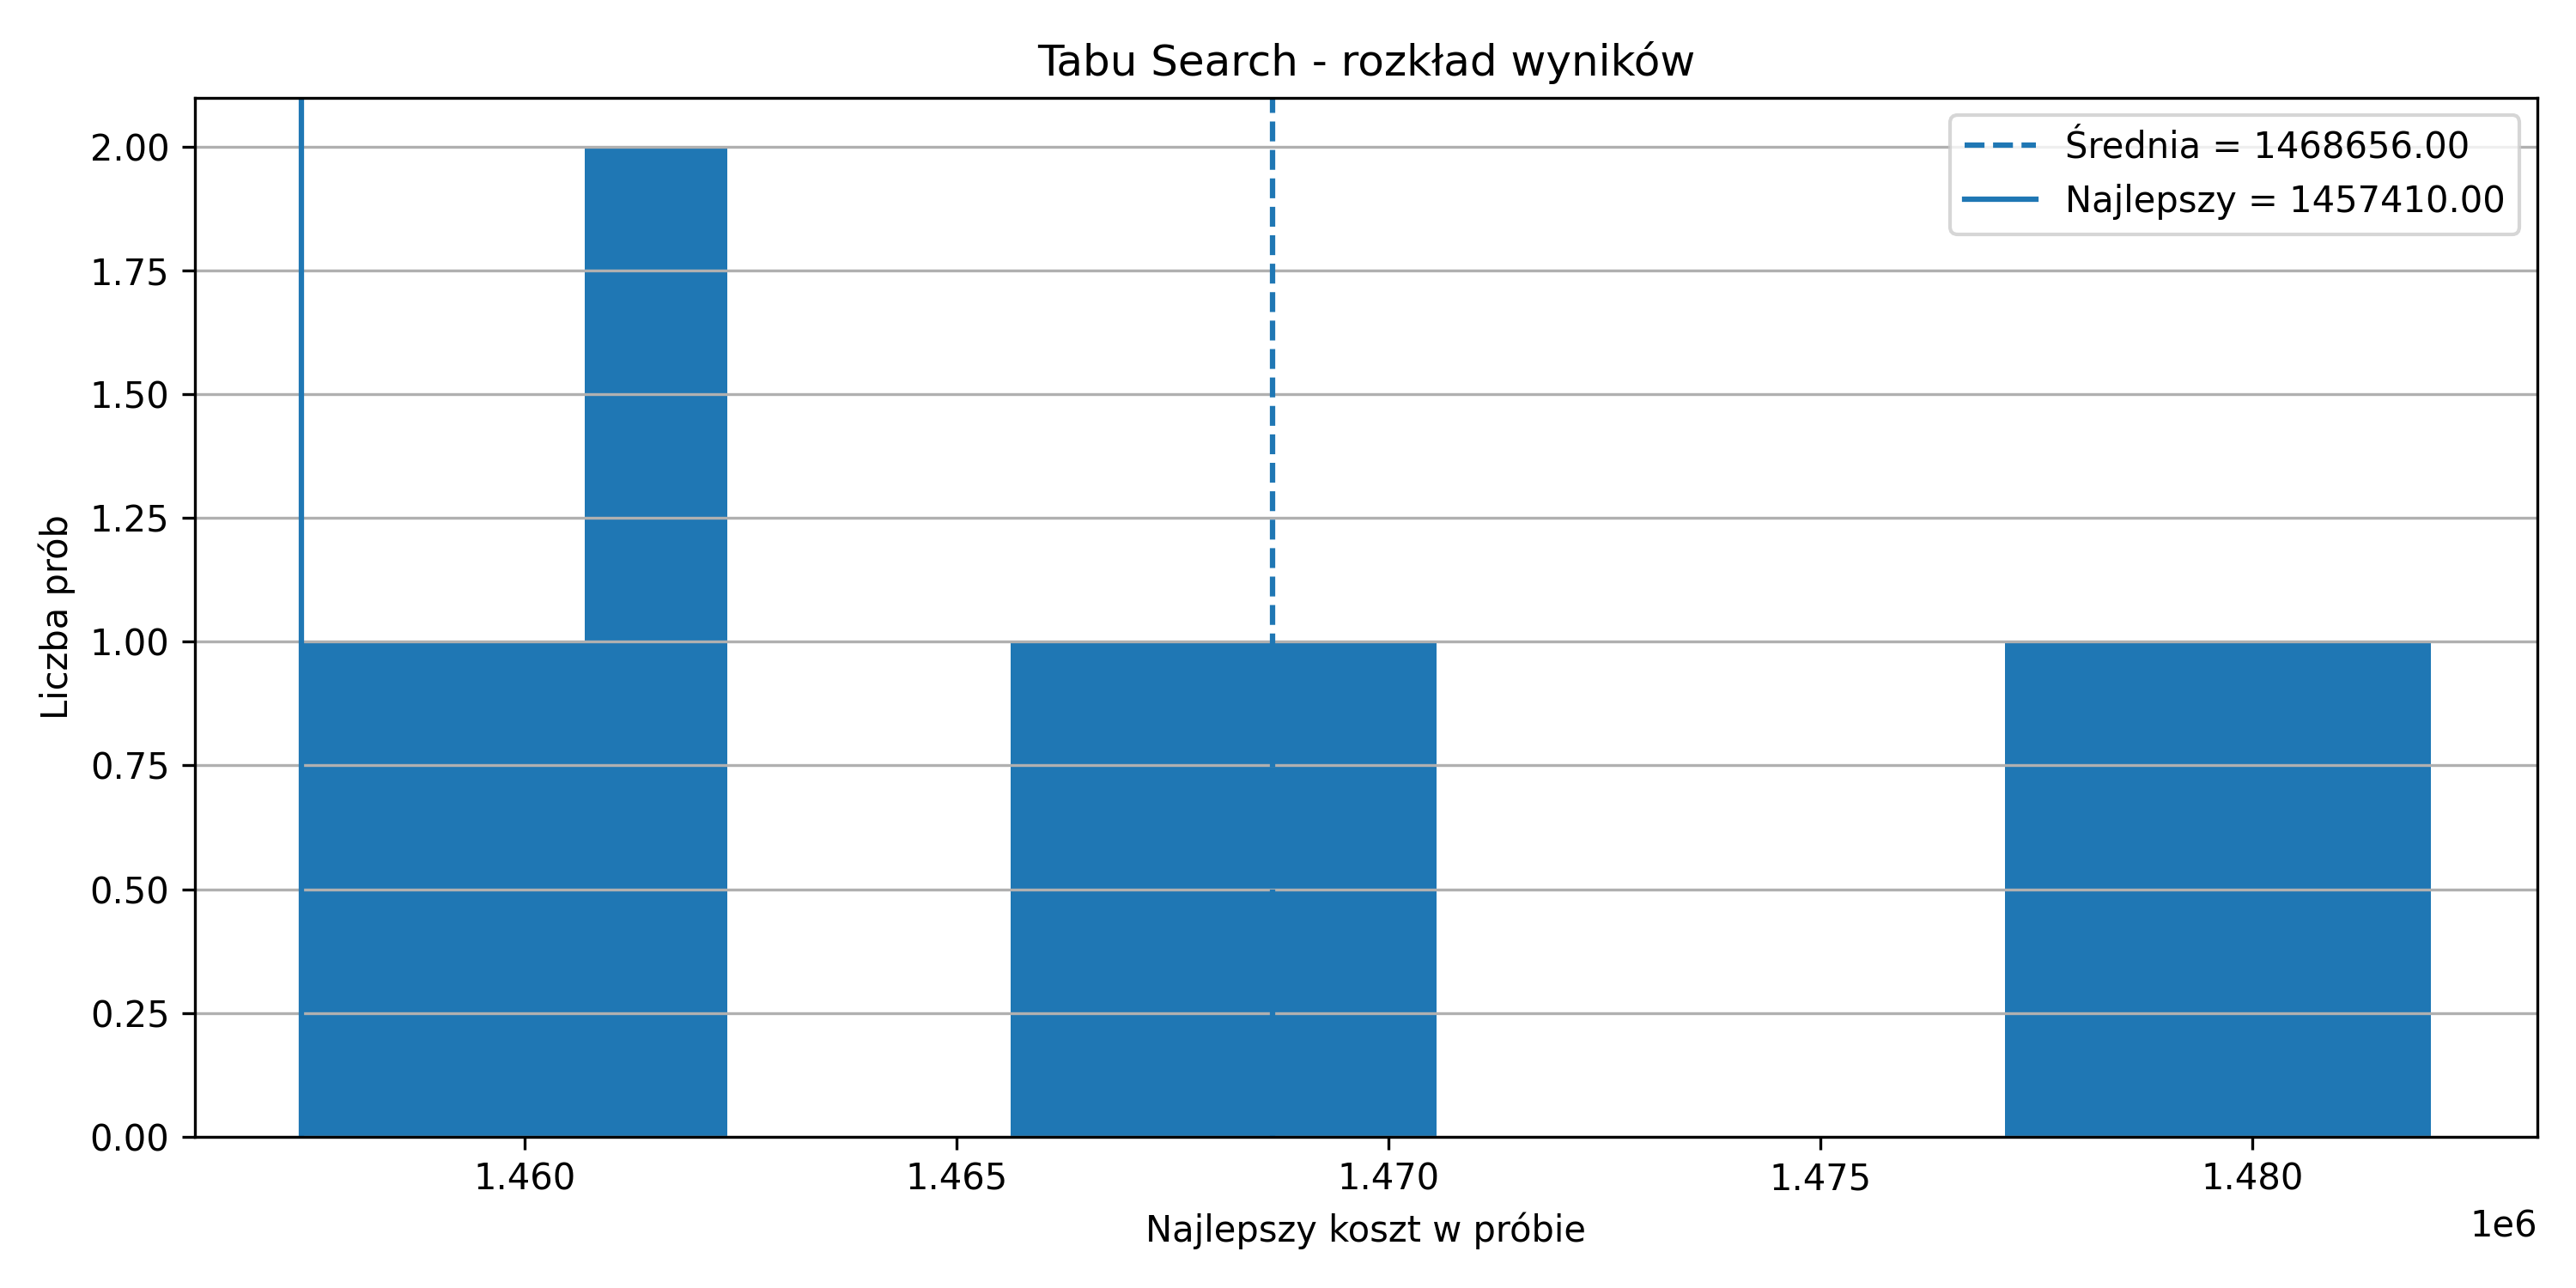
\includegraphics[width=0.9\textwidth]{tabu/tabu_runs_histogram_ar9152.png}
    \caption{Rozkład wyników uzyskanych w próbach Tabu Search dla instancji \texttt{ar9152.tsp}.}
\end{figure}

\begin{figure}[H]
    \centering
    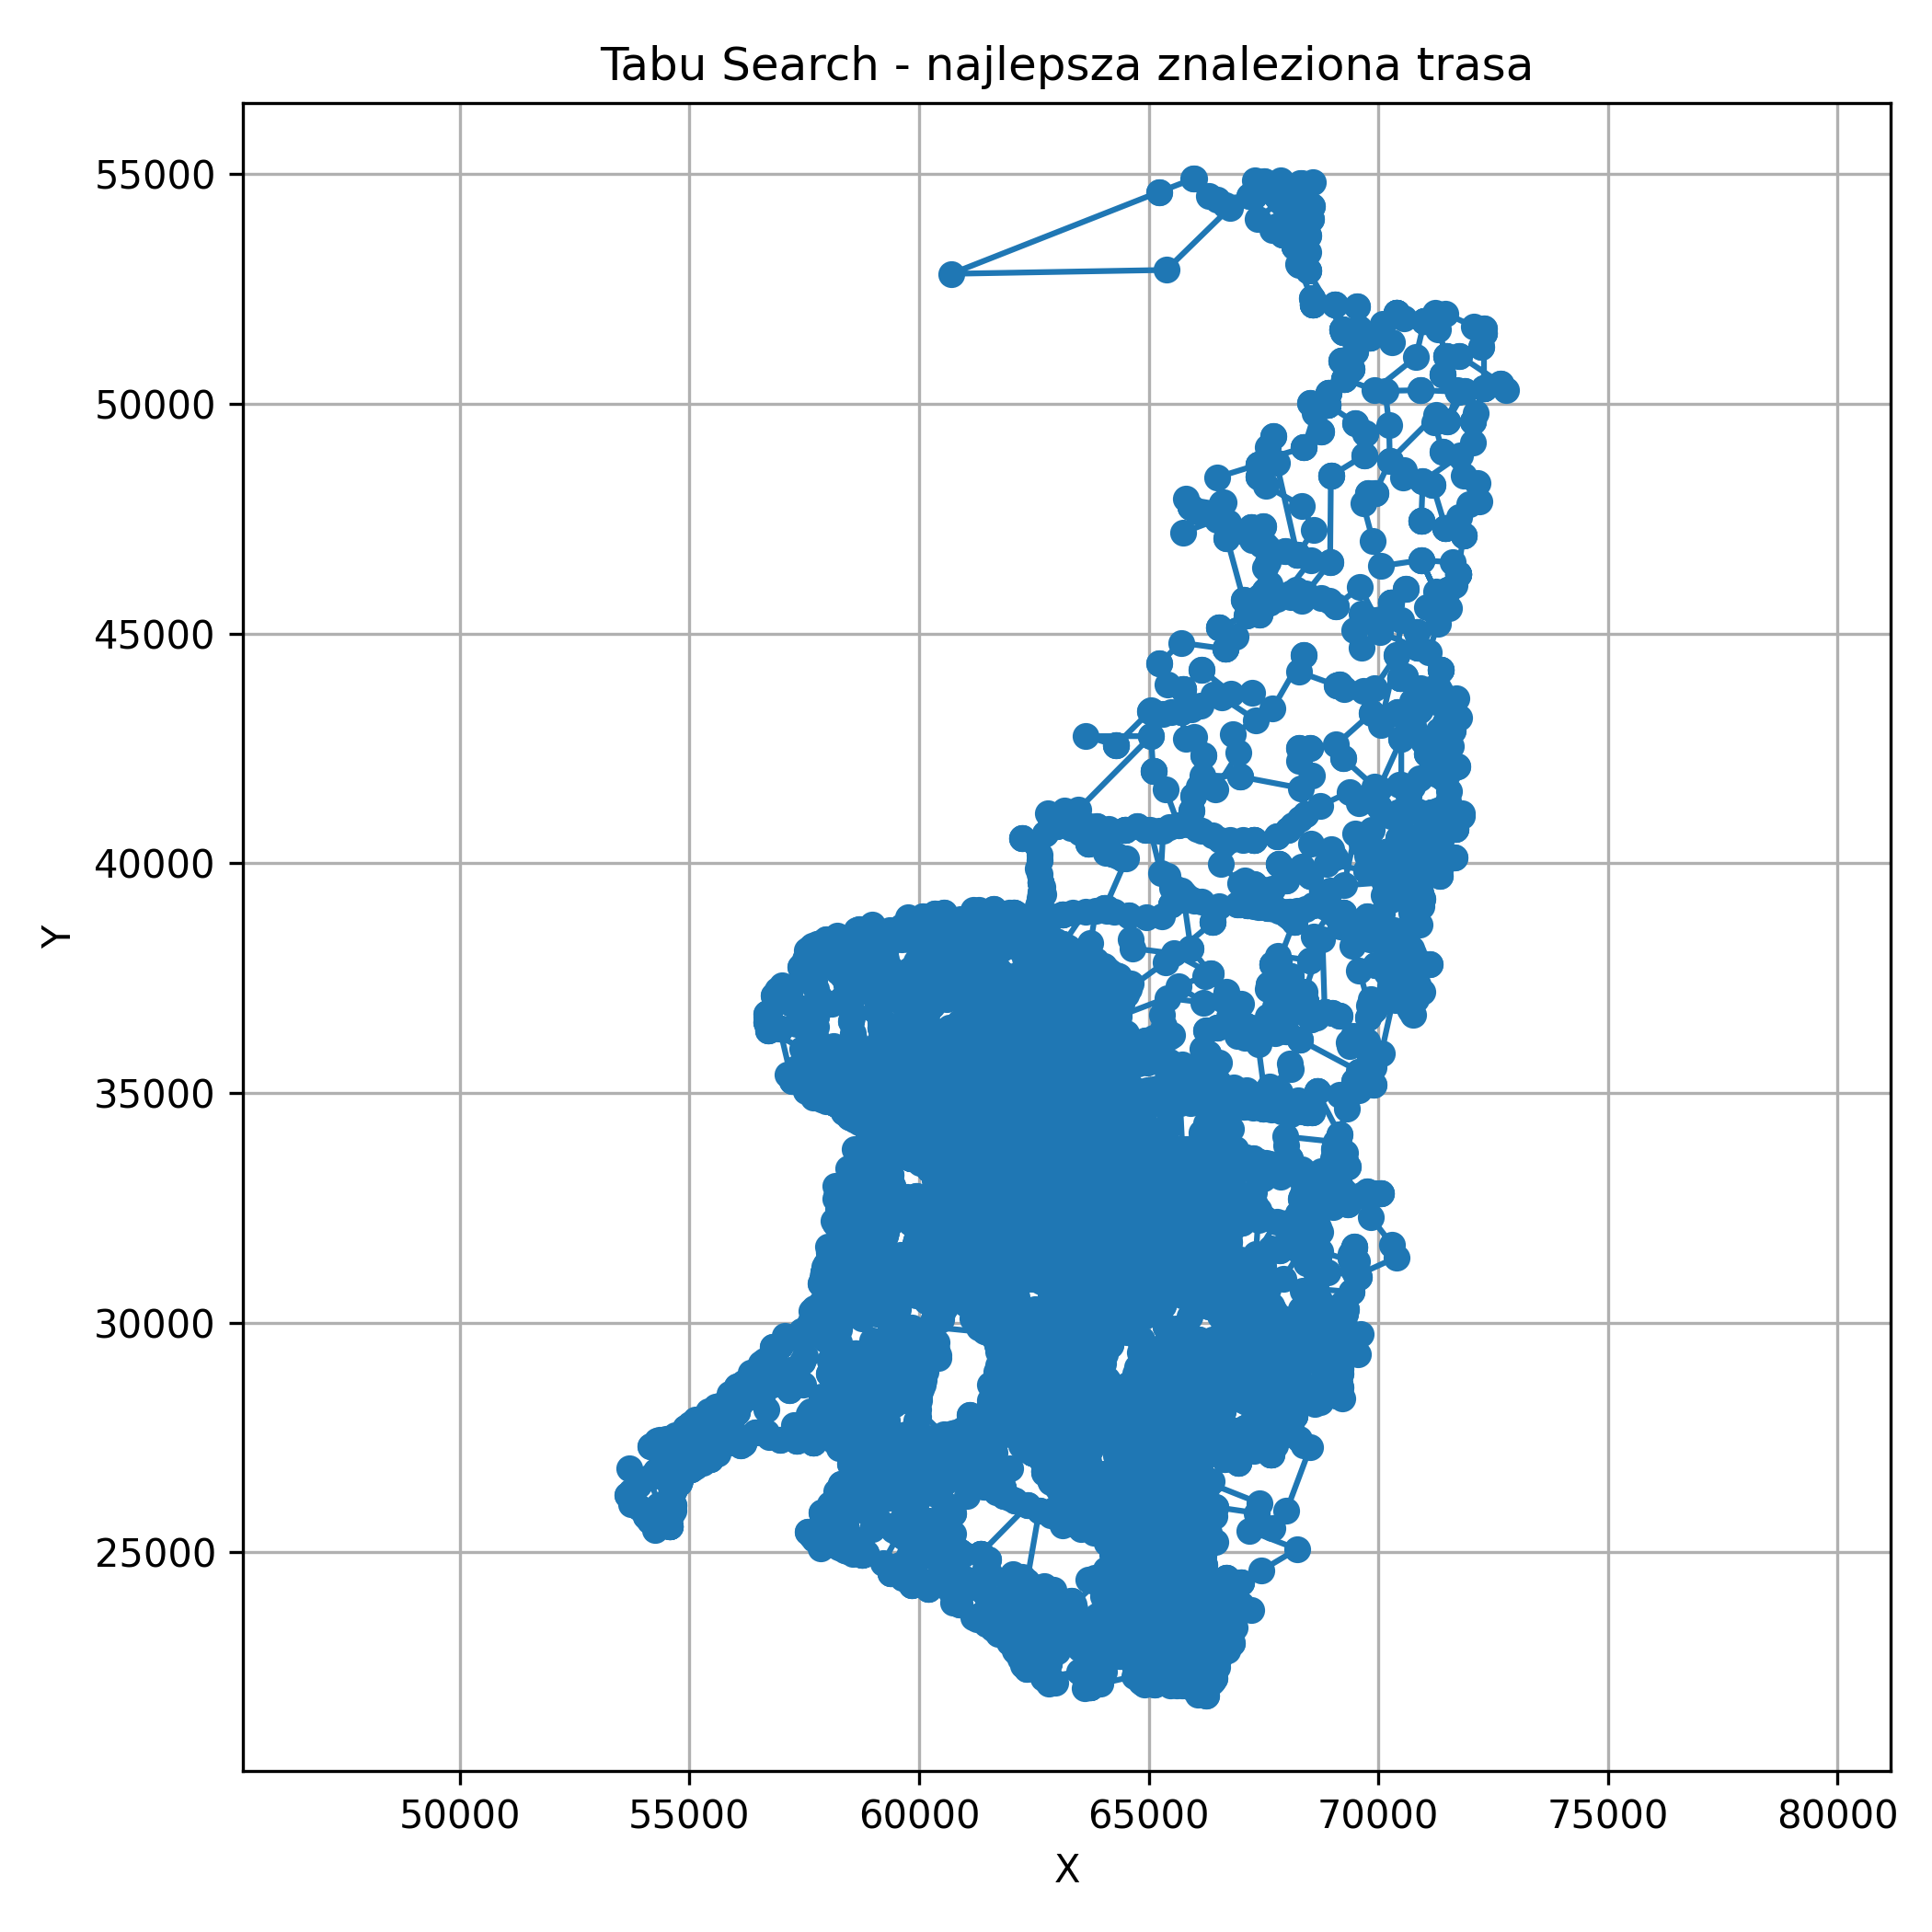
\includegraphics[width=0.8\textwidth]{tabu/tabu_best_route_ar9152.png}
    \caption{Najlepsza trasa znaleziona przez Tabu Search dla instancji \texttt{ar9152.tsp}.}
\end{figure}

\subsubsection{Instancja \texttt{it16862.tsp}}

\begin{figure}[H]
    \centering
    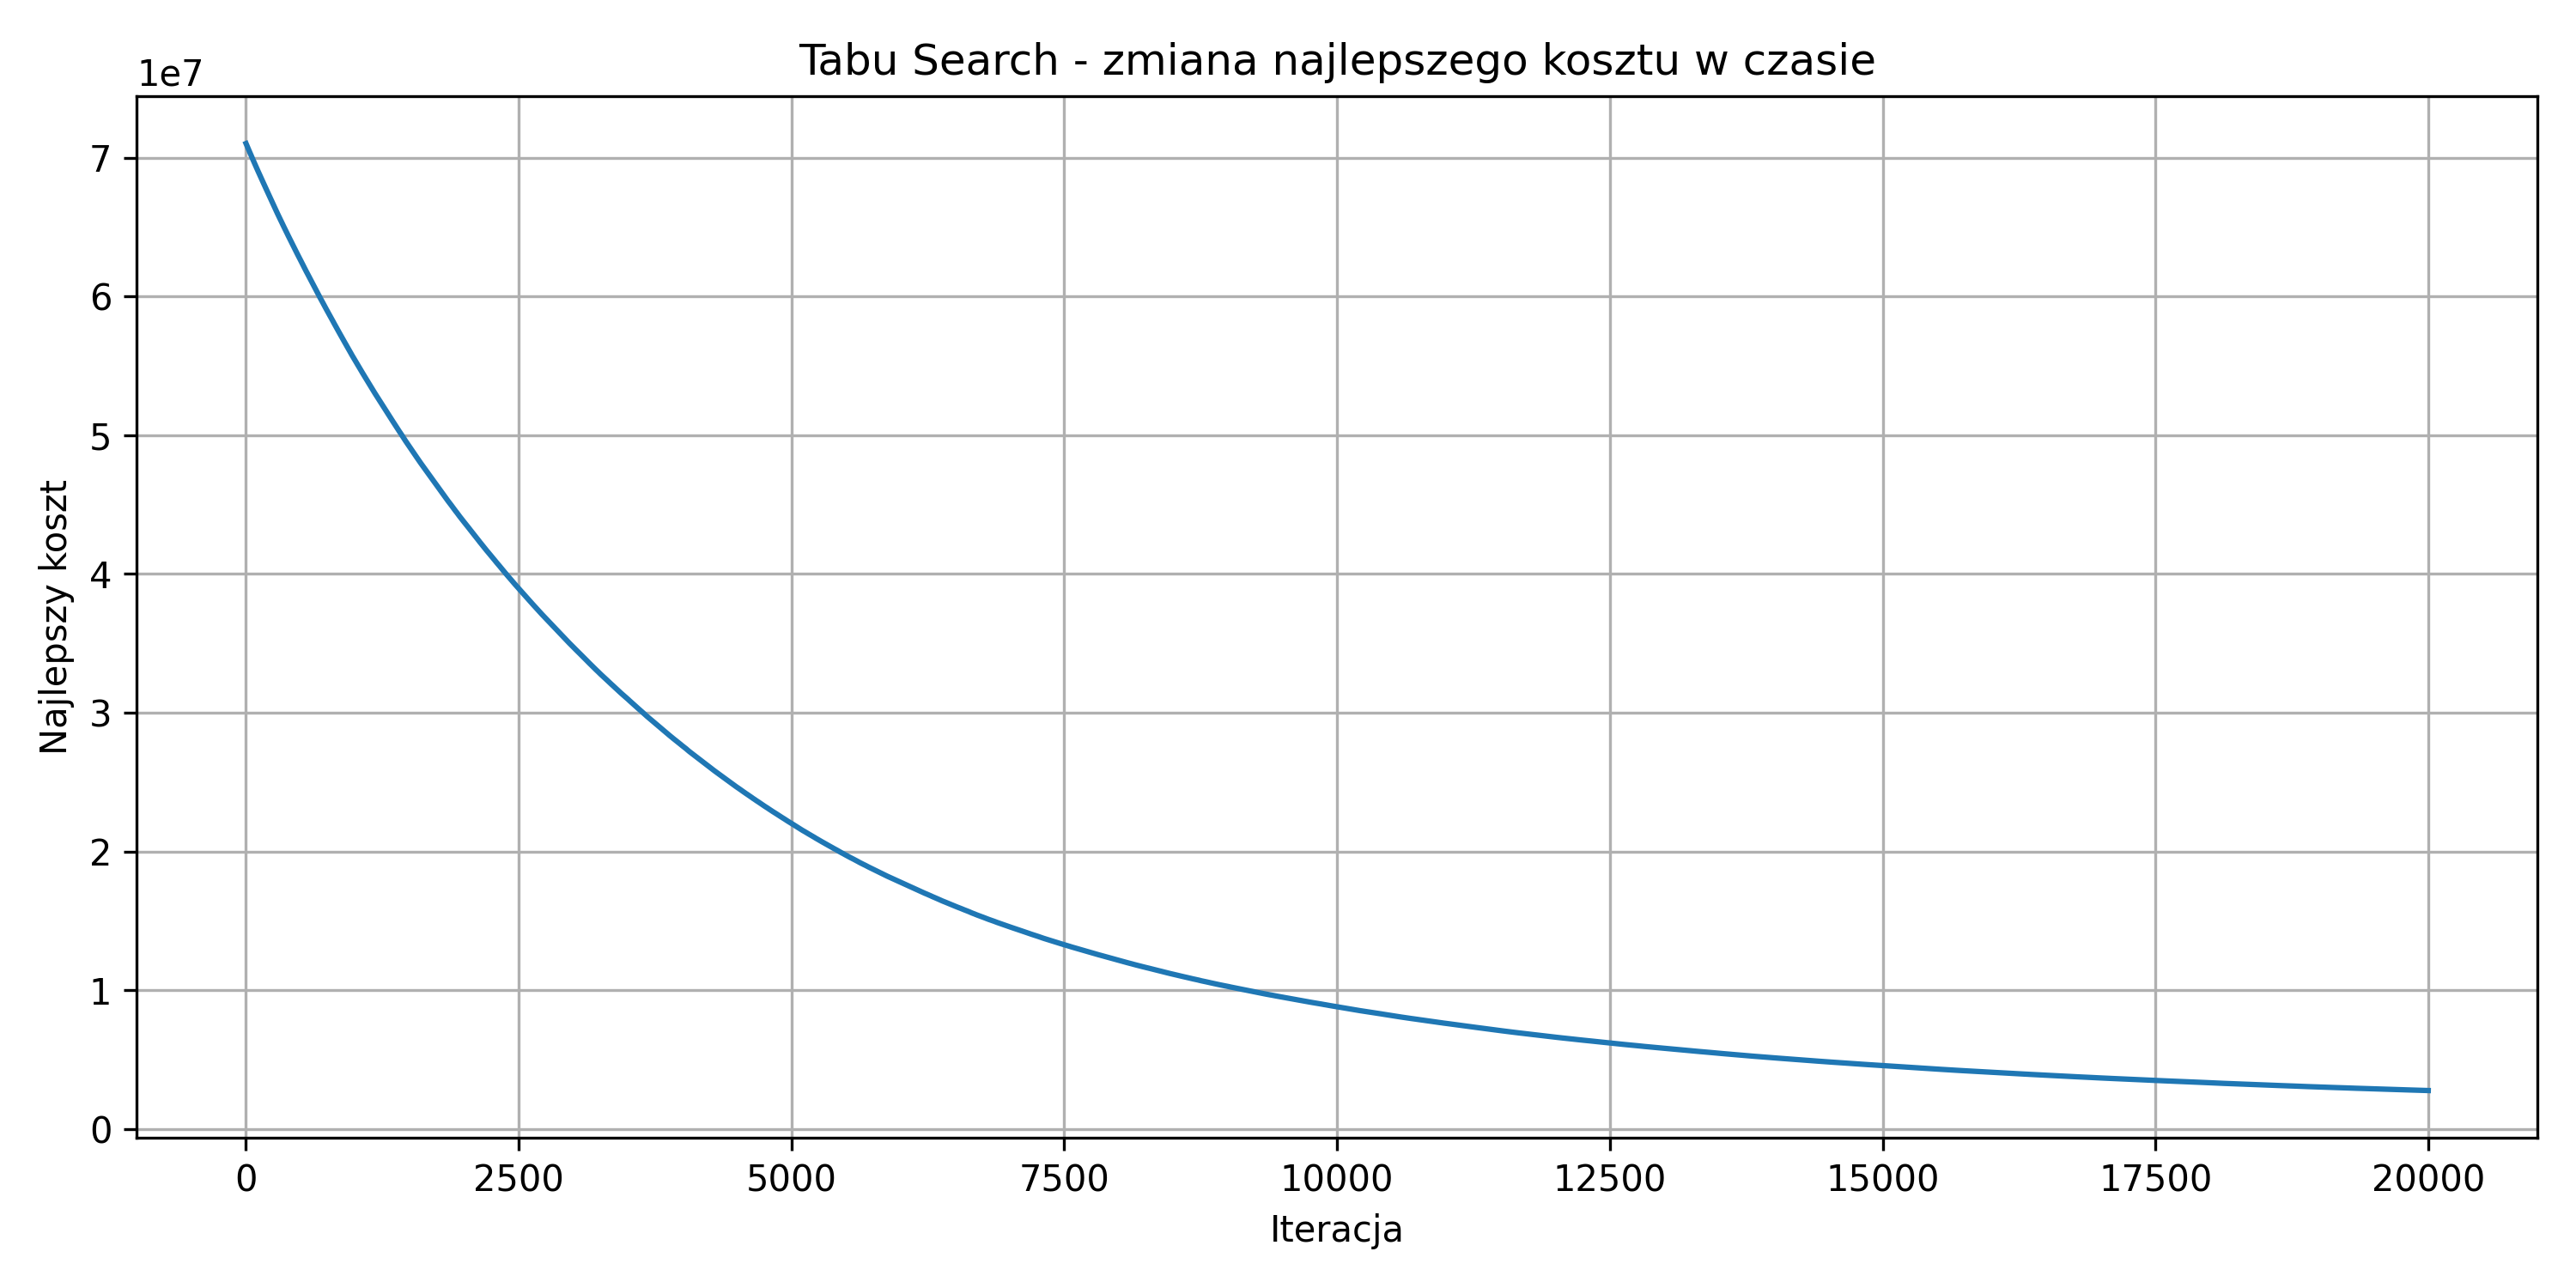
\includegraphics[width=0.9\textwidth]{tabu/tabu_history_it16862.png}
    \caption{Zmiana najlepszego kosztu w kolejnych iteracjach Tabu Search dla instancji \texttt{it16862.tsp}.}
\end{figure}

\begin{figure}[H]
    \centering
    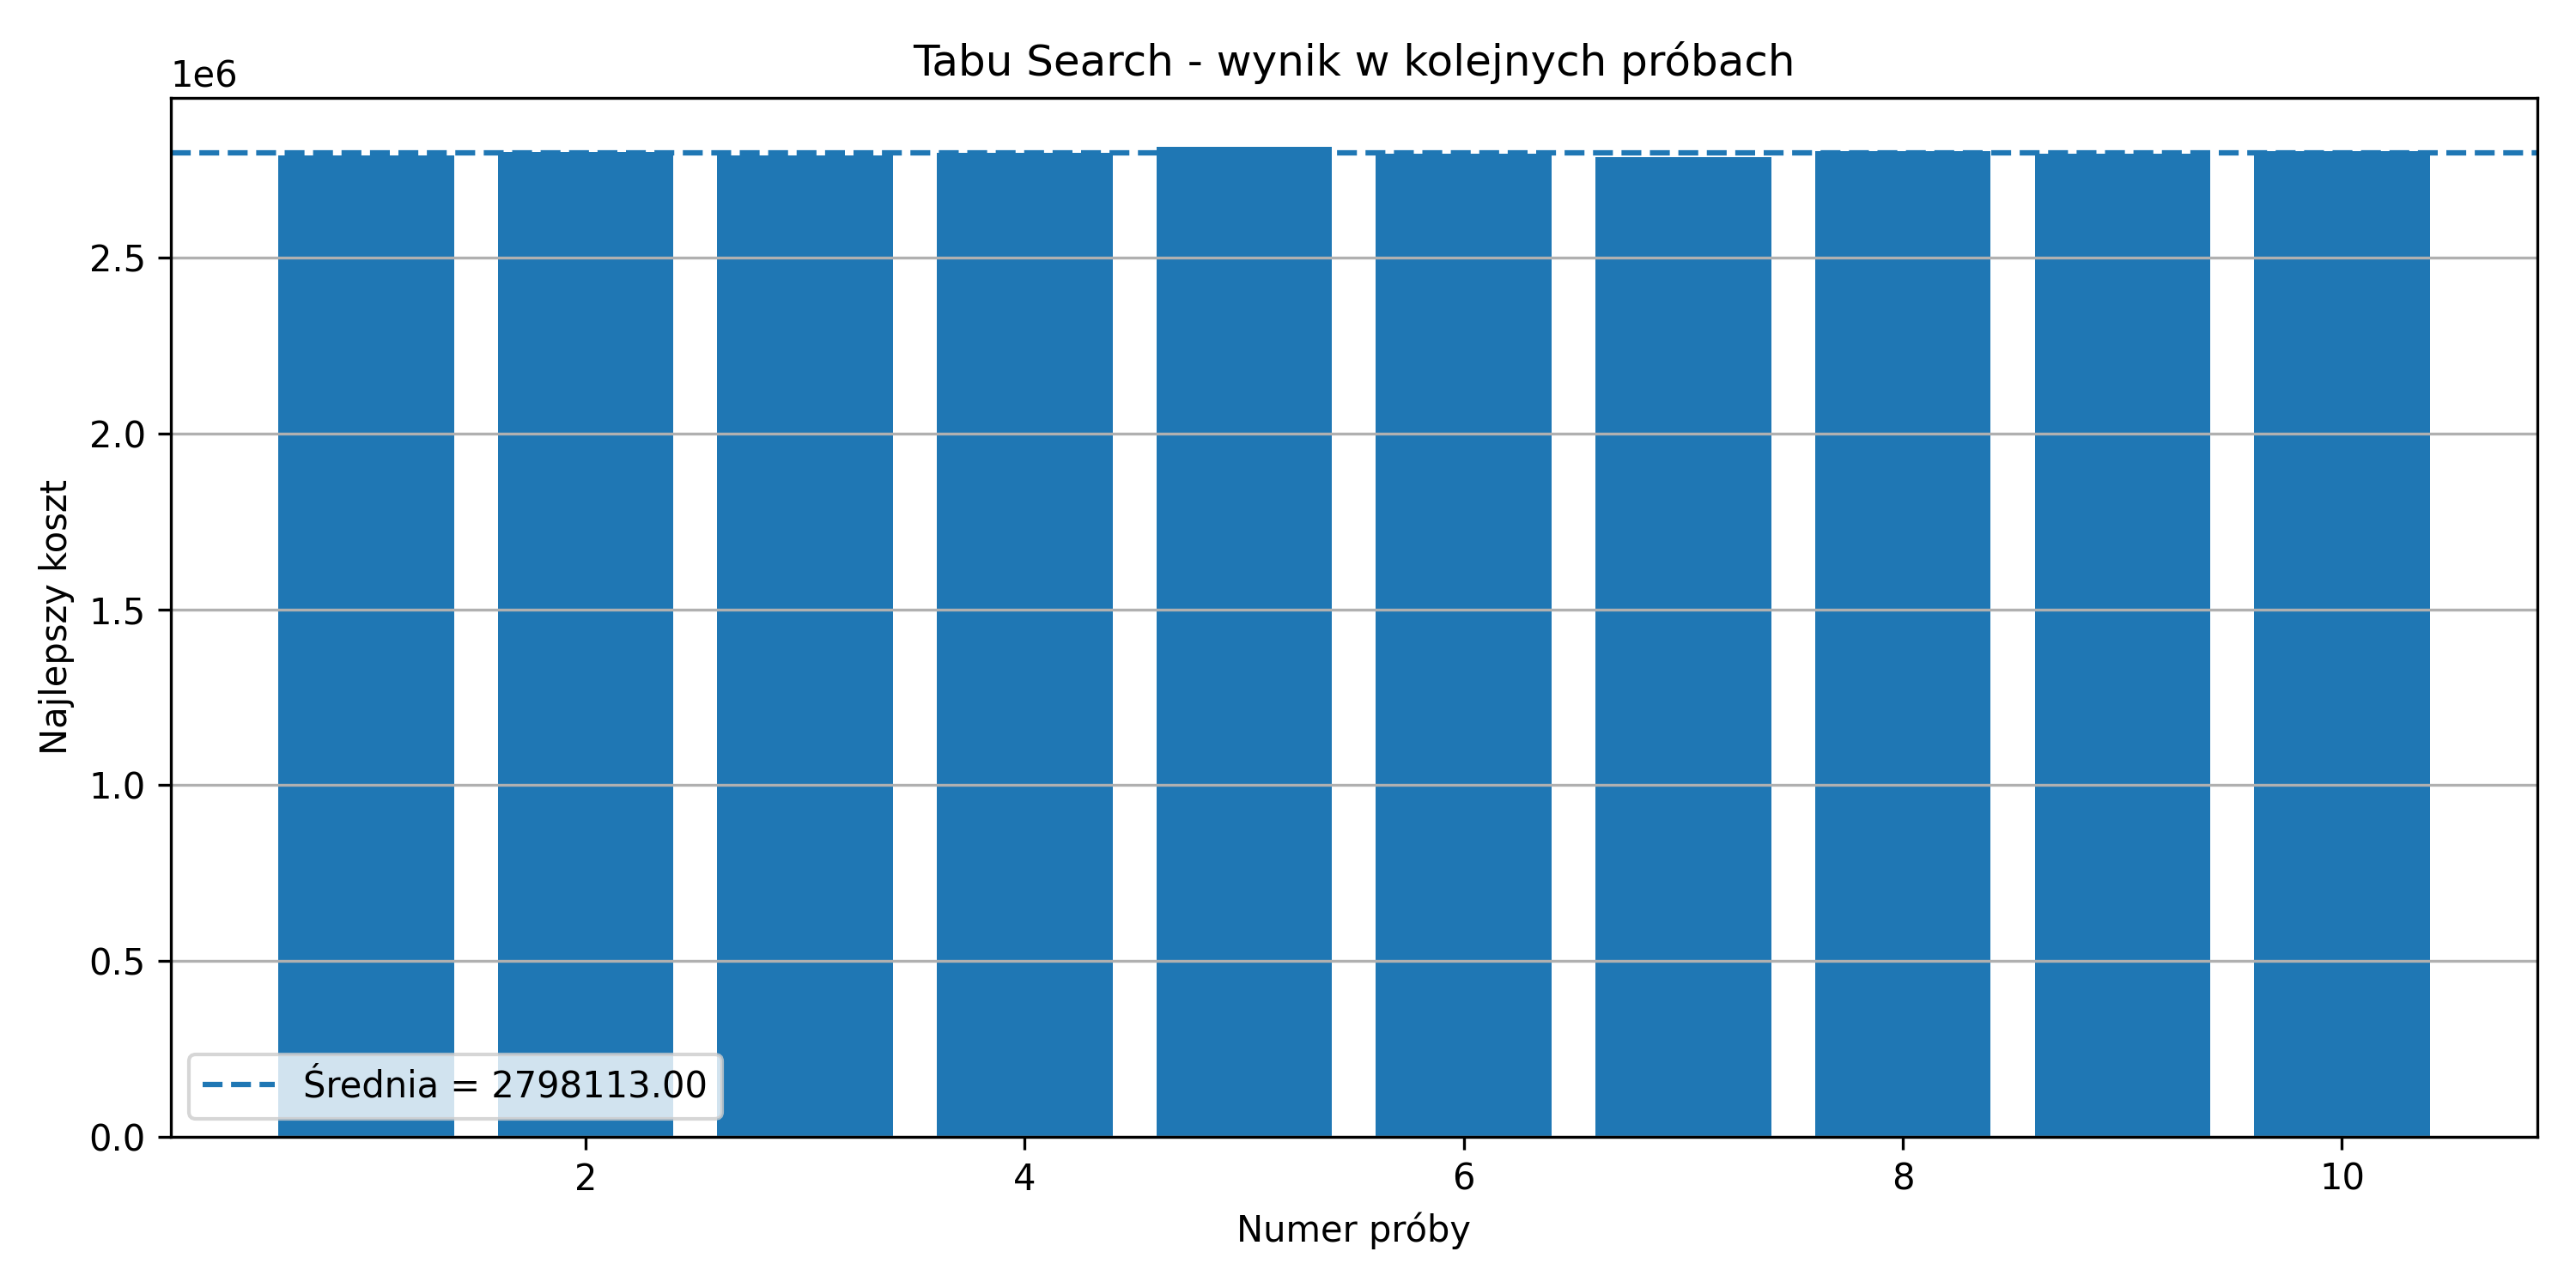
\includegraphics[width=0.9\textwidth]{tabu/tabu_runs_bar_it16862.png}
    \caption{Najlepsze wyniki uzyskane w kolejnych próbach Tabu Search dla instancji \texttt{it16862.tsp}.}
\end{figure}

\begin{figure}[H]
    \centering
    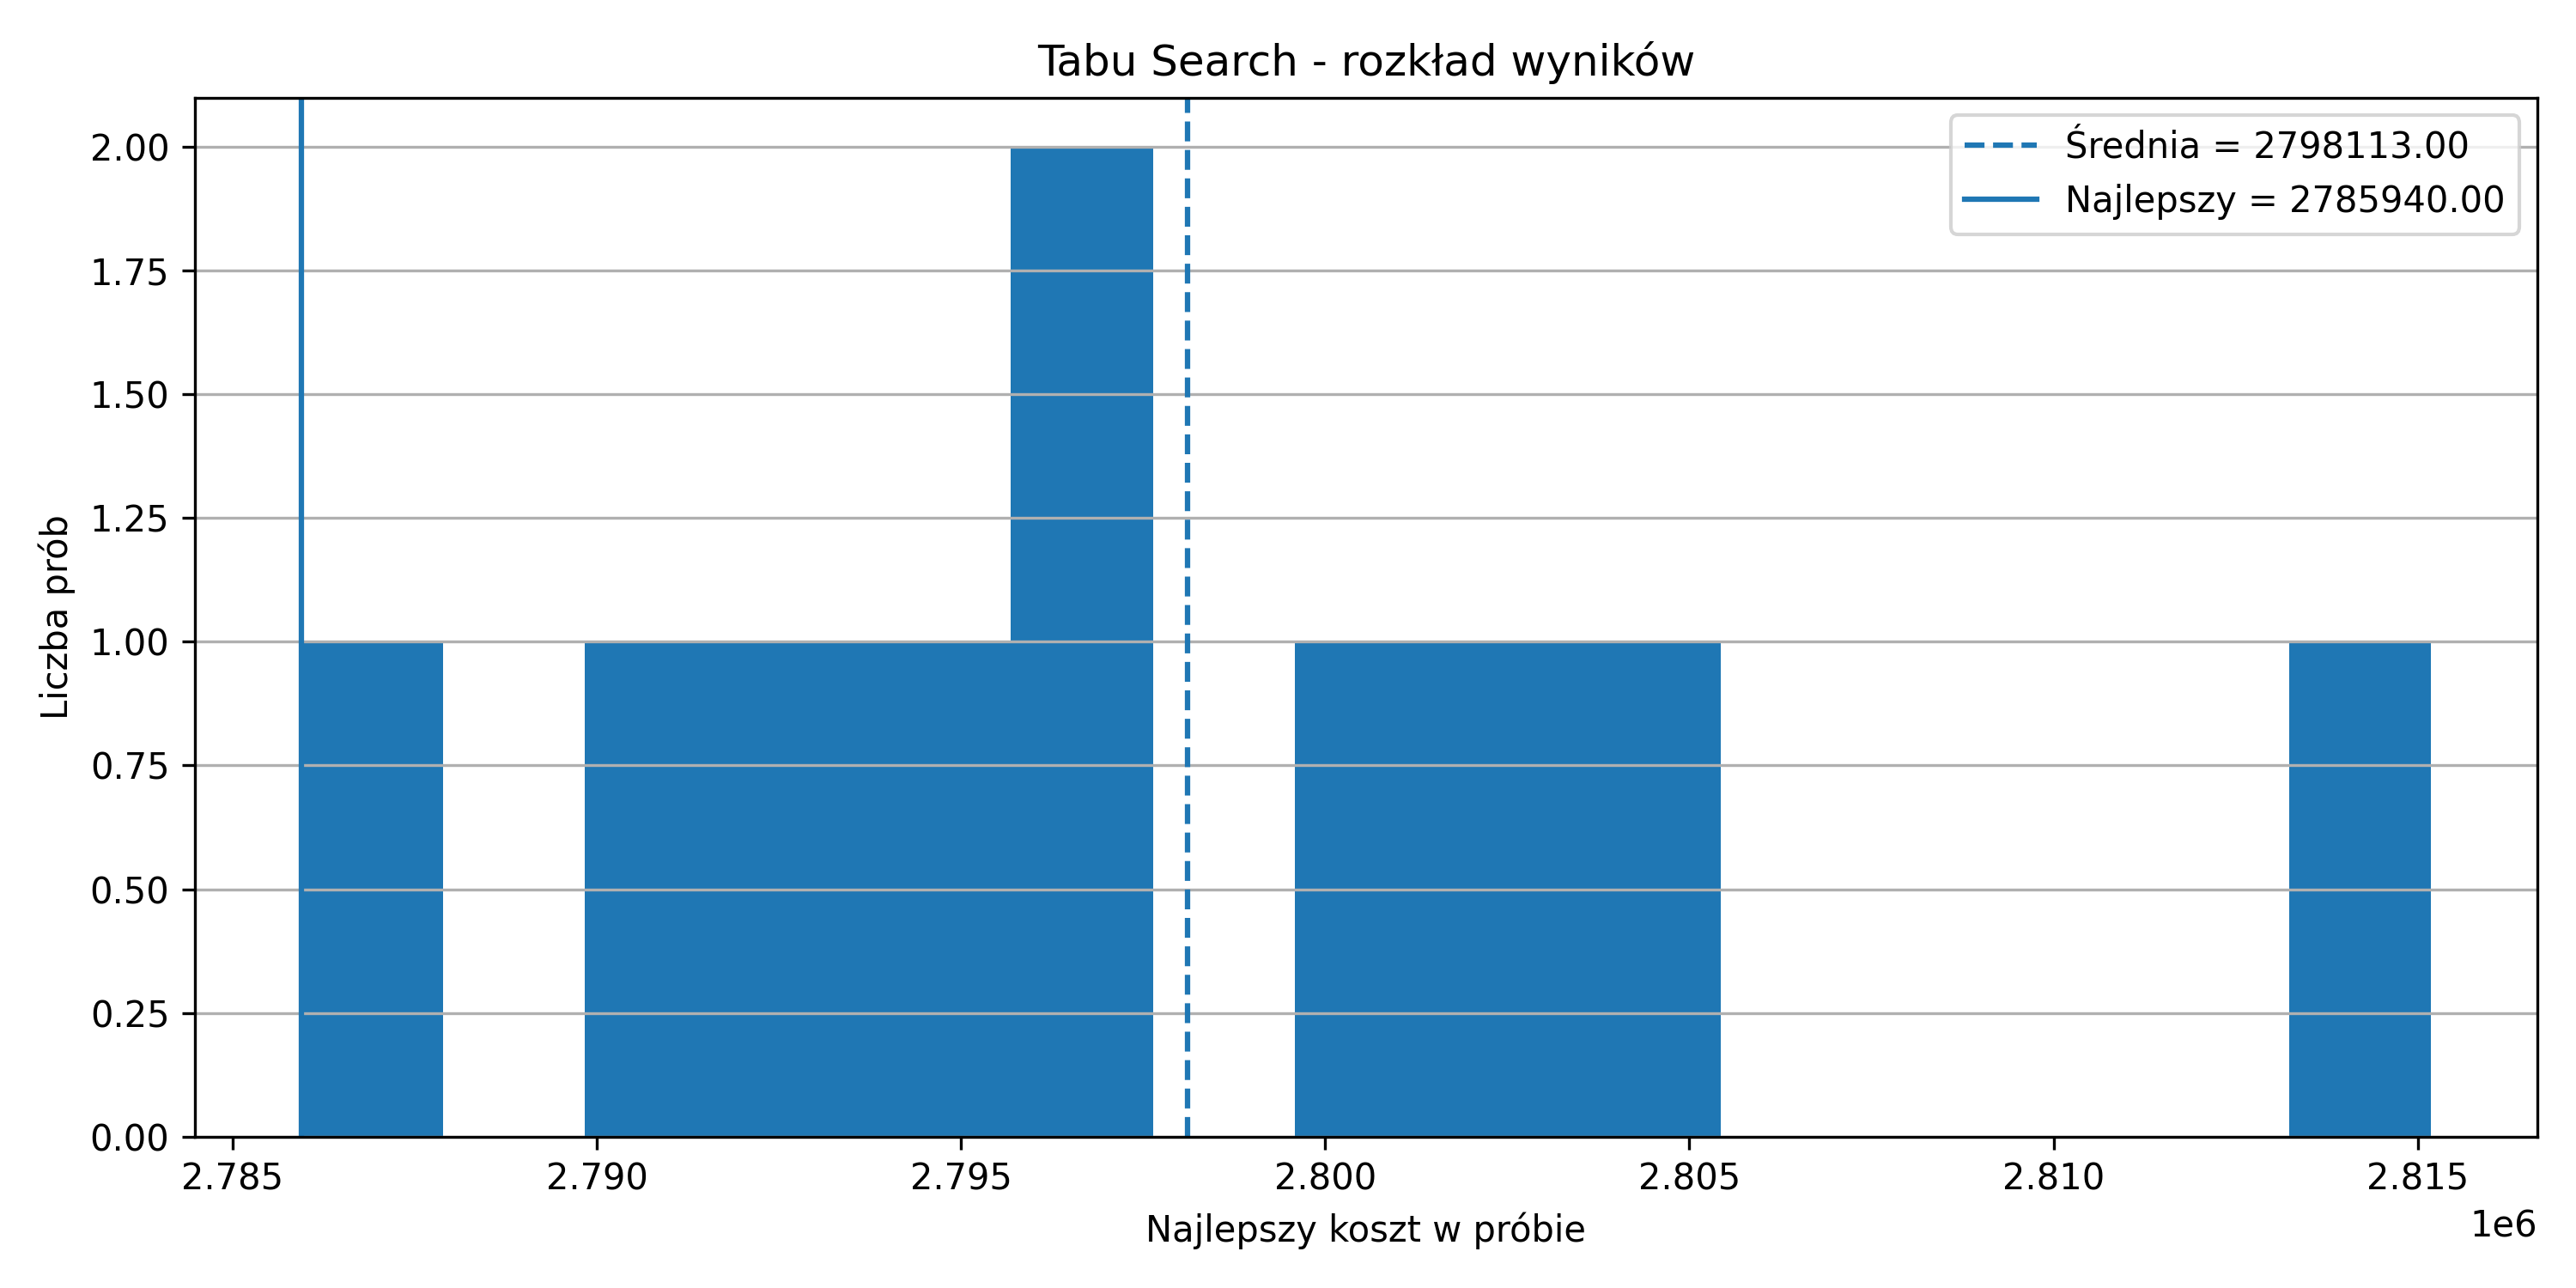
\includegraphics[width=0.9\textwidth]{tabu/tabu_runs_histogram_it16862.png}
    \caption{Rozkład wyników uzyskanych w próbach Tabu Search dla instancji \texttt{it16862.tsp}.}
\end{figure}

\begin{figure}[H]
    \centering
    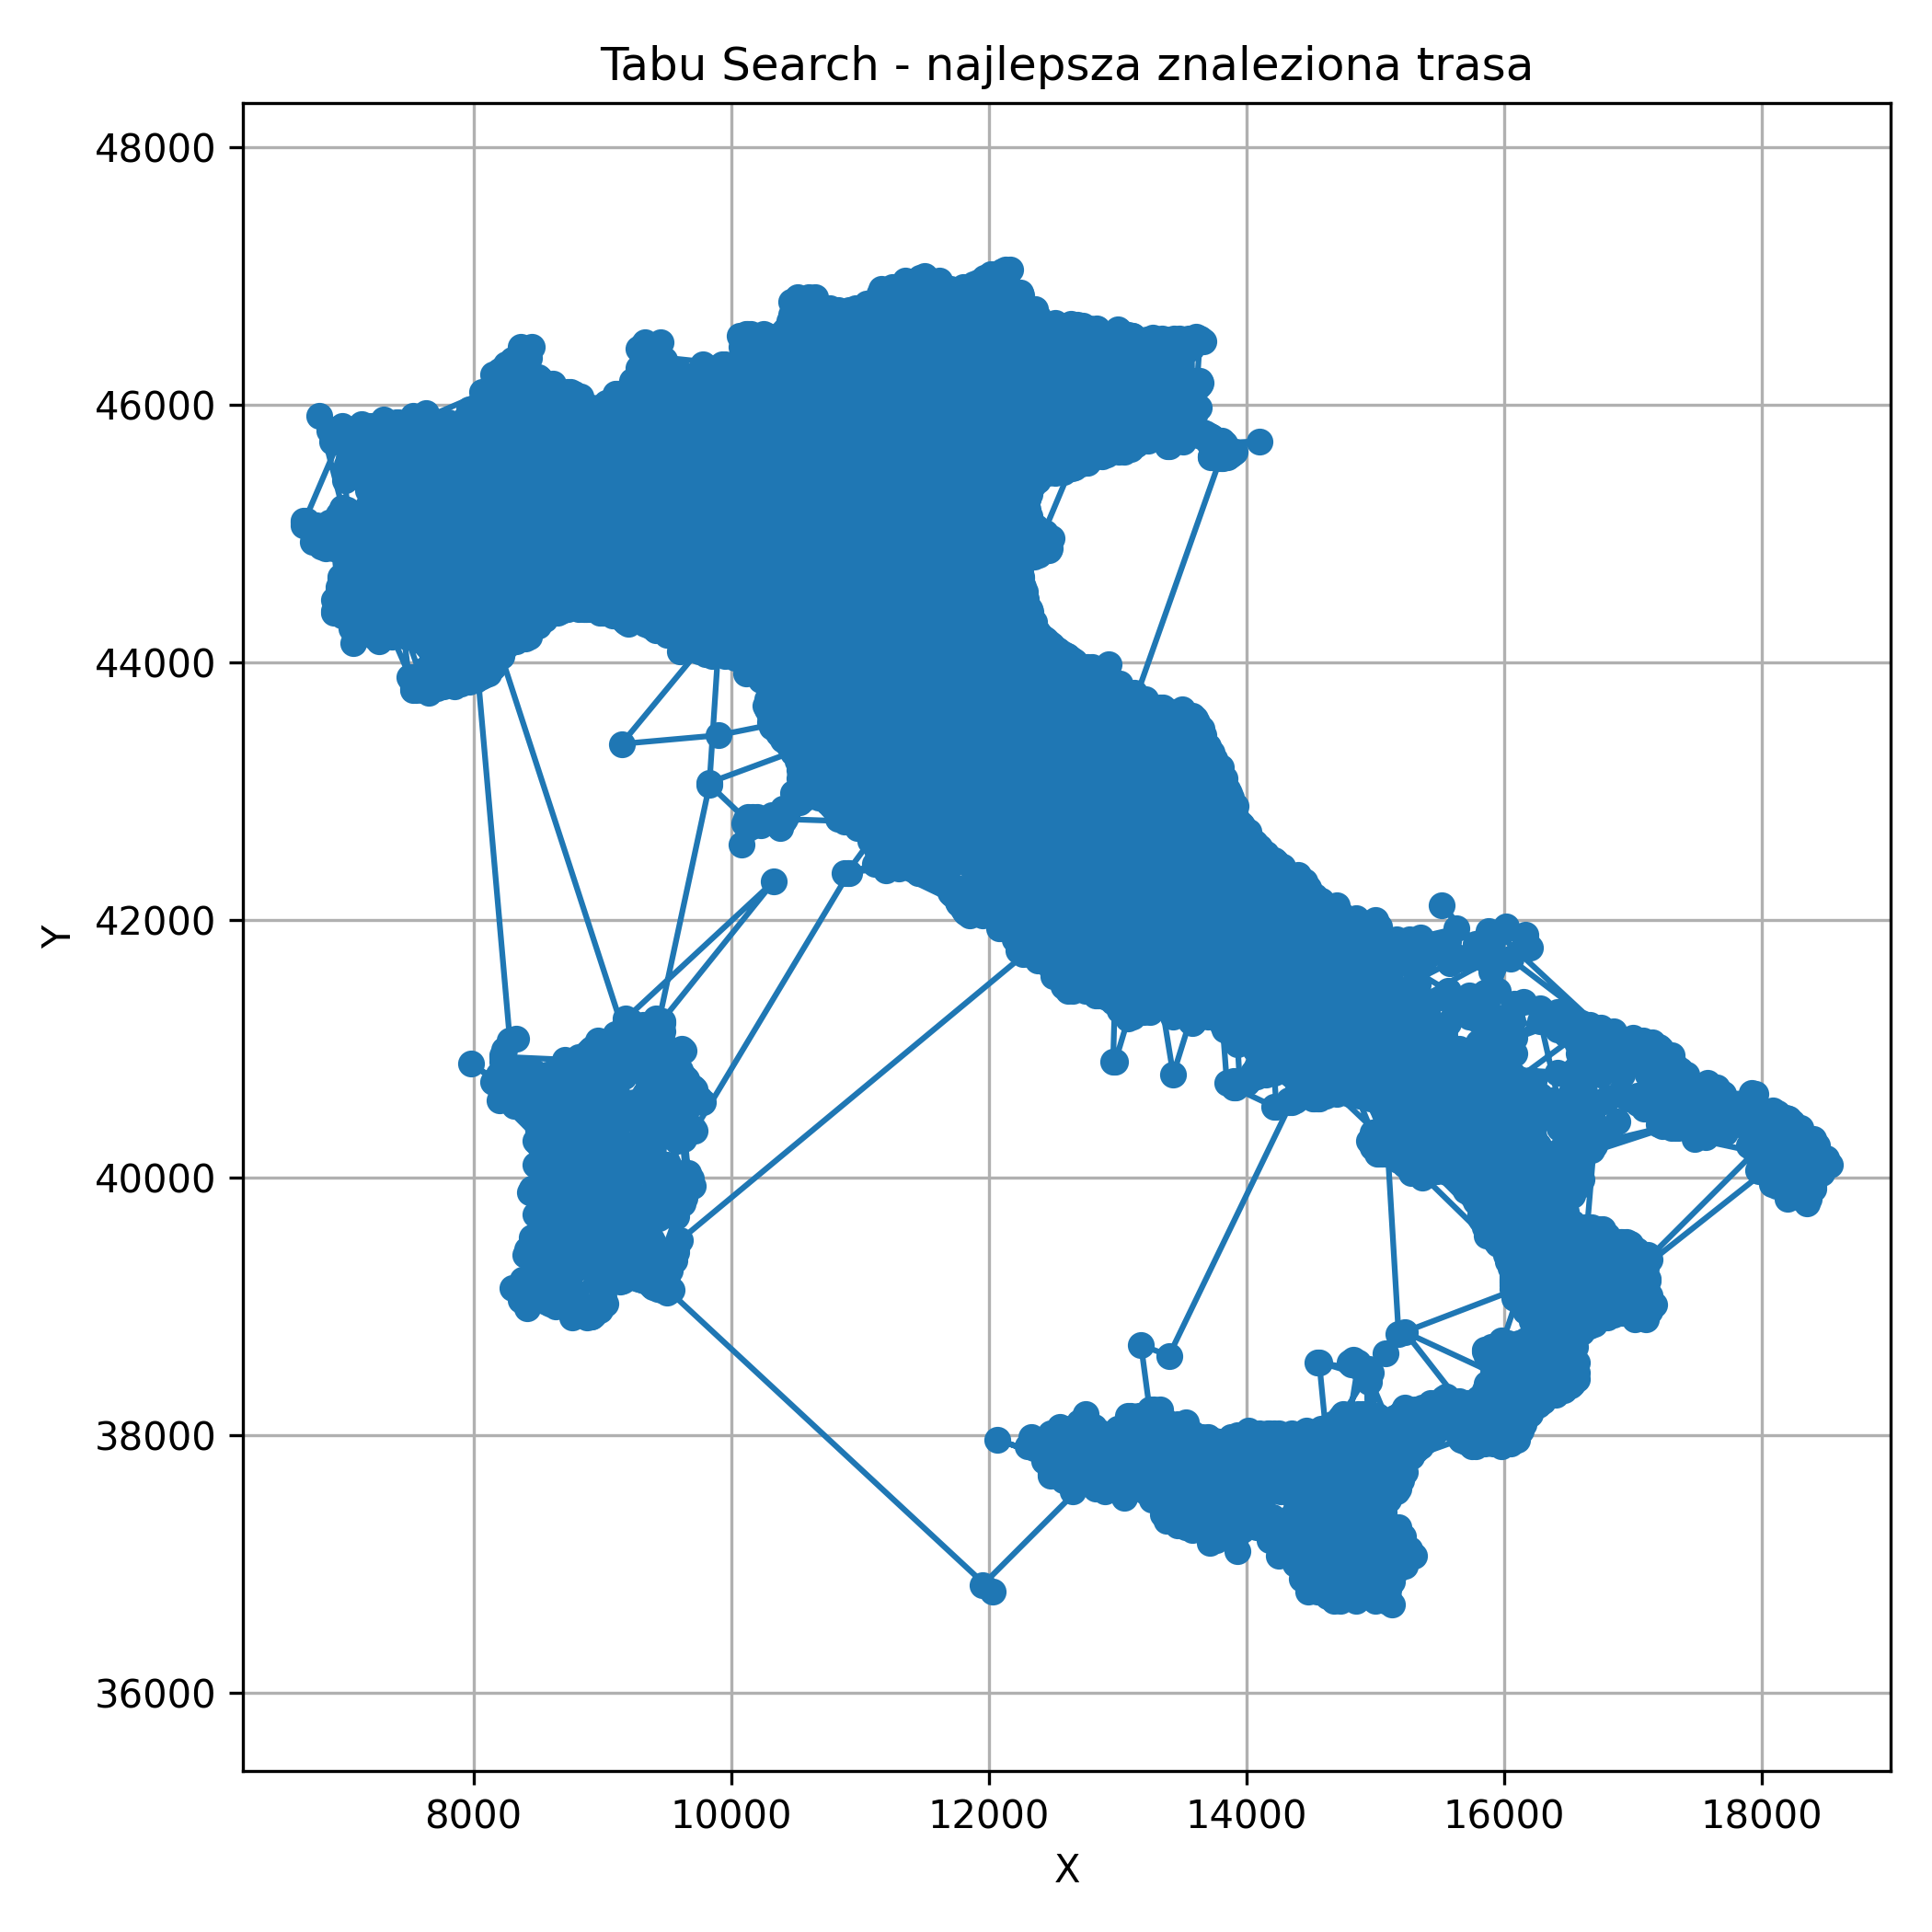
\includegraphics[width=0.8\textwidth]{tabu/tabu_best_route_it16862.png}
    \caption{Najlepsza trasa znaleziona przez Tabu Search dla instancji \texttt{it16862.tsp}.}
\end{figure}

\subsection{Wyniki Tabu Search}
\begin{table}[H]
    \centering
    \caption{Wyniki Tabu Search dla wykonanych prób.}
    \begin{tabular}{lrrrrr}
        \toprule
        Instancja & Najlepszy koszt & Średni koszt & Najgorszy koszt & Best Bound & \% \\
        \midrule
        \texttt{eg7146.tsp}  & 223422.0000  & 226059.1000  & 231414.0000  & 172387 & 129.60\% \\
        \texttt{ar9152.tsp}  & 1457410.0000 & 1468656.0000 & 1482070.0000 & 837479 & 174.02\% \\
        \texttt{it16862.tsp} & 2785940.0000 & 2798113.0000 & 2815180.0000 & 557315 & 500.00\% \\
        \bottomrule 
    \end{tabular}
\end{table}

\end{document}

